%% 
%% This is a sample doctoral dissertation.  It shows the appropriate
%% structure for your dissertation.  It should handle most of the
%% strange requirements imposed by the Grad school; like the different
%% handling of titles of one/many appendices.  It will automatically
%% handle the linespacing changes.  The body default is double-spaced
%% (except when you use the singlespace or condensed options).  The
%% default for quotations is single-space, and the default for tabularmultithreaded programs
%% environments is also single-space.  
%%
%% This class adds the following commands and environments to the
%% report class, upon which it is based:
%% Commands
%% ------------
%% \degree{name}{abbrv} -- Sets the name and abbreviation for the degree.
%%                         These default to ``Doctor of Philosopy''
%%                         and ``Ph.D.'', respectively.
%% \copyrightyear{year} -- for the copyright page.
%% \bachelors{degree}{institution} -- for the abstract
%% \masters{degree}{institution}   --  "
%%     if you have other degrees you may use
%% \secondbachelors{degree}{institution}
%% \thirdbachelors{degree}{institution}
%% \secondmasters{degree}{institution}
%% \thirdmasters{degree}{institution}
%% \priordoctorate{degree}{institution}
%%
%% \committeechair{name}           -- for the signature page
%% or, if you have two co-chairs:
%% \cochairs{first name}{second name}
%%
%% \firstreader{name}              --  "
%% \secondreader{name}             --  "
%% \thirdreader{name}              -- (optional)
%% \fourthreader{name}             --  "
%% \fifthreader{name}              --  "
%% \sixthreader{name}              --  "
%% \departmentchair{name}          -- for the signature page
%% \departmentname{name}           --  "
%%
%% \copyrightpage                  -- produces the copyright page
%% \signaturepage                  -- produces the signature page
%%
%% \frontmatter                    -- these are required in their various
%% \mainmatter                     -- appropriate locations
%% \backmatter                     --
%%
%% \unnumberedchapter[toc]{name}   -- like \chapter, except that it
%%                                    produces an unnumbered chapter;
%%                                    alternatively, like \chapter*,
%%                                    except that it lists the chapter
%%                                    in the table of contents.
%%
%% New environments:
%%   dedication  -- for the dedication
%%   abstract    -- for the abstract
%%
%% The thesis documentclass is built on top of the report document class.
%% It accepts all of the options that the report class accepts, plus the
%% following:
%%     doublespace -- the default, indicates double spacing as per U.Mass.
%%                    requirements.  You will need this when you do your
%%                    final copy.
%%     singlespace -- for earlier work, not acceptable to the Grad school
%%     condensed   -- for earlier work, not acceptable to the Grad school,
%%                    creates condensed versions of the frontmatter. 
%%                    Condensed implies singlespace.
%%     dissertation - the default, indicates that this document is a
%%                    dissertation.
%%     proposal    -- indicates that this document is a dissertation proposal,
%%                    rather than a dissertation.  This will only change the
%%                    wording on the title and signature pages.
%%     thesis      -- indicates that this document is a Master's thesis 
%%                    rather than a doctoral dissertation.  This also changes
%%                    the default for \degree to Master of Science, M.S.
%%     allowlisthypenation -- (the default), allows hyphenation of words in
%%                    the table of contents, the list of figures, and the list
%%                    of tables.  I believe that this is acceptable to the 
%%                    Graduate School.
%%     nolisthyphenation -- disallows hyphenation of words in the table of
%%                    contents and the list of figures and tables.  Use this 
%%                    option if the Grad School doesn't like your hyphenation.
%%     nicerdraft  -- relaxes some of the Grad School's rules for working with
%%                    drafts -- has no effect when doublespace is in effect
%%     nonicerdraft -- the default, leaves things in draft as they will be in
%%                     the final version
%% umthesis changes the default font size to 12pt, but you may specify 10pt or
%%   11pt in the options.
%%\documentclass[proposal]{umthesis}          % for Ph.D. dissertation or proposal
\documentclass{umthesis}          % for Ph.D. dissertation or proposal
%\documentclass{umthesis}          % for Ph.D. dissertation or proposal
% \documentclass[thesis]{umthesis}  % for Master's thesis

\usepackage{color}
\usepackage{listings}
\usepackage{amsmath}
\usepackage{amsfonts}
\usepackage{amssymb}
\usepackage{comment}
\usepackage{graphicx, subfigure}
\usepackage{url}
\PassOptionsToPackage{hyphens}{url}
\usepackage{pifont}% http://ctan.org/pkg/pifont
\usepackage{tabularx}
%\usepackage{hyperref}

%\lstset{ %
% language=C,                    % choose the language of the code
% basicstyle=\footnotesize,       % the size of the fonts that are used for the code
%numbers=left,                   % where to put the line-numbers
%numberstyle=\footnotesize,      % the size of the fonts that are used for the line-numbers
%stepnumber=1,                   % the step between two line-numbers. If it is 1 each line will be numbered
%numbersep=5pt,                  % how far the line-numbers are from the code
%backgroundcolor=\color{white},  % choose the background color. You must add \usepackage{color}
%showspaces=false,               % show spaces adding particular underscores
%showstringspaces=false,         % underline spaces within strings
%showtabs=false,                 % show tabs within strings adding particular underscores
%frame=single,           % adds a frame around the code
%tabsize=2,          % sets default tabsize to 2 spaces
%captionpos=b,           % sets the caption-position to bottom
%breaklines=true,        % sets automatic line breaking
%breakatwhitespace=false    % sets if automatic breaks should only happen at whitespace
%escapeinside={\%*}{*)}          % if you want to add a comment within your code
%}

%%
%% If you have enough figures or tables that you run out of space for their
%% numbers in the List of Tables or List of figures, you can use the following
%% command to adjust the space left for numbers.  The default is shown:
%%
%% \setlength{\tablenumberwidth}{2.3em}
\newcommand{\dthreads}{{\scshape Dthreads}}
\newcommand{\Dthreads}{{\scshape Dthreads}}
\newcommand{\Grace}{{\scshape Grace}}
\newcommand{\grace}{{\scshape Grace}}
\newcommand{\Sheriff}{{\scshape Sheriff}}
\newcommand{\sheriff}{{\scshape Sheriff}}
\newcommand{\SheriffProtect}{\textsc{Sheriff-Protect}}
\newcommand{\sheriffProtect}{\textsc{Sheriff-Protect}}
\newcommand{\sheriffprotect}{\textsc{Sheriff-Protect}}
\newcommand{\SheriffDetect}{\textsc{Sheriff-Detect}}
\newcommand{\sheriffDetect}{\textsc{Sheriff-Detect}}
\newcommand{\sheriffdetect}{\textsc{Sheriff-Detect}}
\newcommand{\Predator}{\textsc{Predator}}
\newcommand{\predator}{\textsc{Predator}}
\newcommand{\DoubleTake}{\textsc{DoubleTake}}
\newcommand{\doubletake}{\textsc{DoubleTake}}
\newcommand{\pthreads}{\texttt{pthreads}}
\newcommand{\cmark}{\ding{52}} %51 or 52
\newcommand{\xmark}{\ding{53}}% 53, 54, 55, 56
\newcommand{\CC}[1]{{\large \textbf{\color{red}CC:} \emph{#1} \newline}}
\lstdefinestyle{tt}{basicstyle=\small\ttfamily,keywordstyle=\bfseries,language=C, numbers=left, firstline=1}
%numberblanklines=false
\lstdefinestyle{rm}{basicstyle=\ttfamily,keywordstyle=\slshape,language=[LaTeX]{TeX}}


\begin{document}

%%
%% You must fill in all of these appropriately
\title{Reliable and Efficient Multithreading}
\author{Tongping Liu}
\date{May 2014} % The date you'll actually graduate -- must be
                     % February, May, or September
\copyrightyear{2014}
\bachelors{B.S.}{Harbin Institute of Technology}
\masters{M.E.}{Huazhong University of Science and Technology}
\secondmasters{M.S.}{UNIVERSITY OF MASSACHUSETTS AMHERST}
\committeechair{Emery D. Berger}
\firstreader{Scott F. H. Kaplan}
\secondreader{Yuriy Brun}
\thirdreader{Israel Koren}   % Optional
%\fifthreader{}            % Optional
%\sixthreader{}            % Optional
\departmentchair{Lori A. Clarke}
\departmentname{School of Computer Science}

%% If your degree is something other than a Ph.D. (for a dissertation), or
%% an M.S. (for a thesis), you will need to uncomment the appropriate
%% following line:
%%
%% \degree{Doctor of Education}{Ed.D.}
%% \degree{Doctor of Philosophy}{Ph.D.}
%%
%% \degree{Master of Arts}{M.A.}
%% \degree{Master of Arts in Teaching}{M.A.T.}
%% \degree{Master of Business Administration}{M.B.A.}
%% \degree{Master of Education}{M.Ed.}
%% \degree{Master of Fine Arts}{M.F.A.}
%% \degree{Master of Landscape Architecture}{M.L.A.}
%% \degree{Master of Music}{M.M.}
%% \degree{Master of Public Administration}{M.P.A.}
%%\degree{Master of Public Health}{M.P.H.}
%% \degree{Master of Regional Planning}{M.R.P.}
%% \degree{Master of Science}{M.S.}
%% \degree{Master of Science in Accounting}{M.S. Acctg.}
%% \degree{Master of Science in Chemical Engineering}{M.S. Ch.E.}
%% \degree{Master of Science in Civil Engineering}{M.S.C.E.}
%% \degree{Master of Science in Electrical and Computer Engineering}{M.S.E.C.E.}
%% \degree{Master of Science in Engineering Management}{M.S. Eng. Mgt.}
%% \degree{Master of Science in Environmental Engineering}{M.S. Env. E.}
%% \degree{Master of Science in Industrial Engineering and Operations Research}{M.S.I.E.O.R.}
%% \degree{Master of Science in Manufacturing Engineering}{M.S. Mfg. Eng.}
%% \degree{Master of Science in Mechanical Engineering}{M.S.M.E.}
%%
%% \degree{Professional Master of Business Administration}{P.M.B.A.}


%%
%% These lines produce the title, copyright, and signature pages.
%% They are Mandatory; except that you could leave out the copyright page
%% if you were preparing an M.S. thesis instead of a PhD dissertation.
\frontmatter
\maketitle
\copyrightpage     %% not required for an M.S. thesis
\signaturepage

%%
%% Dedication is optional -- but this is how you create it
%\begin{dedication}              % Dedication page
%  \begin{center}
%   \emph{ XXXXXX }       
%  \end{center}
%\end{dedication}

%%
%% Epigraph goes here...(aka frontispiece)
%% \chapter{Epigraph}?????

%%
%% Acknowledgements are optional...yeah, right.
\chapter{Acknowledgments}             % Acknowledgements page
%  Thanks to all those fine shepherds. Not to mention all the great
%  border collies and suchlike fine animals.

%%
%% Abstract is MANDATORY. -- Except for MS theses
I would first thank Emery Berger, my Ph.D. thesis advisor, for his wonderful supervision and enthusiastic support in the development of this thesis work. Emery taught me to work on those important and practical projects, and take everything seriously. I hope that I could be as lively, enthusiastic, and energetic as Emery one day to my students. I also thank my dissertation committee: Scott Kaplan, Yuriy Brun, and Israel Koren, for their valuable insights, feedback, and support. 

I am also fortunate to work with Chen Tian, Timothy Richards, Prashant Shenoy, Ziang Hu, Daniel Waddington, Seetharami Seelam, Wei Tan, Liana Fong, and Arun Iyengar. They provided me valuable guidance and suggestions on those projects we worked on together. I also thank Leeanne Leclerc, James Allan, and Laurie Downey for their help to make my experience at UMASS go as smoothly as possible. 

I couldn't finish my thesis without the help of PLASMA  labmates, including Charlie Curtsinger, Ting Yang, Gene Nowark, Kaituo Li, John Altidor, Divya Krishnan, Dan Barowy, Dimitar Gochev, John Vilk, Nitin Gupta, Jacob Evans, Justin Aquadro, and Emma Tosch. I also feel lucky to meet many friends in the computer science department, including Rui Wang, Ming Li, Tingxin Yan, Zongfang Lin, Kun Tu, Xiaojian Wu, Pengyu Zhang, Bo Jiang, Xiaozhen Tie, Fangyuan Zhou, Hong Zhang, Yue Wang, Wenzhao Liu, etc. I will never forget your help in my life. 

Finally, I would give my special thanks for my wife, Yuyu Tang. She quit her job to support my crazy idea of getting a Ph.D. degree. She also took care of most of the household duties and spent much of her time taking care of our two adorable kids, Yanbin Liu (Grace) and Yanlin Liu (Eileen). My buddy, Guangming Zeng, also deserves my special thanks for his generous help and valuable discussion when I chose the career in the computer science field. I also want to thank my kids, my late grandma, my parents, sisters, and brothers for their understanding and support.    



\begin{abstract}                % Abstract
The advent of multicore architecture has increased the demand for multithreaded programs. It is notoriously far more challenging to write parallel programs correctly and efficiently than sequential ones because of the wide range of concurrency errors and performance problems. 

In this thesis, I developed a series of runtime systems and tools to combat concurrency errors and performance problems of multithreaded programs.

The first system, \dthreads{}, automatically ensures determinism for unmodified C/C++ applications using the \pthreads{} library without requiring programmer intervention and hardware support. \dthreads{} greatly simplifies the understanding and debugging of multithreaded programs. \dthreads{} often matches or even exceeds the performance of standard thread libraries, making deterministic multithreading a practical alternative for the first time.

The second system attacks one notorious performance problem of multithreaded programs: false sharing. We provide the first accurate and precise detection tool,  \sheriffdetect{}, which can pinpoint the name of global variables or the allocation context of heap objects that involve in false sharing problems, without false positives.  However, rewriting a program to fix false sharing can be infeasible when source code is unavailable, or undesirable when padding objects can increase excessive memory consumption or further worsen runtime performance. To resolve this problem, we provide a runtime system, \SheriffProtect{}, to automatically boost the performance of programs with false sharing problems. 

The third system, \predator{}, improves the effectiveness of false sharing detection. It can detect one more type of false sharing: {\it read-write} false sharing. Also, it can even detect false sharing problems without occurrences, thus overcomes a shortcoming of all existing tools: they can only detect those observed false sharing problems. \Predator{} is the first tool to uncover false sharing problems of real applications. 

\end{abstract}

%%
%% Preface goes here...would be just like Acknowledgements -- optional
%% \chapter{Preface} 
%% ...


%%
%% Table of contents is mandatory, lists of tables and figures are 
%% mandatory if you have any tables or figures; must be in this order.
\tableofcontents                % Table of contents
%\listoftables                   % List of Tables
\listoffigures                  % List of Figures

%%
%% We don't handle List of Abbreviations
%% We don't handle Glossary

%%%%%%%%%%%%%%%%%%%%%%%%%%%%%%%%%%%%%%%%%%%%%%%%%%%%%%%%%%%%%%%%%%%%%%%%%
%% Time for the body of the dissertation
\mainmatter   %% <-- This line is mandatory

%%
%% If you want an introduction, which is not a numbered chapter, insert
%% the following two lines.  This is OPTIONAL:
\unnumberedchapter{Introduction}
For decades, applications enjoyed automatic and regular performance gains from increasing CPU speed.  However, the increase of CPU speed results in consuming more energy and generating more heat. Thus, Intel and other vendors have turned to providing multiple cores on a single machine. To take advantage of multiple cores, software needs to be written using multithreading. 

Building efficient and reliable multithreaded programs is still a challenging task because of the following reasons. First, concurrency requires programmers to think in an unnatural way that humans find difficult.  Second, existing languages and tools are inadequate to detect or prevent concurrency errors and performance anomalies. 

% Why we need determinism? Concurrency errors?
Concurrency errors of multithreaded programs, such as race conditions, atomicity violations, order violations, and deadlocks, are very hard to debug ~\cite{Lu:2008:LMC:1346281.1346323}, because their occurrences highly depend on some specific conditions, such as thread interleavings and CPU scheduling ~\cite{DBLP:conf/icse/BallBHMQ09,DBLP:conf/asplos/BurckhardtKMN10}. Instead of detecting possible concurrency errors, one promising alternative approach is to attack the problem of concurrency bugs by eliminating its source: non-determinism. A fully \emph{deterministic multithreading system} would prevent Heisenbugs by ensuring that executions of the same program with the same inputs always yield the same results, even in the face of race conditions in the code. Such a system would not only dramatically simplify debugging of concurrent
programs~\cite{Carver:1991:RTC:624586.625040} and reduce their attendant testing overhead, but would also enable a number of other applications. For example, a deterministic multithreaded system would greatly simplify record-and-replay for multithreaded programs~\cite{Choi:1998:DRJ:281035.281041,LeBlanc:1987:DPP:32387.32396} and the deterministic replication of a multithreaded application on different machines for fault tolerance~\cite{deterministic-process-groups,1134000,224058,replicant-hotos}.

% Why we need to find out false sharing problems.
It is also difficult to write efficient multithreaded programs. The {\it false sharing} problem is a notorious performance problem for multithreaded programs~\cite{falseshare:effect, falseshare:Analysis}. It occurs when multiple threads, running on different cores with their separate caches, access logically independent words in the same cache line. If a thread modifies  a cache line, the cache coherence protocol invalidates the duplicates of this cache line in other caches, which is crucial for true sharing cases. However, it is totally unnecessary for false sharing cases. False sharing can force one core to wait unnecessarily for updates from another processor, thus wasting both the CPU time and precious memory bandwidth. 

\subsection*{Contributions}

This thesis handles two categories of problems for multithreaded programs, {\it reliability} and {\it performance}. It makes the following contributions:

\begin{itemize}
\item \Sheriff{} framework: I developed a novel processes-as-threads framework derived from Grace~\cite{grace}. \sheriff{} is a software-only drop-in replacement of the stand \pthreads{} library. It turns threads into processes, with separate address spaces but a shared file table. \sheriff{} provides per-thread memory protection and isolation on page granularity by relying on the stand memory protection mechanism and a twinning-and-diffing mechanism. \sheriff{} enables a range of possible applications, including language support and enforcement of data sharing, software transactional memory, thread-level speculation, and race detection. 

\item I developed an efficient deterministic multithreading system, \dthreads{}, for unmodified C/C++ applications,  without programmer intervention and hardware support. \dthreads{} is based on the \sheriff{} framework to isolate executions of different threads. \dthreads{} outperforms the previous state-of-the-art runtime system (CoreDet) by a factor of 3, and often matches and sometimes exceeds the performance with the standard \pthreads{} library. \Dthreads{} enforces robust/stable determinism even in the face of data races, greatly simplifying program understanding and debugging: programs always behave identically, even with different inputs and on different hardware, as long as the synchronization order is the same. Because of this, \dthreads{} can also be used to support replicated executions of multithreaded applications for fault tolerance purposes.

\item 
Based on the \sheriff{} framework, I developed another two tools, \SheriffDetect{} and \SheriffProtect{}, to deal with false sharing problems of multithreaded programs, one of the notorious performance problems. 
\SheriffDetect{} find instances of false sharing accurately (no false positives), runs with low overhead (on average 20\%), and can pinpoint global variables and heap objects involving in false sharing. \SheriffProtect{} mitigates false sharing by adaptively isolating shared accesses on a cache line from different threads into separate physical addresses, effectively eliminating the performance impact of false sharing. It can automatically boost the performance of multithreaded applications with false sharing problems. 

\item I also developed a tool, \predator{}, to improve the effectiveness of false sharing detection. Instead of relying on the \sheriff{} framework to track memory writes, \predator{} employs compiler instrumentation to track read and write memory accesses, which make it possible to detect one more type of false sharing, {\it read-write} false sharing. \Predator{} also overcomes a key limitation of previous detection tools: existing tools can only detect observed false sharing problems. However, occurrences of false sharing highly depend on memory layout and size of a cache line, which are affected by a lot of dynamic properties. \Predator{} can predict potential false sharing that does not manifest in a given execution but may appear---and greatly degrade application performance—--in a slightly different execution environment. \Predator{} is the first false sharing tool able to automatically and precisely uncover false sharing problems in real applications, including MySQL and the Boost library.


\end{itemize}

\subsection*{Outline}
The rest of this thesis is organized as follows. Chapter~\ref{chapter:problems} describes reliability and performance problems of multithreaded programs, which we are going to handle in this thesis. Chapter~\ref{sec:sheriffframework} describes the processes-as-threads framework, \sheriff{}, which is the basis of \dthreads{}, \SheriffDetect{} and \SheriffProtect{}. Chapter~\ref{chapter:dthreads} describes \dthreads{} that ensures deterministic execution for multithreaded programs linking to this drop-in library. Chapter~\ref{chapter:sherifftools} discusses how to precisely detect and automatically tolerate false sharing problems based on the \sheriff{} framework. Chapter~\ref{chapter:preditor} describes a generalized false sharing detection tool by combining compiler instrumentation and runtime system, which improves the effectiveness of false sharing detection. 
Chapter~\ref{chapter:relatedwork} provides a substantial comparison between previous work and our approaches.  Chapter~\ref{chapter:conclusion} concludes the thesis with its contributions and possible future work. 


%%
%% Some sample text



\chapter{Problems of multithreaded programs}
\label{chapter:problems}

Writing Multithreaded programs can encounter concurrency errors and performance anomalies. This thesis discusses in detail two different types of problems, non-determinism and false sharing.  We discuss the definitions, causes of these problems and their possible consequence as follows.

\section{Non-determinism}
\label{sec:nondeterminism}

\subsection{Background}
Deterministic behavior of programs is the most desirable behavior: given the same input, a program
produces the same output and generates the same execution. Relying on this behavior, it is able to figure out problems of programs. 

In reality, it is relatively easy for sequential programs to achieve this target if a program do not explicitly rely on a randomized mechanism. 
However, it is hard to do this for parallel programs. In shared memory multithreaded programs, an application can only experience one of many possible 
schedules at a time. Thread scheduling, the order of memory accesses on the shared data, operations depending on timing and non-deterministic synchronizations, can easily lead to different executions of the same program.


\begin{figure*}[!ht]
{\centering
\fbox{
\subfigure{\lstinputlisting[numbers=none,frame=none,boxpos=t]{fig/nondeter.sample1}}
\hspace{20pt}
\subfigure{\lstinputlisting[numbers=none,frame=none,boxpos=t]{fig/nondeter.sample2}}
\hspace{20pt}
\subfigure{\lstinputlisting[numbers=none,frame=none,boxpos=t]{fig/nondeter.sample3}}
}
\caption{Non-determinism problem 
\label{fig:nondeterminism}}
}
\end{figure*}

A simple example of non-deterministic execution can be seen in Figure~\ref{fig:nondeterminism}. When using the standard \pthreads{} library, this program can print ``1,0'', ``0,1'' or ``1,1'' in the end, depending on the order of memory accesses from different threads. We actually run this simple program for one million times. About 99.43\% of time, it will print ``1,0'', while 0.56\% it will print ``0,1'' and 0.01\% it will print ``1,1''. According to the semantics of this program, both ``1,0'' and ``1,0'' are correct results. Thus, the unexpected result (``1,1'') caused by race conditions happens very rarely, only about 0.01\%.  
It is very difficult to observe/reproduce these rare cases that caused by race conditions.

\subsection{Source of Non-determinism}
Non-determinism can be caused by a lot of sources, both external sources and internal sources. For example, the timing of external inputs is one of the sources that can lead to non-determinism. This section only lists internal sources of non-determnism~\cite{costofdeterminism}. 
 
\emph{Thread Communication}: 
Thread communication is the most important source of non-determinism for multithreaded programs. 
First, the order of accesses on shared variables may change from one execution to the other. Second, the orders on shared resources, such as memory allocation, synchronization, and library/system calls, vary across different executions. 
Third, the interaction between compiler and run-time can be changed. For example, lazy binding may cause the thread that  performs address resolution to execute much more instructions than others. 

\emph{Memory Layout}: 
Address space layout randomization (ASLR) in Linux environment brings non-deterministic memory addresses of instructions and data across different executions. Thus, a program relying on memory addresses lead to non-deterministic execution of a program. 

\emph{System or Library Dependence}:
Some library or system calls cannot return deterministic results. For example, the \texttt{gettimeofday()} library call returns different time values at different time, and \texttt{read} system calls may return different number of bytes, depending on the timing of issuing \texttt{read} calls.  An application relying on them can execute non-deterministically too. 


\subsection{Effect of Non-determinism}
Because of different sources of non-determinism, listed in the above section, existing multithreaded applications can not run deterministically: given the same input, a program can have different executions that may or may not lead to different outputs. 

Non-determinism can greatly complicate the reasoning and debugging in development phases, which makes it hard for programmers to reproduce program errors. 
Even worse, since executions of deployment can vary from executions of development phase, a lot of programmer errors can be easily leaked to customers.

By contrast, determinism greatly simplifies the understanding and debugging of multithreaded programs. We can always guarantee the same executions on both development phases and the deployment phases, thus there is no need to worry about erroneous results. 

\section{False Sharing}
\label{sec:falsesharingproblems}

\subsection{Definition}
% What is the definition of false sharing?
False sharing occurs when different processors in a shared-memory parallel system are referencing distinct fields within the same coherence block (page or cache line) simultaneously, thereby inducing ``unnecessary'' coherence traffic~\cite{Bolosky:1993:FSE:1295480.1295483}. 

Although it is difficult or impossible to know where a thread runs in an actual execution, we can conservatively assume that different threads are running on different processors with separate cache. Thus, in the multithreaded environment, false sharing simply implies: multiple threads access distinct parts of the same cache line simultaneously, while one of them is a write operation. False sharing is shown in Figure~\ref{fig:fs}. 
Based on the relationship of false sharing objects, 
false sharing can be classified into inter-object and intra-object false sharing. When two different objects in the same cache line are accessed by different threads simultaneously, that is inter-object false sharing. Otherwise, it is intra-object false sharing. 

There is another concept, true sharing, which is opposite of false sharing. In true sharing (Figure~\ref{fig:ts}), multiple threads are accessing the same word. 

There is another way to differentiate false sharing with true sharing. False sharing is avoidable, while true sharing is not. 

\begin{figure*}
\begin{center} 
\subfigure[False sharing]{%
   \label{fig:fs}
   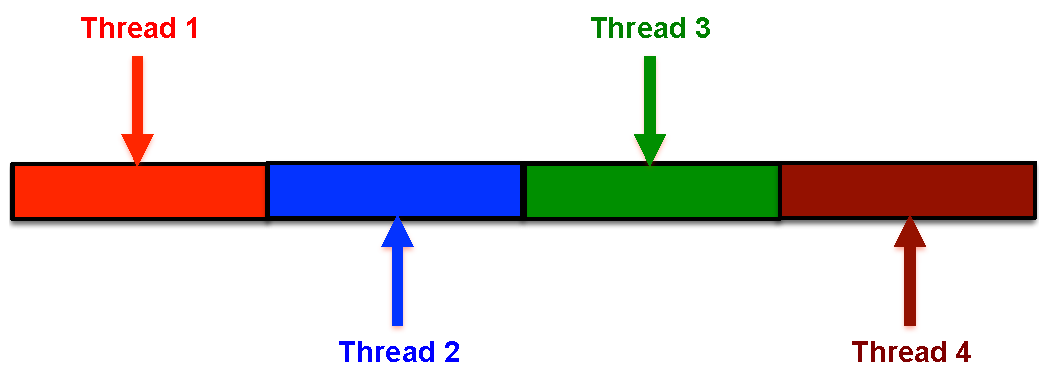
\includegraphics[width=2.4in]{sheriff/figure/falsesharing.pdf}
}%
\hspace{50pt}
\subfigure[True sharing]{%
   \label{fig:ts}
   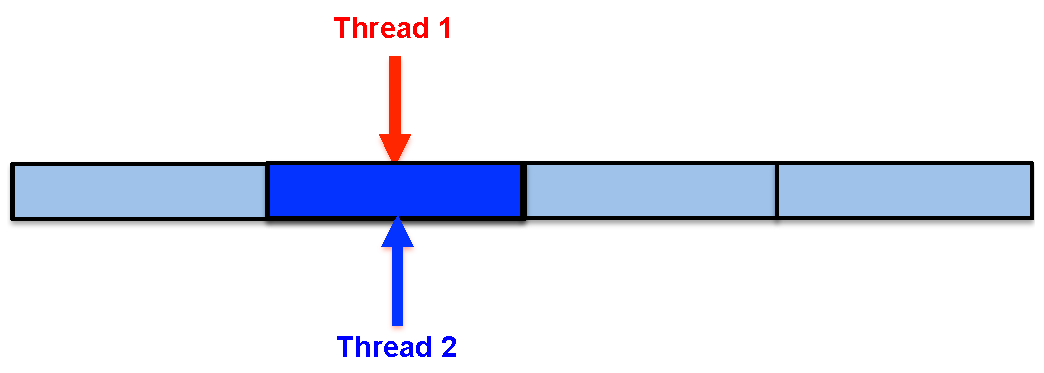
\includegraphics[width=2.4in]{sheriff/figure/truesharing.pdf}
}%
\end{center}
%\includegraphics{fig/potential.pdf}
\caption{False sharing and true sharing in a cache line with four words. }
\label{fig:fsexample}
\end{figure*}

% The classification of false sharing?

\subsection{Reason of False Sharing}

As shown in Figure~\ref{fig:fsexample}, false sharing only occurs when the size of coherence block is larger than that of a single word. Multiple processors may reference different words of the same coherence block. In this perspective, a single-word block size can avoid false sharing problems. 

However, using a single-word block size is not the actual case. In reality, the size of a coherence block (cache line) is normally 32 or 64 bytes. The reason of using multiple words in a cache line is to reduce the groups of transfers between the main memory and the cache since programs always have some spatial locality of reference. Those adjacent words are very likely to be referenced in the future.

From the performance perspective, reducing the coherence block size to one word may minimize the data to transferred, but can increase the number of transfers. Thus, the overhead of transferring less data at a time can be larger than the benefit of eliminating false sharing coherence traffic. Actually, the hardware trend of cache line is to increase the size of cache line, which makes false sharing problems increasingly common. 

\subsection{Performance Impact}
\label{falsesharing}
False sharing can greatly slowdown the execution of multithreaded programs, which depends on many factors, including the cache block size, data layout, program access patterns, and the cost of coherence operations~\cite{Bolosky:1993:FSE:1295480.1295483}. 

In a typical shared-memory system, each processor may have a separate cache. In order to increase the access speed, when a processor references a word, all the data inside the same cache line is fetched from the main memory to its corresponding cache. 
When multiple processors are accessing distinct words of the same cache line simultaneously, the shared data can be replicated into caches of different processors that access this cache line. Thus, it is very important to maintain the coherence across different processors: if any copy is changed, this change should be propagated to other processors immediately for correctness purposes. In real hardware, this data propagation only happens lazily when the data is accessed again, thus duplicates are invalidated at first. When a processor access an invalidated cache line, it should wait for the data propagating from other processors, wasting CPU time and memory bandwidth simultaneously. 

In the false sharing case, this propagation is totally unnecessary because different threads are actually accessing different parts of the same cache line. Thus, there is no need for a processor to get the updated data that is not going to access. However, hardware can only tracks the change of data on the granularity of a cache line and have to propagate those changes if any word has been changed. When there are interleaved writes, issued by different processors, on the same cache line, the ping-pong effect of loading-and-invalidating of data on this cache line can greatly slow the execution of programs. 
Programs with false sharing can even run slower in a multi-core machine than in a single-core machine, losing the benefit of multiple cores.  

Many common programming practices can easily cause false sharing. For example, different threads accessing different entries of the same global array, listed in Figure~\ref{fig:falsesharingexample}, is such an example. This example has no correctness problem, but a serious performance problem. 

\begin{figure*}[!ht]
{\centering
\fbox{
\subfigure{\lstinputlisting[numbers=none,frame=none,boxpos=t]{fig/falsesharing.sample1}}
\hspace{20pt}
\subfigure{\lstinputlisting[numbers=none,frame=none,boxpos=t]{fig/falsesharing.sample2}}
}
\caption{False sharing problem
\label{fig:falsesharingexample}}
}
\end{figure*}

We actually run this program on a real machine with 8 cores and Figure~\ref{fig:fsperfimpact} presents performance results. On this evaluation, we specifically choose a different number of threads, matching the number of hardware cores, from 1 thread to 8 threads, to perform the same amount of workload. We find out that false sharing can greatly impact the performance, which brings around $13\times$ difference between actual performance and the expected performance. Two trends--the prevalence of multicore architectures and
the expected increase in the number of multithreaded applications in broad use, and increasing cache line sizes--are likely to make false sharing increasingly common.

\begin{figure*}[!t]
\centering
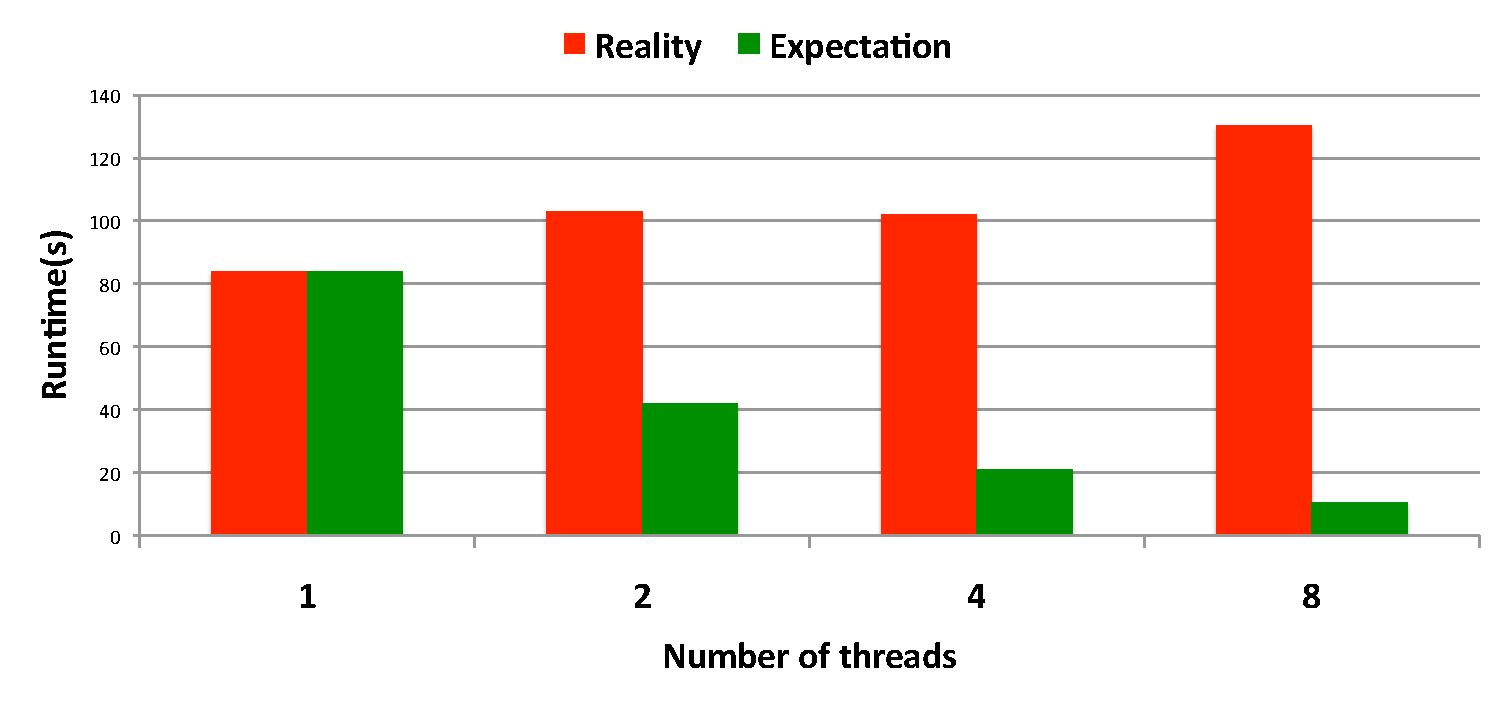
\includegraphics[width=6in]{fig/fsperfimpact.pdf}
\caption{
False sharing performance impact for the simple program shown in Figure~\ref{fig:falsesharingexample}.
\label{fig:fsperfimpact}
}
\end{figure*}

\subsection{Fixing False Sharing}
There are several ways to fix false sharing problems after they are identified. The basic idea is to prevent multiple threads from accessing the same cache line simultaneously.  

The first way is to change the size of corresponding structure or class, by padding some useless words. Thus, we can prevent two threads concurrently accessing the same cache line. One example of prevention, linear\_regression, can be seen in Section~\ref{sec:effecteval}.

The second way is to assign the value to thread-local variables at first. Then different threads only update their own local variables, and commit those changes back to the shared variable in the end. For example, the problem shown in Figure~\ref{fig:falsesharingexample} is fixed using this method, see Figure~\ref{fig:falsesharingexamplefix}. 

\begin{figure*}[!ht]
{\centering
\fbox{
\subfigure{\lstinputlisting[numbers=none,frame=none,boxpos=t]{fig/falsesharing.sample2fix}}
}
\caption{Fixing the false sharing problem shown in Figure~\ref{fig:falsesharingexample}.
\label{fig:falsesharingexamplefix}}
}
\end{figure*}

Some other approaches, to fix false sharing problems automatically, is described in detail in Section~\ref{sec:fspreventwork}, but they all suffer different shortcomings. 







%\chapter{\DoubleTake{}: Evidence-Based Dynamic Analysis}
%\input {doubletake/doubletakemain}

\chapter{Processes-As-Threads Framework}
\label{sec:sheriffframework}


%%%%%%%%%%%%%%%%%%%%%%%%%%%%%%%%%%%%%%%%%%%%%%%%%%%%%%%
% How to replace threads with processes ?
%  1. Replacing pthread_create() with fork
%  2. How to achieve the same semantics with multithreading? 
%     a. Thread Creation and Exits
%     b. Synchronizations?
%     c. Custom Memory Allocator. how to share memory across different threads
%     d. Twinning and diffing mechanism
%
%%%%%%%%%%%%%%%%%%%%%%%%%%%%%%%%%%%%%%%%%%%%%%%%%%%%%%%

\sheriff{} extends the processes-as-threads idea, first introduced in Grace~\cite{grace}, to be a drop-in replacement  of the standard \pthreads{} library. It interposes those thread-spawning calls and replaces them with \texttt{clone} system calls with \texttt{CLONE\_FILES} flag, turning threads into processes. Since different processes have separate address spaces and signal handlers, different processes can isolate their executions and employ page-based ``per-thread'' memory protection. In order to achieve the shared-memory semantics of multithreaded programs, \sheriff{} replaces synchronizations with process-based synchronizations (Section~\ref{sec:sheriffsync}), runs the regions between synchronizations in the isolation mode (Section~\ref{sec:sherifftransaction}), and commits process-private changes to the shared mapping (Section~\ref{sec:sharedmemory}). 

\begin{figure*}[!h]
\centering
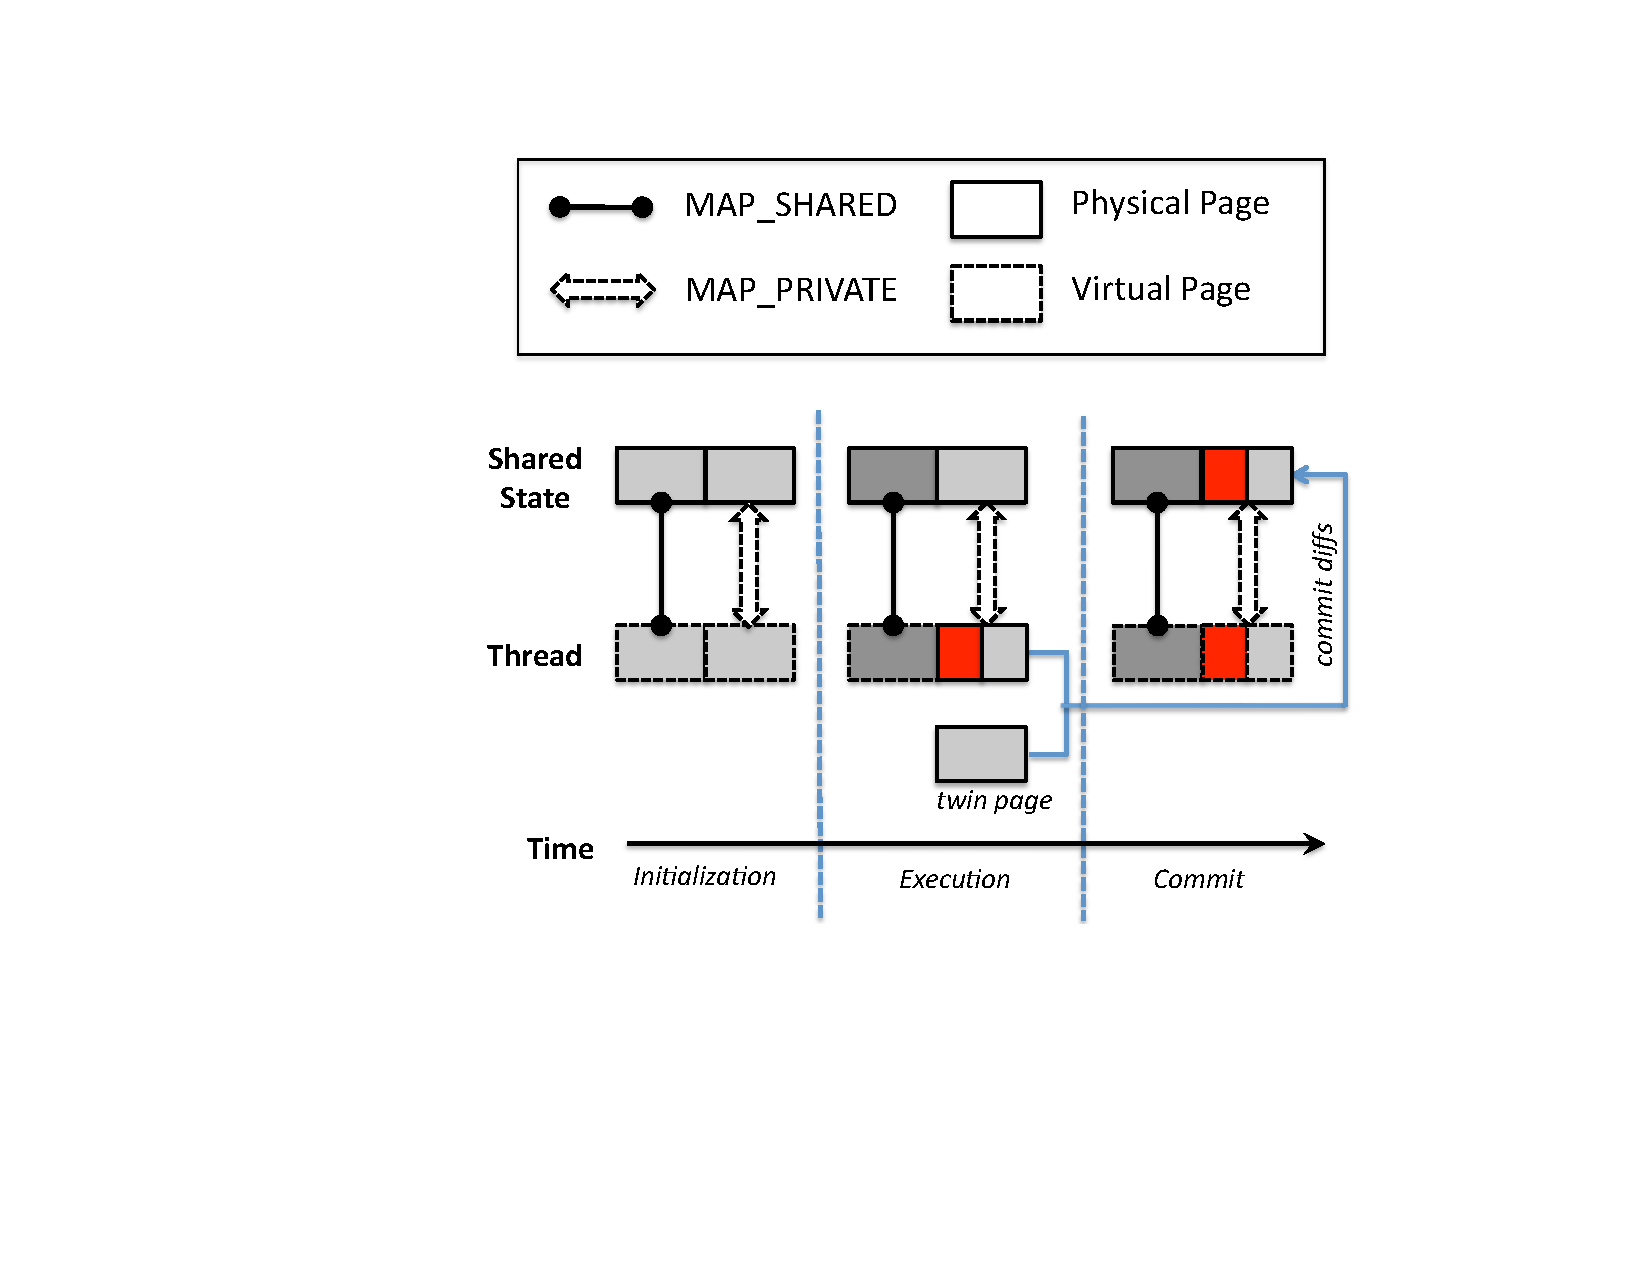
\includegraphics[width=6in]{sheriff/figure/sheriffframework.pdf}
\caption{
\Sheriff{} replaces threads with processes, thus it enables page-based ``per-thread'' memory protection and memory isolation. Upon synchronization points, local changes of different ``threads'' are committed to the shared state by comparing the difference between those working pages and their twin pages. \label{fig:overview}}
\end{figure*}

\section{Thread Creation and Exit}
\label{sec:threadcreat}

For thread creations, \sheriff{} interposes \texttt{pthread\_create()} functions and replaces them with \texttt{clone} system calls. 
By taking advantage of a feature of Linux that allows
selective sharing of memory and file descriptors, \sheriff{}
sets the \texttt{CLONE\_FILES} flag when creating new processes, resulting in child processes with different address spaces but the same shared file descriptor table. However, this attribute may not be applicable to other systems, e.g., Solaris. That would require shims on I/O operations to allow processes to share open file descriptors by sending
them over UNIX domain sockets~\cite[Section 17.4]{unixprogramming}.

For those children threads, \sheriff{} specifically invokes the \texttt{exit} function in order to exit those processes. For \texttt{pthread\_join}, joiners call \texttt{waitpid} to wait for a corresponding process to complete.  

\section{Synchronizations}
\label{sec:sheriffsync}

\sheriff{} supports the full range of synchronizations, including mutexes, conditional variables, barriers, and signals. 

By definition, synchronization is used to coordinate activities and data accesses among different threads. For example, a program calls \texttt{mutex\_lock()} before accessing the shared data. Leveraging on the processes-as-threads mechanism, \sheriff{} actually runs the regions between synchronizations in an isolated mode, which actually divides a program execution into different ``transactions.'' In the same transaction, all reads/writes happen only on private pages after the first write operation on those pages. Reads still perform on the shared mapping directly if a page is not written by the current thread.

At synchronization points, \sheriff{} commits those private changes of each thread to the shared mapping in order to achieve the shared memory semantics of multithreaded programs. Detailed implementation about the execution inside a transaction is discussed in Section~\ref{sec:sherifftransaction}. 

It is noted that the transaction concept here is different from that of transactional memory~\cite{transaction}. \sheriff{} does not support rollback and favors more on a longer transaction to better amortize the overhead. 

\sheriff{} turns threads into processes and runs an application in an isolated mode when there is no synchronization. But this isolation mechanism should not work for those synchronization variables. For example, in the mutex\_lock(), if a process only updates its private page holding this lock variable, then this update is not seen by other processes, which can cause multiple processes to enter into the same critical section concurrently. In order to coordinate different threads, \sheriff{} invokes process-based synchronizations on those synchronization variables that are shared across different processes, shown in Figure~\ref{fig:synccode}. Whenever there is a synchronization, \sheriff{} ends the current transaction, gets its process-shared variable, and synchronizes on this variable by using a process-based synchronization. To quickly locate its process-shared variable for a synchronization variable, \sheriff{} simply stores the pointer of it into the first word of this synchronization variable. 
 
\begin{figure}[!t]
\small
\begin{lstlisting}[style=tt]
void sync(var) {
  endTransaction();
  realVar = getRealVariable(var);
  sync_process_based(realVar);	
  beginTransaction();
}
\end{lstlisting}
\caption{Pseudo-code for a synchronization.\label{fig:synccode}}
\end{figure}

\section{Shared Memory Semantics}
\label{sec:sharedmemory}

In order to create the shared memory illusion for the process-as-threads framework, \sheriff{} employs the memory-mapped files to share the heap and globals across different processes, but not the stack. Different threads are using their own stacks and the stack is not used as a cross-thread communication in general.

\sheriff{} creates two different mappings for both the heap and the globals. One is a shared mapping, which is used to hold the shared state. Another is a private, copy-on-write(COW) mapping (per-process) that each process works on directly. User applications can only access  private mappings. 

Private mappings are linked to shared mappings through the same memory mapped file. In the isolated mode, reads initially go to the shared mapping until the first write on a page. After the first write operation, both reads and writes happen on the private mappings only. In order to achieve the shared memory illusion, \sheriff{} commits the current thread's local changes to the shared mapping at synchronization points using the twinning-and-diffing mechanism described in Section~\ref{sec:twinning-and-diffing}. More details of this are discussed in Section~\ref{sec:sherifftransaction}.

In the initialization phase, \sheriff{} checks its \texttt{/proc/pid/maps} file to find the range of its globals and creates a shared mapping for the globals. For the heap, \sheriff{} uses a customized memory allocator, which is discussed in Section~\ref{sec:customheap}. 

\subsection{Twinning-and-Diffing mechanism}
\label{sec:twinning-and-diffing}
In order to find out those local changes made by each thread, \sheriff{] borrows the twin page mechanism, which is introduced in TreadMarks and Munin~\cite{dsm:treadmarks, dsm:munin} for tracking modifications on a page in the distributed share memory system.

The basic idea is to create an additional ``twin'' page before the actual modification, by handling those memory protection faults. It is essential to ensure that the ``twin'' page is identical to its ``working'' page. To achieve this target, \sheriff{} issues a write operation to the original page, which specifically invokes a copy-on-write operation to create a ``working'' page. Then \sheriff{} creates a ``twin'' page by copying this ``working'' page. At synchronization points, \sheriff{} compares the ``twin'' page and its ``working'' page, using a byte-by-byte comparison, in order to find out those changes made by a thread: the difference of two pages simply implies the local changes made by the current thread. 

\subsection{Custom Memory Allocation}
\label{sec:customheap}

For the program heap, \sheriff{} replaces the default heap allocator with a BiBOP-style memory allocator, built on HeapLayers~\cite{heaplayers}. \sheriff{} pre-allocates a fixed chunk of memory from its underlying operating system using \texttt{mmap} system calls and satisfies memory allocations from this block by redirecting all memory allocations and deallocations. In the heap, all heap objects have the block size of {\it power of $2$}, using an object header to mark its status and size information. There is no split and merge operation on heap objects. If the size of an allocation is less than {\it power of 2}, \sheriff{} allocates an object with the size of the next {\it power of 2}.

In order to minimize possible false sharing induced by the memory allocator, \sheriff{} borrows a ``per-thread-heap'' idea from Hoard~\cite{Hoard}. \sheriff{} divides the heap into a fixed number of sub-heaps (currently 16), with the shared metadata of the super heap.  A thread can only allocate memory from its own sub-heap. When an object is freed, this object is returned to the subheap owned by the current thread. Since the subheap of each thread is allocated from different pages, this custom memory allocator is unlikely to allocate two objects from different threads on the same cache line, helping reduce the false sharing effect. 

\section{Execution of a Transaction}
\label{sec:sherifftransaction}

This section walks through an example of \sheriff{}'s execution from the beginning of a transaction to its termination. 

\emph{Transaction Begin:}
At the beginning of every transaction, \sheriff{} write-protects all shared pages so that later writes to these pages can be caught by handling SEGV protection faults.  

\emph{Inside a Transaction: }
Inside each transaction, \sheriff{} runs at the
same speed as a conventional multithreaded program for program reads. However, the first write to a protected page triggers a page fault that \sheriff{} handles: in the page fault handler, \sheriff{} obtains an exact copy of this page (a ``twin'' page), records the page holding the faulted address, and then unprotects this page so that future accesses run at full speed. Since \sheriff{} only exposes the private mapping to user applications, write accesses on a private mapping actually create a ``working'' page for every page written inside a transaction. 

Although protection faults are expensive,
these costs are amortized over the entire transaction because each page only incurs at most one page fault per transaction.
 
\emph{Transaction End:}
At the end of each transaction, at thread exits and before synchronization points, \sheriff{} commits local changes of a thread to the shared mapping to achieve the shared memory semantics. \sheriff{} commits only the differences between those ``twin'' pages and their ``working'' pages, using a byte-by-byte comparison. 

After those local changes are committed, \sheriff{} reclaims memory holding ``twin'' pages and ``working'' pages. \sheriff{} issues the \texttt{madvise} call, with the \texttt{MADV\_DONTNEED} flag, to discard those ``working'' pages.  Then, the current thread can observe those changes made by other threads from now on. 


\chapter{\dthreads{}:Efficient Deterministic Multithreading}

\label{chapter:dthreads}

As described in Section~\ref{sec:nondeterminism}, non-determinism can greatly complicate the reasoning and debugging of parallel programs. To resolve this problem, several recent software-only proposals aim at providing deterministic multithreading. However, all of these existing approaches suffer from a variety of disadvantages. Language-based approaches are effective at removing non-determinism but require programmers to write code in specialized languages, which can be impractical~\cite{Bocchino:2009:TES:1640089.1640097,Burckhardt:2010:CPR:1869459.1869515,Simpson:1999:SEE:330346.330357}. Recent deterministic systems that target legacy programming languages (especially C/C++) are either incomplete or impractical. Kendo ensures determinism of synchronization operations with low overhead, but does not guarantee determinism in the presence of data races~\cite{1508256}. Grace prevents all concurrency errors but is limited to fork-join programs, and although it is efficient, it requires code modifications to avoid large runtime overhead~\cite{grace}. CoreDet, a compiler and runtime system, enforces deterministic execution for arbitrary multithreaded C/C++ programs~\cite{Bergan:2010:CCR:1736020.1736029}. However, it exhibits prohibitively high overhead (running up to $8\times$ slower than \pthreads{}; see Section~\ref{sec:dthreadsevaluation}) and generates thread interleavings at arbitrary points in the code, complicating program reasoning, debugging, and testing.

\hspace{1em} \\
\noindent
\textbf{Contributions:}
We develop \textbf{\dthreads{}}, an efficient deterministic runtime system for multithreaded C/C++ applications. \dthreads{} guarantees deterministic execution of multithreaded programs even in the presence of data races (notwithstanding external sources of non-determinism like I/O): given the same sequence of inputs, a program using \dthreads{} always produces the same output. \dthreads{}'s deterministic commit protocol not only eliminates data races but also prevents lock-based deadlocks.

\dthreads{} is easy to deploy: it works as a direct replacement for the \pthreads{} library, requiring no code modifications or
recompilation. \dthreads{} is also very efficient. \dthreads{} leverages process isolation and virtual memory protection to track and isolate concurrent memory updates, based on the \sheriff{} framework. Not only does this approach greatly reduce overhead, comparing to approaches that track memory reads and writes, it also eliminates cache-line based false sharing, a notorious performance problem for multithreaded
programs. These two features combine to enable \dthreads{} to nearly match or even exceed the performance of \pthreads{} for the majority of benchmarks examined here. \dthreads{} thus marks a significant improvement over the state-of-the-art in deployability and performance, and provides promising evidence that fully deterministic multithreaded programming may be practical.

\section{\dthreads{} Overview}
Figure~\ref{fig:nondeterminism} shows an example multithreaded program that, because of data races, non-deterministically produces the outputs: ``1,0,'' ``0,1,'' and ``1,1.''  The order of instructions are changed from one execution to the other, resulting in these nondeterministic outputs. Using \dthreads{}, this program will \emph{deterministically} produce the same output ``1,1.'' Although this output can be a undesired one, the fact that results are always reproducible would make it easy for developers to reproduce and locate data races inside parallel programs.

\begin{figure}[h]
{\centering
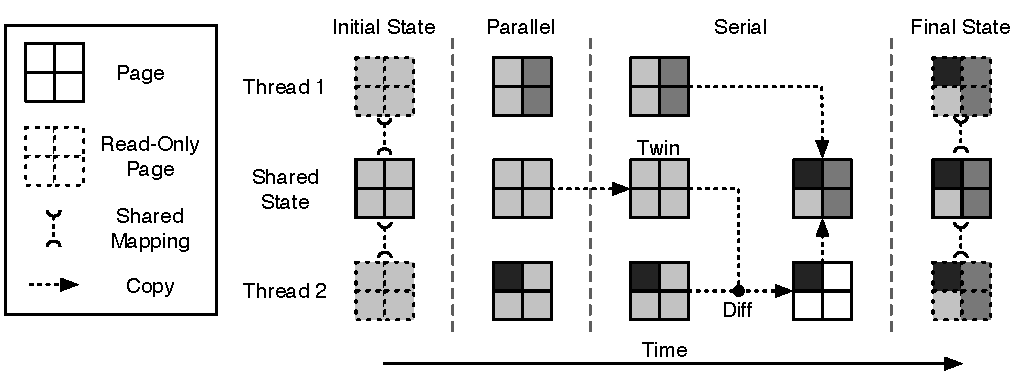
\includegraphics[width=6in]{dthreads/figure/architecture-diagram}
\caption{An overview of \dthreads{} execution.\label{fig:architecture}}
}
\end{figure}

\dthreads{} employs the following mechanisms to ensure the deterministic execution, illustrated by Figure~\ref{fig:architecture}: 

\textbf{Isolated Memory Access:} Based on the \sheriff{} framework, \dthreads{} runs threads as separate processes with private and shared views of memory, thus isolating executions of different ``threads.'' \dthreads{} uses this isolation mechanism to control the visibility of memory state, so that updates made by a thread cannot be seen by other threads if those updates are not committed explicitly to the shared mapping. By doing this, we guarantee that each ``thread'' can operate independently until synchronization points. Implementations are discussed in depth in Section~\ref{sec:threadsasprocs}.

\textbf{Deterministic Memory Commit:} 
Multithreaded programs use shared memory for communication, thus \dthreads{} must make a thread's changes seen by other threads. To guarantee determinism, \dthreads{} should publish updates of different threads in a deterministic order at deterministic points.

\dthreads{} actually commits the changes of a thread to the shared state in sequence at synchronization points. These points includes thread creation and exit; mutex lock and unlock; condition variable wait and signal; posix sigwait and signal; and barrier waits. Commits are ordered using a global token that is passed from one thread to the next; a thread can only commit when it holds the token.  The token-passing protocol is described in Section~\ref{sec:schedule} and the implementation of synchronization primitives is described in Section~\ref{sec:synchronization}.

\dthreads{} relies on the twinning-and-diffing mechanism to find out local changes of different threads, which has been discussed in Section~\ref{sec:twinning-and-diffing}. 

\textbf{Deterministic Synchronization:}
There is no deterministic guarantee on synchronizations under existing operating systems. Thus, \dthreads{} re-implements the full range of pthreads synchronization primitives and discusses  them in details in Section~\ref{sec:synchronization}. 

\hspace{1em} \\
\noindent
\textbf{Fixing the data race example} \\
About the example program in Figure~\ref{fig:nondeterminism},  \dthreads{} effectively isolates the execution from each thread until it completes, and then orders updates from different threads by thread creation time using a deterministic last-writer-wins protocol.

In the beginning of every execution, thread 1 and thread 2 have the same view of shared state, with a = 0 and b = 0. Since changes by one thread to the value of a or b are not visible to the other until this thread exits, both checks on two threads at line 2 will be true. So thread 1 sets the value of a to 1, and thread 2 sets the value of b to 1. These threads then commit their updates to the shared state and exit, with thread 1 always committing before thread 2. The main thread then should always print ``1, 1'' on every execution.

Determinism not only enables replay-without-recording and replicated executions, but also effectively converts ``Heisenbugs'' into ``Bohr'' bugs, making them reproducible. In addition, \dthreads{} optionally reports any conflicting updates due to racy writes, further simplifying debugging.


\section{\dthreads{} Architecture}

\begin{comment}
Because multithreaded programs frequently use updates to shared memory to communicate, \dthreads{} must implement a mechanism to expose one thread's updates to all other threads.  At the beginning of a transaction, all shared pages are protected, and can only be read by threads.  When a thread attempts to modify a shared page a local working copy is created, leaving the shared page unmodified.  At commit time, a ``twin'' copy of all modified pages is created.  Every page is compared to its twin (using a byte-wise diff) and modified bytes are copied back to the shared state.  Unlike transactional memory, conflicting changes do not result in rollbacks with \dthreads{}.  Further details are described in Section~\ref{sec:sharedmemory}.
\end{comment}


\label{sec:dthreads-architecture}
This section describes \dthreads{}’ key algorithms---isolated execution, deterministic (diff-based) memory commit, deterministic synchronization, and deterministic memory allocation---as well as other implementation details.

\begin{figure}
{\centering 
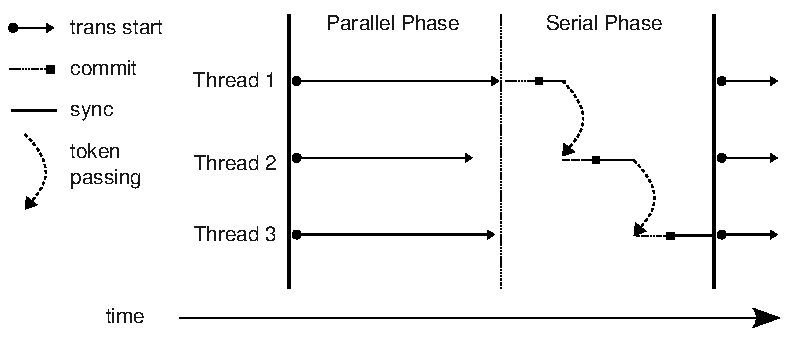
\includegraphics[width=6in]{dthreads/figure/phase}
\caption{An overview of \dthreads{} phase. Program execution with \dthreads{} alternates between parallel and serial phases.\label{fig:phase}}
}
\end{figure}

Figure~\ref{fig:phase} illustrates the execution of programs under \dthreads{}. \dthreads{} divides the execution of each thread into alternating parallel phases and serial phases. 
Based on the \sheriff{} framework, \dthreads{} isolates memory accesses in parallel phases. These accesses work on private copies of memory; that is, updates are not shared between threads during the parallel phases. When a synchronization point is reached, updates are applied (and made visible) in a deterministic order, as well as synchronizations. 
  
\subsection{Isolated Execution}
\label{sec:threadsasprocs}

Relying on the \sheriff{} framework, \dthreads{} turns threads into processes, with separate address spaces but the shared file table (Section~\ref{sec:threadcreat}). Thus, \dthreads{} isolates memory accesses among different threads between synchronization points: different threads can only see their own local changes. Those changes are merged together at synchronization points in order to achieve the shared memory semantics. 

\subsection{Deterministic Memory Commit}
\label{sec:sharedmem}

This section describes the mechanisms used to guarantee deterministic commits to the shared memory. These mechanisms are not provided by the \sheriff{} framework.   

\subsubsection{Fence and Token}
\label{sec:schedule}

\dthreads{} places internal fences between parallel and serial phases. \dthreads{} re-implements the fence because the standard \pthreads{}'s barrier mechanism does not support dynamic changes of threads number. 

\begin{figure}
\begin{lstlisting} [style=tt]
void waitFence(void) {
  lock();
	
  while(!isArrivalPhase()) { 
    CondWait();
  }

  waiting_threads++;
  if(waiting_threads < alive_threads) {
    while(!isDeparturePhase()) {
      CondWait();
    }
  } 
  else {
    setDeparturePhase();
    CondBroadcast();
  }

  waiting_threads--;
  if (waiting_threads == 0) {
    setArrivalPhase();
    CondBroadcast();
  }

  unlock();
}

\end{lstlisting}
\caption{Pseudocode for the internal fence.\label{fig:internalFence}}
\end{figure}

Figure~\ref{fig:internalFence} shows the pseudocode code for the internal fence. Threads must wait at an internal conditional variable until all threads depart from the last departure phase (lines 4-5). Then those threads are waiting at the fence until all alive threads have arrived at the same fence (lines 8-11). The last thread initiates the departure phase and wakes up all threads on the conditional variable (lines 14-15). As threads leave the fence, they decrement the number of waiting threads.  The last thread to leave sets the fence to the arrival phase and wakes any waiting threads (lines 19-21).

To reduce overhead, whenever the number of running threads is less than or equal to the number of cores, waiting threads use spin locks, instead of expensive cross-process \pthreads{} mutexes. When the number of threads exceeds the number of cores, \dthreads{} falls back to using \pthreads{} mutexes.

\begin{figure}
\begin{lstlisting} [style=tt]
void waitToken() {
  waitFence();
  while(isNotMyToken()) { yield(); }
}
void putToken() {
  passTokenToNextOfTokenQueue();
}
\end{lstlisting}
\caption{Pseudocode for waitToken and putToken. 
\label{fig:token}}
\end{figure}

Another key mechanism of \dthreads{} is the global token, which \dthreads{} uses to order memory commits and synchronizations. The token implementation is listed in Figure~\ref{fig:token}. The token is a shared pointer that points to the next runnable thread entry, which guarantees the global order for all operations in serial phases.  

\dthreads{} introduces two subroutines to manage tokens.  The \texttt{waitToken()} function first waits at the internal fence and then waits to acquire the global token in order to enter or leave the serial phases. The \texttt{putToken()} function passes the token to the next thread in the token-passing queue. 

As shown in Figure~\ref{fig:phase}, it is very important for a thread to wait at the internal fence before a thread enters or leaves serial phases, even for a thread that is guaranteed to have the token next. Otherwise, memory commits of a thread can affect other threads' behavior, bringing non-deterministic behavior for programs. 

\subsubsection{Commit Protocol}

Figure~\ref{fig:architecture} shows the steps to track modifications of every thread and expose them in a deterministic order.  

At the beginning of parallel phases, different threads have a read-only mapping for all shared pages. In parallel phases, if a thread writes to a page, this write is trapped in order to create a private copy and a identical twin page for this page. After that, reads and writes on this page happen on the private copy only. For those non-trapped pages, reads still go directly to the shared state.  

In serial phases, threads first commit their local changes that made in last parallel phase, guided by the global token.  The first thread  committing to a page can directly copy its private working copy to the shared state (page-based commits), but subsequent commits can only commit the modified bytes (byte-based commits), using the twinning-and-diffing mechanism discussed in Section~\ref{sec:twinning-and-diffing}. The byte-based commits are much slower than the page-based commits, but  they won't overwritten changes committed by those predecessors.  After a thread commits its local changes, it issues synchronizations before it passes the token to its next thread in the token-passing queue. 

In the end of serial phases, every thread has to release those private pages and twin pages, recover the read-only mapping, wait at the internal fence before entering into the next parallel phase. By removing those private pages and recovering those mappings, a thread is able to observe changes made by other threads, achieving the shared memory semantics. 

\subsection{Deterministic Synchronization}
\label{sec:synchronization}

\dthreads{} supports the full range of synchronizations of \pthreads{} library, including locks, conditional variables, barriers and different types of thread exits. Since the \sheriff{} framework can not provide any deterministic guarantee, \dthreads{} implements different types of synchronizations in a deterministic way as follows. 

\subsubsection{Locks}
Before a thread acquires a lock, it has to wait for the global token, by calling \texttt{waitToken}. 

\dthreads{} treats multiple locks as the same one. It only ends the current serial phase for a thread when all locks held by this thread are released. Because of that, it is possible for a program to avoid deadlock problems. 

At acquisitions of locks, \dthreads{} checks at first whether the current thread is already holding any locks. If not, the thread first waits for the token, commits those changes happened in the last parallel phase to the shared state, and begins a new atomic section. Then it increments the number of locks that it is currently holding before entering into critical sections. 

At deacquisitions of locks, \dthreads{} decrements the number of locks that the current thread holds first. A thread does nothing if it still holds some locks, with the number of locks not equal to 0. If all locks are released, \dthreads{} commits the memory changes made in this serial phase to the shared state. Then it passes the global token to the next thread in the token-passing queue, and waits on the internal fence before entering into the next round's parallel phase.

\subsubsection{Condition Variables}
\label{sec:condwait}

Guaranteeing determinism for condition variables is much more complex than for other synchronization primitives. The underlying operating system can not guarantee that threads are going to be waken-up in the same order as their waits. Thus, a naive implementation easily leads to a no-progress problem if the first waken-up thread can not get the global token to proceed first.

When a thread calls \texttt{pthread\_cond\_wait}, it first acquires the global token and commits local modifications made in the current serial phase since \texttt{pthread\_cond\_wait} is generally issued inside a critical section. It then removes itself from the token-passing queue, so that those threads waiting on condition variables do not participate in the token pass. Then, it adds itself to the conditional variable's waiting queue, decreases the number of alive threads (used in the internal fence mechanism), and passes the token to the next thread in the token-passing queue before actually waiting on a process-shared conditional variable. 

When a thread is awaken, it should check at first whether the current thread is ready to run or not. For a deterministic reason, \texttt{pthread\_cond\_signal} should only wake up the first thread waiting on a conditional variable and \texttt{pthread\_cond\_broadcast} wakes up all waiting threads. However, the underlying operating system, like Linux, can not guarantee this. To resolve this problem, in \texttt{pthread\_cond\_signal}, we specifically wake up all threads, but only the first thread is given the permission to run: If a thread is not able to run, it waits on this conditional variable again; If a thread is the candidate thread to be waken up, it waits for the global token to enter into the next serial phase; The candidate thread should get the token immediately in order to avoid a no-progress problem. 

For both \texttt{pthread\_cond\_signal} and \texttt{pthread\_cond\_broadcast}, the calling thread first waits for the global token, and then commits any local modifications before issuing an actual wake-up signal. When no threads are waiting on a condition variable, it passes the token to the next thread immediately, treating those calls as no-ops basically. Otherwise, it migrates corresponding threads, one for \texttt{pthread\_cond\_signal} and all for \texttt{pthread\_cond\_broadcast}, from the queue of this condition variable to the head of the token-passing queue, marks them as ready, increments the number of alive threads, and passes the token to the first thread in the token queue. 

\subsubsection{Barriers}

\label{sec:barrierwait}

Threads waiting on a barrier should not disrupt the token passing of running threads: \dthreads{} removes those waiting threads from the token-passing queue, and places them in corresponding barrier queue.

In order to ensure determinism, the calling thread first waits for the global token to commit any local modifications. If the current thread is the last one to enter the barrier, it moves all threads on the barrier queue to the token-passing queue, increases the number of alive threads, and passes the token to the first thread in the barrier queue. Otherwise, it removes itself from the token-passing queue, places itself in the barrier queue, releases the token, and waits on this actual barrier.


\subsubsection{Thread Creation and Exit}

\label{sec:threadcreation}

\begin{figure}
\begin{lstlisting} [style=tt]
void thread_create () {
  waitToken();
  clone(CLONE_FS| CLONE_FILES | CLONE_CHILD);
  if(isChild) {
    allocGlobalThreadIndex();
    insertToTokenQueue();
    notifyChildRegistered();
	// Wait for the parent to reach next sync point
    waitParentBroadcast();	
  }
  else if (isParent) {
    waitChildRegistered();
  }
}
\end{lstlisting}
\begin{lstlisting} [style=tt]
void thread_exit() {
  waitToken();
  atomicEnd(false);
  removeFromTokenQueue();
  decreaseInternalFence();
  putToken();
  exitThread(); 
}
\end{lstlisting}
\caption{Pseudocode for thread creation and exit($\S$~\ref{sec:threadcreation}).
\label{fig:threadcreation}
}
\end{figure}

To guarantee determinism, thread creations and exits must be performed in serial phases. 

In order to improve the parallelism and performance, a thread is allowed to create multiple threads without waiting for a new serial phase. Figure~\ref{fig:threadcreation} shows the pseudocode for thread creation and thread exit. First, the calling thread waits for the global token before proceeding (line 2). It then creates a new process, with shared file descriptors but a distinct address space, by invoking the \texttt{clone} system call (line 3).  Then the parent thread is waiting until its newly spawned child has registered itself. 

The newly spawned child obtains the global thread index (line 5), places itself in the token-passing queue (line 6), and notifies the parent that registration has finished(line 7). Then it waits for the notification from the parent to proceed when the parent to reach the next synchronization point, not a thread creation.  In this way, we can allow a parent thread to create multiple children threads in the same serial phase. 

When \texttt{thread\_exit()} is called, the caller first waits for the global token before committing any local modifications (line 3). It then removes itself from the token-passing queue (line 4), and decreases the number of alive threads (line 5). Finally, it passes the global token to the next thread in the token queue (line 6) and exits (line 7).

\subsubsection{Thread Cancellation}

\dthreads{} performs thread cancellations in serial phases for the deterministic reason. A thread can only invoke \texttt{pthread\_cancel} while holding the global token. If the thread being cancelled is waiting on a condition variable or a barrier, it is removed from the queue deterministically. Finally, to cancel a thread, \dthreads{} kills the target process using kill(tid, SIGKILL) and decrements the number of alive threads after the cancellation.

\subsection{Deterministic Memory Allocation}
Sometimes, programs may rely on the addresses of objects returned by the memory allocator intentionally (for example, by hashing objects based on their addresses), or accidentally. A program with a memory error, like a buffer overflow, will yield different results for different memory layouts.

The reliance on memory addresses can undermine other efforts to provide determinism. For example, CoreDet is unable to fully enforce determinism because it relies on the Hoard scalable memory allocator~\cite{Bergan:2010:CCR:1736020.1736029}. Hoard was not designed to provide determinism and several of its mechanisms, thread id based hashing and non-deterministic assignment of memory to threads, lead to nondeterministic execution in CoreDet for the Canneal benchmark. To resolve this problem, \dthreads{} employs both deterministic thread index and custom memory allocation mechanism. 

\subsubsection{Deterministic Thread Index}
\label{sec:threadindex}

POSIX does not guarantee deterministic process or thread identifiers. To avoid exposing this nondeterminism to threads that run as processes, \dthreads{} shims \texttt{pthread\_self()} in order to return a deterministic thread index on different executions. This thread index is managed using a single global variable that is incremented on every thread creation.  This unique thread index is also used to manage per-thread heaps and as an index into an array of thread entries.

\subsubsection{Custom Memory Allocation}

To preserve determinism in the face of intentional or inadvertent reliance on memory addresses, we designed the \dthreads{} memory allocator to be fully deterministic. 

\dthreads{} assigns subheaps to each thread based on its deterministically assigned thread index. In addition to guarantee the same mapping of threads to subheaps on different executions, \dthreads{} allocates superblocks (large chunks of memory) deterministically by acquiring a lock (under the global token) on each superblock allocation. Thus, threads always use the same subheaps, and these subheaps always acquires the same superblocks on each execution. The superblocks themselves are allocated via mmap: while \dthreads{} could use a fixed address mapping for the heap, we currently simply disable ASLR to provide deterministic mapping from mmap calls. If a program does not rely on absolute addresses, \dthreads{} can guarantee determinism even with ASLR enabled. However, hash functions and lock-free algorithms frequently use absolute addresses, and any deterministic multithreading system must disable ASLR to provide deterministic results for these cases.


\section{Optimizations}
\label{sec:dthreads-optimization}

\dthreads{} performs a number of optimizations to improve its performance.

\textbf{Lazy commit:} \dthreads{} reduces its copying overhead and the time spent in serial phases by lazily committing pages. When only one thread has ever modified a page, \dthreads{} considers this thread to be the owner of this page. An owned page is committed to the shared state only when another thread attempts to read or write this page. \dthreads{} tracks accesses from other threads using page protection, and signals the owning thread to commit pages on demand. To reduce the number of read faults, pages holding global variables (which we expect to be shared) and any pages in the heap that have ever had multiple writers are all considered unowned and are not read-protected.

\textbf{Single-threaded-execution: }
When only one thread is running, \dthreads{} does not enable memory protection and treats all synchronization operations as no-ops. In addition, when only one thread is active and other threads are waiting on conditional variables, \dthreads{} does not commit local changes to the shared mapping (and discard private dirty pages). Updates are only committed when the current thread issues a \texttt{cond\_signal} or \texttt{cond\_broadcast} call, which can wake up other threads and thus require publication of all updates made by this thread.

\textbf{Lazy twin creation and diff elimination: }
To further reduce \dthreads{}'s copying and memory overhead, twin pages are only created for those pages that have multiple writers during the same transaction. In commit phases, a single writer of a page can directly copy its private working page to shared state, without performing a byte-by-byte comparison. Thus, when one thread is the sole writer of a page, this optimization saves a page allocation and a page copy during the execution (either parallel phases or serial phases), and a comparison in commit phases.
In addition, \dthreads{} eliminates unnecessary comparisons for all first committers, by associating a global version number (incremented at each commit) for every dirty page: In the page fault handler, every thread gets a local version number for current dirty page additionally; A thread can directly copies its working copy for each page whenever its local version number equals its global version number, since this thread is the first committer on this page and there is only one thread that can commit at a time in serial phases.  

\textbf{Lock ownership:} \dthreads{} uses lock ownership to avoid unnecessary waiting when threads are using distinct locks. Initially, all locks are unowned. Any thread attempting to acquire a lock that it does not own must wait until a serial phase to do so. If multiple threads attempt to acquire the same lock, this lock is marked as ``shared''. If only one thread attempts to acquire a lock, this thread takes the ownership of this lock and can acquire and release it during parallel phases. Lock ownership can result in starvation if a thread continues to re-acquire an owned lock without entering serial phases, while other threads are aiming to acquire the same lock (and waiting on the fence). To avoid this problem, each lock has a maximum number of times that it can be acquired during a parallel phase before a serial phase is required.

\textbf{Parallelization: }
\dthreads{} attempts to exploit as much parallelism as possible in the runtime system. One optimization is that at the start of transactions, \dthreads{} performs certain cleanup tasks, including releasing private page frames or resetting pages to a read-only mode. It is safe to perform these cleanup tasks concurrently since these operations do not affect other threads's behavior.
Thus, \dthreads{} parallelizes a thread's cleanup tasks with other threads’ commit operations, without holding the global token. With this optimization, the token is passed to the next thread as soon as possible, reducing time in serial phases. 

\section{Evaluation}
\label{sec:dthreadsevaluation}

We perform our evaluation on an Intel Core 2 dual-processor CPU system, equipping with 16GB of RAM. Each processor is a 4-core 64-bit Xeon, running at 2.33GHZ with a 4MB L2 cache. The operating system is an unmodified CentOS 5.5, running with Linux kernel version 2.6.18-194.17.1.el5.

\subsection{Methodology}

We evaluate the performance and scalability of \dthreads{} (versus CoreDet and \pthreads{}) across the PARSEC~\cite{parsec} and Phoenix~\cite{phoenix-hpca} benchmark suites.  

In order to compare performance directly against CoreDet, which relies on the LLVM infrastructure~\cite{LLVM:CGO04}, all benchmarks are compiled with the LLVM compiler at the ``-O3'' optimization level~\cite{LLVM:CGO04}. Since \dthreads{} does not currently support 64-bit binaries, all benchmarks are compiled for 32 bit environments (using the ``-m32'' compiler flag). Each benchmark is executed ten times on a quiescent machine. To reduce the effect of outliers, results with the worst and best performance for each benchmark are discarded,
so each result is the average of the remaining eight runs.

\textbf{Tuning CoreDet:} 
The performance of CoreDet~\cite{Bergan:2010:CCR:1736020.1736029} is extremely sensitive to three parameters: the granularity for the ownership table (in bytes), the quantum size (in number of instructions retired), and the choice between full serial mode and reduced serial mode. We compare the performance and scalability of \dthreads{} with the best possible results that we could obtain for CoreDet on our system---that is, with the lowest average normalized
runtime---after an extensive search of the parameter space (six possible granularities and 8 possible quanta, for each benchmark). The results presented here are for a 64-byte granularity, a quantum size of 100,000 instructions, and in full serial mode.

\textbf{Unsupported Benchmarks}: We do not include results for 7 benchmarks from PARSEC, since they do not currently work with \dthreads{} (note that many of these also do not work for CoreDet). \texttt{vips} and \texttt{raytrace} would not build as 32-bit executables; \texttt{bodytrack}, \texttt{facesim}, and \texttt{x264} depend on sharing of stack variables;
\texttt{fluidanimate} uses ad-hoc synchronization, so it cannot run without modifications; and \texttt{freqmine} does not use \pthreads{}.

 
\textbf{Scalability Experiment}: For all scalability experiments, we logically disable CPUs using Linux's CPU hotplug mechanism, which allows us to disable or enable a specific CPU by writing ``0'' or ``1'' to a file: \texttt{/sys/devices/system/cpu/cpuN/online}.

\subsection{Determinism}

We first experimentally verify \dthreads{}' ability to ensure determinism by executing the \emph{racey} determinism tester~\cite{1508256}. This stress test contains, as its name suggests, numerous data races and is thus extremely sensitive to memory-level non-determinism. \dthreads{} reports the same results for 2,000 runs. We also verify that the schedules and outputs of all benchmarks of every execution are identical.

\subsection{Performance}
\label{sec:performance}

\begin{figure*}[!t]
{\centering
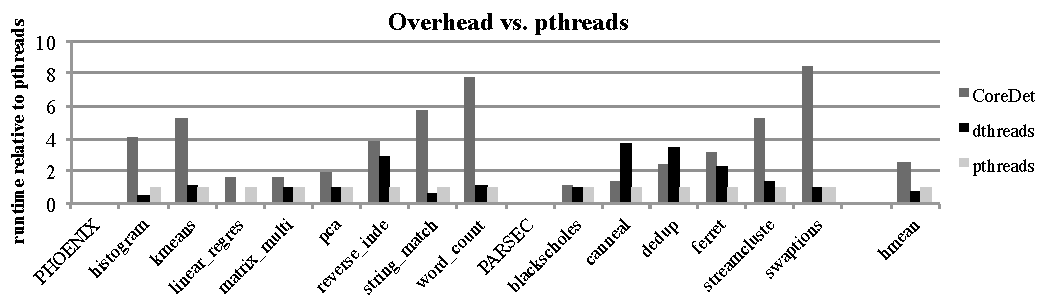
\includegraphics[width=6in]{dthreads/figure/overhead-figure}
\caption{Normalized execution time with respect to \pthreads{} and CoreDet(lower is better). For 9 of the 14 benchmarks, \dthreads{} runs nearly as fast or faster than \pthreads{}, while providing deterministic behavior.\label{fig:performance}}
}
\end{figure*}

\begin{table*}[!t]
\centering
\resizebox{\columnwidth}{!}{
\begin{tabular}{l|rr|l}
{\bf \small Benchmark} & $\frac{\mbox{\bf \small CoreDet}}{\mbox{\bf \small \pthreads{}}}$ & $\frac{\mbox{\small \bf \dthreads{}}}{\mbox{\small \bf \pthreads{}}}$ & {\bf \small Input} \\

\hline
{\bf \small histogram} &  $4.35\times$ & $0.52\times$ & {\it \small large.bmp} \\
{\bf \small kmeans} &  $5.05\times$ & $0.91\times$ & {\it \small -d 3 -c 1000 -p 100000 -s 1000} \\ 
{\bf \small linear\_regression}  & $1.50\times$ & $0.13\times$ & {\it \small key\_file\_500MB.txt} \\
{\bf \small matrix\_multiply}  & $1.55\times$ & $1.00\times$ & {\it \small 2000 2000 } \\
{\bf \small pca}  & $1.94\times$ & $1.03\times$ & {\it \small -r 4000 -c 4000 -s 100 } \\
{\bf \small reverse\_index} & $4.64\times$ & $2.73\times$ & {\it \small datafiles} \\
{\bf \small string\_match} & $5.95\times$ & $0.65\times$ & {\it \small key\_file\_500MB.txt} \\
{\bf \small word\_count} & $7.67\times$ & $1.09\times$ & {\it \small word\_100MB.txt} \\
{\bf \small blackscholes} & $1.13\times$ & $0.98\times$ & {\it \small 8 in\_1M.txt prices.txt} \\
{\bf \small canneal} & $1.00\times$ & $4.12\times$ &  {\it \small 7 15000 2000 400000.nets 128} \\
{\bf \small dedup} & $2.69\times$ & $3.39\times$ & {\it \small -c -p -f -t 2 -i media.dat output.txt} \\
{\bf \small ferret} & $3.69\times$ & $2.84\times$ & {\it \small corel lsh queries 10 20 1 output.txt} \\
{\bf \small streamcluster} & $4.87\times$ & $1.44\times$ &  {\it \small 10 20 128 16384 16384 1000 none output.txt 8} \\
{\bf \small swaptions} & $7.61\times$ & $0.95\times$ & {\it \small -ns 128 -sm 50000 -nt 8} \\
\hline
\end{tabular}
}
\caption{Benchmarks: normalized execution time and input parameters.\label{tbl:benchmarks}}
\end{table*}

For performance, We compare \dthreads{} to CoreDet
and \pthreads{}. Figure~\ref{fig:performance} presents these results graphically (normalized to the runtime of \pthreads{}); Table~\ref{tbl:benchmarks} provides detailed information about the normalized execution time and input parameters.

\dthreads{} outperforms CoreDet on 12 out of 14 benchmarks (running between 20\% and $12\times$ faster). For 9 benchmarks, \dthreads{} runs nearly the same as or better
performance than \texttt{pthreads}. Because \dthreads{} isolates updates in separate processes, it can improve performance by eliminating false sharing: since concurrent ``threads'' actually perform at different physical pages, there is no coherence traffic caused by false sharing between synchronization points. \dthreads{} eliminates catastrophic false sharing in the \texttt{linear\_regression} benchmark, allowing it to execute over $8\times$ faster than \pthreads{} and $12\times$ faster than CoreDet. The \texttt{string\_match} benchmark exhibits a similar, though less dramatic, false sharing problem, allowing \dthreads{} to run almost 56\% faster than \pthreads{} and $9\times$ faster than CoreDet. Two benchmarks, \texttt{histogram} and \texttt{swaptions}, also run faster with \dthreads{} than with \pthreads{} ($2\times$ and $6\%$, respectively; $2.7\times$ and $9\times$ faster than with CoreDet). We believe but have not yet verified that the reason is false sharing.

\dthreads{} runs substantially slower than \pthreads{} for 4 of the 14 benchmarks examined here. The \texttt{ferret} benchmark relies on an external library to analyze image files during the first stage in its pipelined execution model; this library makes intensive (and in the case of \dthreads{}, unnecessary) use of locks. Lock acquisitions and deacquisitions in \dthreads{} imposes higher overhead than ordinary \pthreads{} mutex operations. More importantly in this case, the intensive use of locks in one stage forces \dthreads{} to effectively serialize the other stages in the pipeline, which must repeatedly wait on these locks to enforce a deterministic lock acquisition order. The other three benchmarks (\texttt{canneal}, \texttt{dedup}, and \texttt{reverse\_index}) modify a large number of pages. With \dthreads{}, each page modification triggers a segmentation violation, a system call to change memory protection, the creation of a private copy of the page, and a subsequent copy into the shared space during commit phases. We note that CoreDet also substantially degrades performance for \texttt{dedup} and \texttt{reverse\_index}), so much of this slowdown may be inherent to any deterministic runtime system.

\subsection{Scalability}
\label{sec:scalability}

\begin{figure}
{\centering
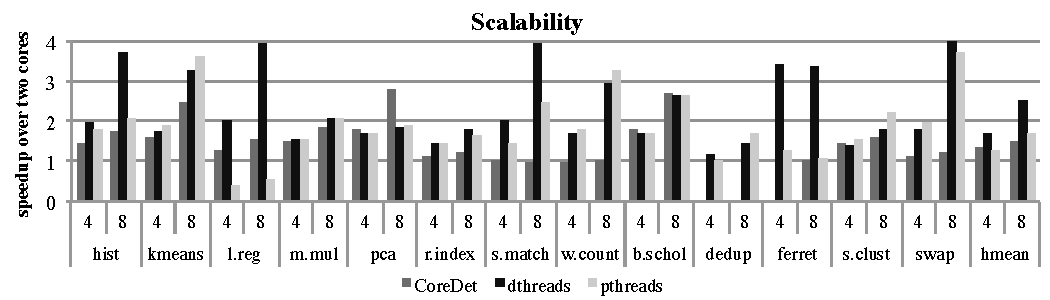
\includegraphics[width=6in]{dthreads/figure/scalability-figure}
\caption{Speedup of eight cores versus two cores (higher is better).  When possible to control with command line options, the number of threads was matched to the number of cores enabled.\label{fig:scalability}}
}
\end{figure}

To measure the scalability cost of running \dthreads{}, we ran two benchmark suite (excluding \texttt{canneal}) on the same machine with eight cores, four cores, and just two cores enabled.  Whenever possible without source code modifications, the number of threads was matched to the number of CPUs enabled.  We have found that \dthreads{} scales at least as well as \pthreads{} for 9 of 13 benchmarks, and scales as well or better than CoreDet for all but one benchmark. On average, \dthreads{} outperforms CoreDet by $3.5\times$.  Detailed results of this experiment are presented in Figure~\ref{fig:scalability} and discussed as follows.

\texttt{canneal} was excluded from the scalability experiment because this benchmark does more work when more threads are present, making the performance comparison between eight and two threads unfair.  \dthreads{} hurts scalability (relative to \pthreads{}) for four of the benchmarks: \texttt{kmeans}, \texttt{word\_count}, \texttt{dedup}, and \texttt{streamcluster}, although only marginally in most cases.  In all of these cases, \dthreads{} scales better than CoreDet.

\dthreads{} is able to match the scalability of \pthreads{} for three benchmarks: \texttt{matrix\_multiply}, \texttt{pca}, and \texttt{blackscholes}.  With \dthreads{}, scalability actually improves over \pthreads{} for 6 out of 13 benchmarks: \texttt{histogram}, \texttt{linear\_regression}, \texttt{reverse\_index}, \texttt{string\_match}, \texttt{ferret}, and \texttt{swaptions}.




\subsection{Performance Analysis}

\subsubsection{Benchmark Characteristics}

The data presented in Table~\ref{tbl:characteristics} are obtained from the executions running on all 8 cores.  Column 2 shows the percentage of time spent in serial phases.  In \dthreads{}, all memory commits and actual synchronization operations are performed in serial phases.  The percentage of time spent in serial phases thus can affect performance and scalability. Applications with higher overhead in \dthreads{} often spend a higher percentage of time in
serial phases, primarily because they modify a large number of pages that need to be committed during serial phases.

Column 3 shows the number of transactions in each application and Column 4 provides the average length of each transaction (ms).  Every synchronization, including locks, conditional variable, barriers, and thread exits, demarcate transaction boundaries in \dthreads{}.  For example, \texttt{reverse\_index}, \texttt{dedup}, \texttt{ferret}
and \texttt{streamcluster} perform numerous transactions whose
execution time is less than 1ms, imposing a performance penalty for these applications.  Benchmarks with longer (or fewer) transactions run almost the same speed as or faster than \texttt{pthreads}, including \texttt{histogram} or \texttt{pca}.  In \dthreads{}, longer transactions amortize the overhead of memory protection and copying over a longer period, thus reducing performance overhead.

Column 5 and 6 provides more detail on the costs associated with memory updates (the number and total volume of dirtied pages). From the table, it is clear why \texttt{canneal} (the most notable outlier) runs much slower with \dthreads{} than with \pthreads{}. This benchmark updates over three million pages, leading to large performance overhead caused by creating private copies, handling protection faults, and committing modifications on those pages to the shared memory mapping. 

\textbf{Conclusion: }
Most benchmarks examined here contain either a small number of transactions, thus having long running transactions, and modify a modest number of pages during execution. For these applications, \dthreads{} is able to amortize its overhead: by eliminating false sharing, it can even run faster than \pthreads{}. However, for the few benchmarks that perform numerous short-lived transactions, or modify a large amount of pages, \dthreads{} can introduce substantial overhead.


\begin{table*}[!t]
\centering
\resizebox{\columnwidth}{!}{
\begin{tabular}{l|rrrrr}
& {\bf \small Serial Phase} & {\bf \small Transactions} & {\bf \small TransLength} & {\bf \small DirtyPages} & {\bf \small DirtyPages}
\\
{\bf \small Benchmark} & {\bf \small (\% of time)} & {\bf (\#)} & {\bf \small (ms)} & {\bf \small (\#)} & {\bf \small (GB)}\\
%\hline
%\multicolumn{6}{|c|}{\emph{Phoenix}} \\
\hline
\small \textbf{histogram} & 0 & 23 & 15.47 & 29 & 0 \\
\small \textbf{kmeans} & 0 & 3929 & 3.82 & 9466 & 0.04\\
\small \textbf{linear\_regression} & 0 & 24 & 23.92 & 17 & 0\\
\small \textbf{matrix\_multiply} & 0 & 24 & 841.2 & 3945 & 0.02\\
\small \textbf{pca} & 0 & 48 & 443 & 11471 & 0.04 \\
\small \textbf{reverseindex} & 17\% & 61009 & 1.04 & 451876 & 1.72\\
\small \textbf{string\_match} & 0 & 24 & 82 & 41 & 0 \\
\small \textbf{word\_count} & 1\% & 90 & 26.5 & 5261 & 0.02\\
%\hline
%\multicolumn{6}{|c|}{\emph{PARSEC}} \\
%\hline
\small \textbf{blackscholes} & 0 & 24 & 386.9 & 991 & 0\\
\small \textbf{canneal} & 26.4\% & 1062 & 43 & 3606413 & 13.75\\
\small \textbf{dedup} & 31\% & 45689 & 0.1 & 356589 & 1.36\\
\small \textbf{ferret} & 12.3\% & 484127 & 0.05 & 844184 & 3.21 \\
\small \textbf{streamcluster} & 18.4\% & 130001 & 0.04 & 131992 & 0.50\\
\small \textbf{swaptions} & 0 & 24 & 163 & 867 & 0\\
\hline
\end{tabular}
}
\caption{Benchmark characteristics.\label{tbl:characteristics}}
\end{table*}

\subsubsection{Performance Impact Analysis}
We further evaluate the performance impact of two important components of \dthreads: deterministic synchronization (sync-only) and memory protection(prot-only).

\emph{Sync-only}: This configuration enforces a deterministic synchronization order. However, memory protection is not enabled so all ``threads'' (actually processes) access the shared memory directly. We want to use this to show the performance impact of load imbalance, caused by synchronization based scheduling.

\emph{Prot-only}: This configuration runs threads in isolation, and commits at synchronization points. The order of synchronization and memory commits are non-deterministic. This configuration eliminates false sharing, but also introduces the performance overhead of isolation and memory commits. In order to guarantee correct execution, we replaced those synchronizations as corresponding cross-processes synchronizations. The lazy twin creation and single-threaded execution optimizations are disabled here because they are unsafe without deterministic synchronization. Thus, this configuration actually evaluates the performance of the \sheriff{} framework. 


\begin{figure*}[!t]
{\centering
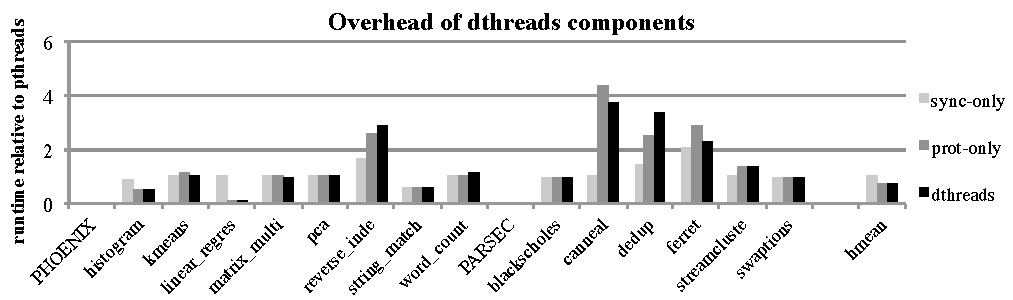
\includegraphics[width=6in]{dthreads/figure/perfeffect}
\caption{Normalized execution time with respect to \pthreads{} (lower is better) for three different configurations. 
\label{fig:perfanalysis}}
}
\end{figure*}

The performance results of these two configurations are shown in Figure~\ref{fig:perfanalysis} and discussed in the following.

\begin{itemize}

\item
The \texttt{reverse\_index}, \texttt{dedup} and \texttt{ferret} benchmarks show significant load imbalance under {\it sync-only} configuration. Additionally, these benchmarks introduces significant overhead with {\it prot-only} configuration because of a large number of transactions there. That explains why \dthreads{} doesn't have good performance on these benchmarks.

\item
The \texttt{string\_match} benchmark shows performance improvement with {\it sync-only} configuration. The exact reason is not clear, may be due to our custom memory allocator (described in Section~\ref{sec:customheap}) that eliminates false sharing problems. 

\item
The \texttt{linear\_regression}, \texttt{histogram} and \texttt{swaptions} benchmarks improve performance with {\it prot-only} configuration. The memory isolation mechanism eliminates false sharing problems inside and contributes to the performance speedup.

\item
Normally the performance of \dthreads{} is not better than the performance of the {\it prot-only} configuration. However, both \texttt{ferret} and \texttt{canneal} run faster with determinism enabled (under \dthreads{}). Both are benefited from specific optimization described in Section~\ref{sec:dthreads-optimization}. \texttt{ferret} benefits from the \emph{single-threaded-execution}. The performance improvement of \texttt{canneal} is coming from the shared twin pages for all threads in parallel phases.

\end{itemize}







\section{Discussion}
\label{sec:discussion} All DMT systems must impose an order on updates to shared memory and synchronization operations.  The
mechanism used to isolate updates affects the limitations and performance of the
system.  \dthreads{} represents a new point in the design space for DMT systems with some inherent advantages and limitations as follows.

\subsection{Design Tradeoffs} 

CoreDet and \dthreads{} both use a combination of
parallel and serial phases to execute programs deterministically.  These two systems take different approaches during parallel phases, as
well as the transitions between phases:

\textbf{Memory isolation:} 
CoreDet orders updates to the shared memory by
instrumenting all memory accesses that could reference shared data. Synchronization operations and updates to shared memory must be performed in serial phases, unless those updates are performed by owners of a block, which can issued in parallel phases. This approach results in high instrumentation overhead during parallel phases, but incurs no additional overhead when exposing updates to the shared state since they are shared already.

\dthreads{} takes an alternate approach: updates proceed at full speed, but are isolated using hardware-supported virtual memory.  When a serial phase is reached, these updates are committed to the shared state in a deterministic order, with
the help of the twinning-and-diffing mechanism described in Section~\ref{sec:twinning-and-diffing}.

A pleasant side-effect of \dthreads{} is the elimination of false sharing. Because threads work in separate address spaces, there is no need to keep caches coherent between threads during parallel phases.  For some programs, this results in a performance improvement as large as $7\times$ when compared to
\pthreads{}.

\textbf{Phases:} 
CoreDet employs a quantum-based scheduler: after the specified number of instructions is executed in a parallel phase, the scheduler transitions to a serial phase. This approach bounds the waiting time for any thread that are blocked to the quantum, reducing the load imbalance problem.  One drawback of this approach is that transitions to a serial phase do not correspond to static program points.  Any changes of code and input will result in a new, previously-untested schedule.

Transitions between phases are static in \dthreads{}.  Any synchronization operation will result in a transition to a serial phase, and a parallel phase
will resume once all threads have finished their critical sections.  This makes \dthreads{} susceptible to delays due to load imbalance between threads, but results in more robust determinism.  With \dthreads{}, only the order of synchronization operations affects the schedule. For most programs, this means that different inputs, and even many code changes, will not change the schedule produced by \dthreads{}, as long as those changes won't affect the order of synchronizations.

\subsection{Limitations}
\label{sec:limitations}

This section analyzes some key limitations of \dthreads{} that restrict its ability to run certain programs, limit the extent of determinism it can guarantee, or potentially affect performance.

\textbf{Unsupported programs: }
\dthreads{} supports programs that
use the pthreads library, but does not support programs that
bypass it by using their own ad hoc synchronization operations, such as those that use atomic operations. However, the upcoming C++0X standard includes a library interface for atomic operations~\cite[pp. 1107--1128]{c++0xstandarddraft}, and a future version of \dthreads{} could intercept these library calls and treat them as synchronization points. While ad hoc synchronization is a common practice, it is also a notorious source of bugs; Xiong et al.\ show that 22--67\% of the uses of ad hoc
synchronization lead to bugs or severe performance issues~\cite{ad-hoc-considered-harmful}.

Currently, \dthreads{} also does not share the stack
across threads, so any updates to stack variables are only locally visible, which could cause a program to fail. However, communicating across different threads using stack variables  is extremely error-prone and generally deprecated, making this a rare coding practice.

\textbf{External determinism: }
While \dthreads{} provides internal determinism, it does not guarantee determinism when a program's behavior depends on external sources of non-determinism, such as system time or I/O events. Incorporation of \dthreads{} in the dOS framework, an OS proposal that enforces system-level determinism, would provide full deterministic execution, although this remains future work~\cite{deterministic-process-groups}.

\textbf{Runtime performance: }
Section~\ref{sec:evaluation} shows that \dthreads{} can provide high performance for a number of applications; in fact, for the majority of the benchmarks examined, \dthreads{} matches or even exceeds the performance of \pthreads{}. However, \dthreads{} could occasionally degrade performance, sometimes substantially. One way it could do so would be to exhibit an intensive use of locks (that is, acquiring and releasing locks at very high frequency), which are much more expensive
in \dthreads{} than in \pthreads{}. However, because of its determinism guarantees, \dthreads{} could allow programmers to greatly reduce their use of locks, and thus improve performance. Other application characteristics, also explored in Section~\ref{sec:performance}, can also impair performance
with \dthreads{}.


%  Since Surprise locking inside libraries. Not a limitation \emph{per
%  se} but definitely an issue that could surprise programmers.

% Draft can be downloaded from http://www.open-std.org/jtc1/sc22/wg21/docs/papers/2010/n3126.pdf.
%Fine once they are library calls, as they are in gcc and in the upcoming C++0X standard (cite!), since then we can intercept them.

\textbf{Memory consumption: }
Because \dthreads{} creates private, per-process copies of modified pages between commits, it can increase a program's memory footprint by the number of modified pages between synchronization points. This increased footprint does not seem to be a problem in practice, both because the number of modified pages is generally far smaller than the number of pages read, and because it is transitory: all private pages are relinquished to the operating system (via \texttt{madvise()}) at the end of every commit operation.

\textbf{Memory consistency:} 
\dthreads{} provides a form of release consistency for parallel programs, where updates are exposed at static program points. 
CoreDet's DMP-B mode also uses release consistency, but the update points depend on when the quantum counter reaches zero.  To the best of our knowledge, \dthreads{} cannot produce an output that is not possible with \pthreads{}, although for some cases it will result in unexpected outputs.  But the same unexpected output will be produced on every run
with \dthreads{}, making it easier for developers to track down the source of the problem than with \pthreads{}.




\chapter{Precise Detection and Automatic Mitigation of False Sharing}
\label{chapter:sherifftools}

False sharing is a well-known performance issue~\cite{falseshare:effect, falseshare:Analysis}. We have discussed this problem in Section~\ref{sec:falsesharingproblems}. 

Detecting false sharing requires tools support. Existing tools share a similar shortcoming, where they can not pinpoint the exact place with false sharing problems, leaving the burden of finding actual places to programmers. Besides that, existing tools suffer from one or more different shortcomings.  Simulation based approaches ~\cite{falseshare:simulator} and binary instrumentation based approaches~\cite{falseshare:binaryinstrumentation1, falseshare:binaryinstrumentation2} normally introduce very significant performance overhead, slowing down the execution over $100\times$. Hardware performance counter based approaches generally provide much better performance, but they cannot differentiate false sharing from true sharing problems~\cite{detect:ptu, detect:intel}.

We provide two systems, \SheriffDetect{} and \SheriffProtect{}, to tackle with false sharing problems, based on the \sheriff{} framework that discussed in Section~\ref{sec:sheriffframework}. \Sheriff{} is a drop-in replacement of the standard \pthreads{} library, but providing ``per-thread'' protection and isolation mechanism. \SheriffDetect{} detects false sharing problem accurately (without false positives) and precisely, by pointing out the exact places with false sharing problems. It is also very efficient, only introducing 20\% performance overhead.  \SheriffProtect{} automatically tolerate false sharing problems when rewriting an application to resolve false sharing is infeasible or impractical. The reasons can be caused by either source code is unavailable, or padding data structures would degrade performance because of reduced cache utilization and/or increase memory footprint.


%\section{\sheriff{} Framework}
%\input{sheriff/overview}

\section{Detecting False Sharing}
\label{sec:detectfalseshare}

This section first describes the basic idea of detecting false sharing. 

\subsection{Basic Idea}
\label{sec:detectionidea}
False sharing occurs when more than two threads concurrently access independent data within the same cache line, at least one of them are writes. False sharing does not necessarily cause performance problems. It can greatly degrade performance only when those accesses, caused by threads running on different cores with separate cache, actually cause a big number of cache invalidations. This is our \textbf{basic observation}. 

Generally, there are two known approaches to know how many cache invalidations actually occurring on a specific cache line, but they all suffer different shortcomings. 

The first approach relies on the underlying hardware, called as ``hardware-based approach''. We may rely on specific hardware performance counters, existing in some special hardware but not all, to know this information. But we cannot have thorough information about cache invalidations since existing mechanisms are based on sampling, which can lost a lot of information. Also, a tool based on this approach cannot apply to a different hardware that do not have specific hardware support. 

The second approach is to simulate the cache activity on different cache lines. To do that, we have to know all hardware-related information, including cache hierarchy, cache capacity and cache eviction rule, and the relationship between a thread and a specific core (that is hard to match actual situation). Even worse, simulation-based approaches are normally very slow and cannot be generalized to an execution running on a different hardware environment. 

To avoid these problems, we provide a software-only and generalized approach that can only rely on memory access history of each cache line, which is used by both \SheriffDetect{} and \Predator{} (discussed in Section~\ref{chapter:preditor}). Our approach is based on two conservative assumptions.
  
{\it First assumption:} 
All threads are running on different cores, with separate caches. Using this assumption can avoid knowing actual hardware cache hierarchy and the running situation between a thread and different cores. Although in a particular execution, two threads may run on the same core, thus reducing the effect of possible false sharing problems. Assuming that two threads are running on different cores can always represent a worst-case scenario that can happen in future executions. Thus, this assumption is very conservative, helping report any possible false sharing problem. 

{\it Second assumption:} 
A cache entry is never evicted from its private cache by cache eviction, meaning that all caches have infinite capacity. This assumption allows us to compute a cache invalidation without considering whether this entry is still in the cache or not. 

These two assumptions together allow us to compute cache invalidations based on memory accesses only. Based on these assumptions, we have the following {\bf observation}: there is a cache invalidation if a thread writes a cache line after another thread's access on the same cache line. Because the last thread accessing this cache line creates a copy of the same cache line on its running core's private cache (first assumption) and holds this copy(second assumption), this write operation definitely causes a cache invalidation, which invalidates the data copy on the core accessed by last thread. 


\begin{figure}[!t]
\centering
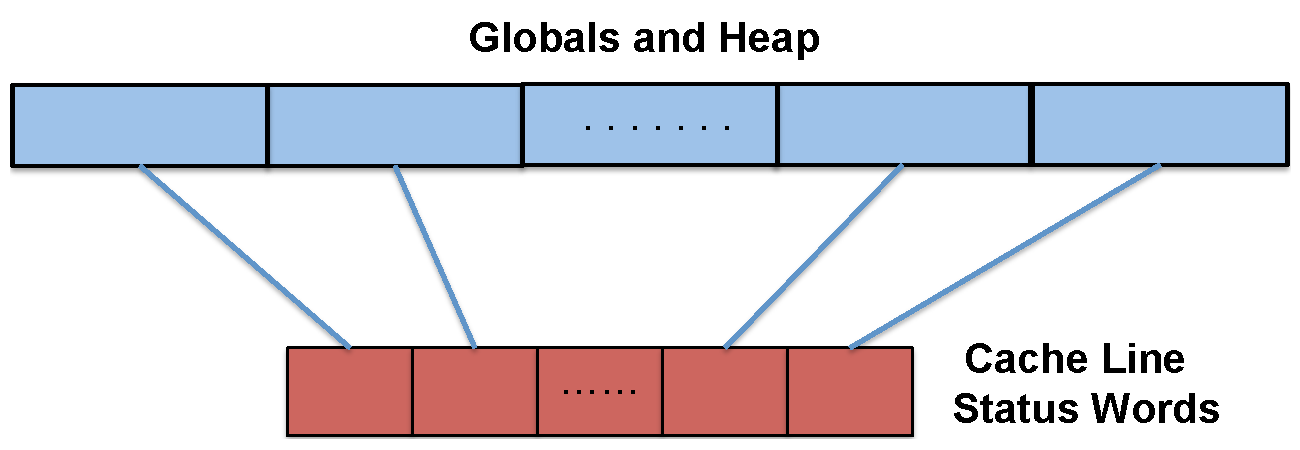
\includegraphics[width=6in]{fig/cachelinestatuswords}
\caption{
To detect false sharing, each cache line of the globals and heap maintains a cache line status word, which is updated on each memory access. \label{fig:cachelinestatusword}}
\end{figure}


To locate cache lines with a big number of cache invalidations, we maintain a cache line status word for each cache line in the globals and heap, shown in Figure~\ref{fig:cachelinestatusword}. We share a similar mechanism as another concurrent work of Zhao et.al. ~\cite{qinzhao}. 
However, the detailed implementation is totally different. Zhao et.al. utilize the detailed ownership bitmap to track those cores that have a duplicate copy of data, which can even track how many cache invalidations may happen in a write operation. However, their design cannot be easily scaled to more than 32 threads, requiring more memory overhead caused by more bits and more checking performance overhead. Also, their approach misses one important factor -- how many cache invalidations happening on a specific cache line. Without this information, it is impossible to pinpoint false sharing problems that can cause performance problems.
Our approach overcomes these shortcomings, by only tracking the last thread index and the number of cache invalidations.  Thus, we can rank the seriousness of false sharing problems based on the number of cache invalidations.
 

\subsubsection{Accurate Detection}
\label{sec:accuratedetect}
Accurate detection implies that we only report those false sharing problems that can cause performance problems. We employs the following mechanisms to avoid false positives.

First, we only report false sharing problems with a big number of cache invalidations, larger than a pre-defined but changeable threshold, thus can potentially cause performance problems. Utilizing the number of cache validations as an indicator avoids the problem of some existing tools, like PTU~\cite{detect:ptu, detect:intel}. PTU aggregates memory accesses without considering memory access interleaving, which  can report some cases that has a big number of memory accesses but without many cache invalidations. 

Second, we can differentiate false sharing from true sharing since true sharing can also cause cache invalidations. To do this, Zhao et.al. update bitmaps for every read and write in order to precisely determine whether an invalidation is related to a false sharing or a true sharing ~\cite{qinzhao}. However, this approach brings scalability problem that can not scale to more threads, bringing more memory overhead. We achieve the same target differently: we do not differentiate false sharing from true sharing during normal executions, but only track word-level accesses information: how many reads or writes are issued by which thread, where a word accessed by multiple threads is as ``shared''. This design lets us accurately distinguish false sharing from true sharing in the reporting phase, while do not have the scalability issue. It also helps diagnose where actual false sharing occurs when there are multiple fields or multiple objects in the same cache line, as this can greatly reduce the manual effort required to fix the false sharing problems.

  
Third, we can avoid pseudo false sharing (false positives) caused by memory reuses.  We intercept those memory allocations and deallocations, update information at memory deallocations for those objects without false sharing problems; heap objects involved in false sharing are never reused so that they can be reported in the end or on demand.


\subsubsection{Precise Detection}
\label{sec:precisedetect}

Precise detection implies that we can precisely point out where the problem is. Thus, programmers can leverage on that to identify and correct false sharing problems.

For global variables, we identify the name of global variables involving in false sharing problems, by looking up corresponding debug information. For heap objects, we report the callsite of those memory allocations by presenting the line of source code. In order to capture the origins of heap objects, we intercept those intercepting memory allocations and deallocations and use different ways to get callsite information, which are discussed in Section~\ref{sec:sheriffcallsite} and Section~\ref{sec:predatorcallsite}.

To help programmers precisely identify culprits of performance problem, we also present word-level accesses information so that the exact variables or fields that cause performance problems can be determined precisely. 

\subsubsection{Flexible Reporting}
\label{sec:flexiblereport}

We provide two different ways to report those false sharing problems. Normally, we can report those false sharing problems in the end of a program. However, this way does not work for those long-running applications. Thus, we provide a on-demand reporting way. User can send a specified signal to those applications that are installed with our tool. By intercepting those signals, we can report false sharing problems on demand.

In order to find out those cache lines with false sharing problems, we scan cache line status words of all memory, including the globals and heap, and only report those false sharing problems that can possibly cause performance problems, with the number of cache invalidations larger than a pre-defined but adjustable threshold.

\subsection{Detailed Implementations}

\label{sec:sheriffdetect}
\SheriffDetect{} relies on the \sheriff{} framework to track memory writes, thus detecting the write-write type of false sharing problems.  

%%% Tongping Liu
\subsubsection{Tracking Memory Accesses}
\label{sec:memoryaccesses}

\begin{figure*}[!t]
\centering
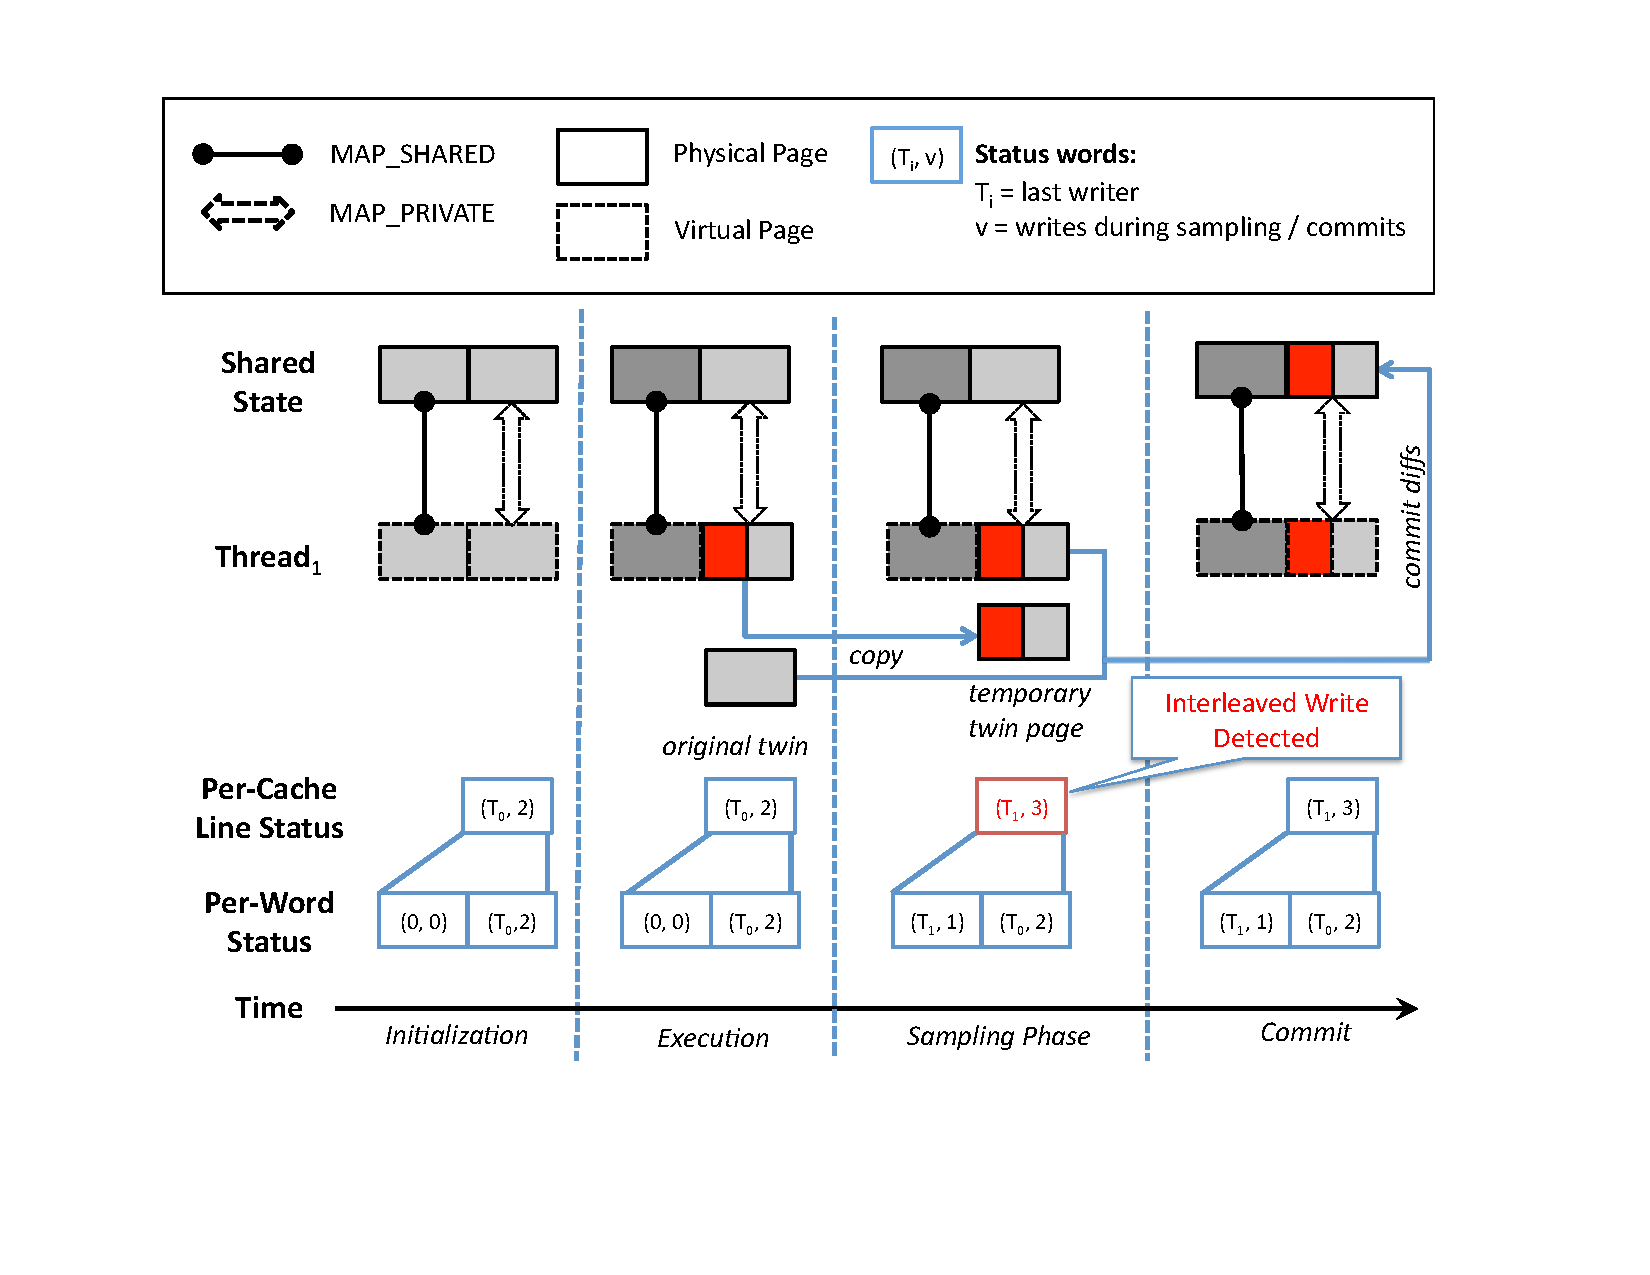
\includegraphics[width=6in]{sheriff/figure/sheriffdetective.pdf}
\caption{
Overview of \SheriffDetect{}’s operations. \SheriffDetect{} extends \Sheriff{} with sampling, per-cacheline status arrays, and per-word status arrays. For clarity of exposition, the diagram depicts just one cache line per page and two words per cache line.\label{fig:sheriffdetect}}
\end{figure*}

As discussed in Section~\ref{sec:detectionidea}, we can detect cache invalidations only based on memory accesses: for every memory access, we check recent memory access history, update the number of cache invalidations if possible, and update corresponding memory access history. 
Base on our observation, if the current access is a write, and other threads have accessed this cache line since last invalidation, then there is a cache invalidation. 
The \sheriff{} framework isolates executions from different threads, only commits those changes of different threads to the shared mapping at synchronization boundaries. Thus, by comparing a ``working'' page against its ``twin'' page,  \sheriffDetect{} can discover those accumulative memory writes  that occurred in the last transaction.  

However, if a transaction is long-running, finding memory changes at the end of every transaction is not enough 
to find those false sharing problems happening in the middle of a transaction. For example, the \texttt{linear\_regression} benchmark (described in Section~\ref{sec:evaluation}), 
degrading the performance by more than $10\times$ because of its false sharing problem, only has a single transaction per thread. 

In order to detect memory writes in the middle of an transaction, \SheriffDetect{} employs a sampling mechanism, employing the timer mechanism of the underlying operating system. 
We utilize the \texttt{alarm} library API to generate a periodical alarm to our detection system: by handling the \texttt{SIGALRM} signal, \SheriffDetect{} tracks memory writes accumulatively in the current period using the twinning-and-diffing mechanism (section~\ref{sec:twinning-and-diffing}). To do this, \SheriffDetect{} also keeps and updates a ``temporary twin'' page at every alarm interval, by simply copying from its ``working'' page. The difference between a ``working'' page and its ``temporary'' page implies those memory writes happening in the current sampling period. 

Currently, \SheriffDetect{} samples memory accesses of each thread at every 10 microsecond, which is  adjustable in our implementation. More frequent sampling may uncover more false sharing problems, but at the cost of increasing performance overhead. The tradeoff between effectiveness and performance overhead is further discussed and evaluated in Section~\ref{sec:results-sampling-overhead}. 

\subsubsection{Tracking Cache Invalidations}
\label{sec:invalidation}
As the discussion in Section~\ref{sec:detectionidea}, \SheriffDetect{} tracks and reports those cache lines with a big number of cache invalidations, which may cause serious performance problems. 

In order to track cache invalidations, \SheriffDetect{} introduces a cache line status word for every cache line of the globals and heap, showed in Figure~\ref{fig:cachelinestatusword}.  \SheriffDetect{} introduces two fields for every cache line status word, the last thread writing to this cache line and the number of cache invalidations of this cache line. 
Every time, when \SheriffDetect{} tracks a memory write, either at the end of each transaction or during the sampling timer handler, it updates these two fields correspondingly. Based on the assumptions described in Section~\ref{sec:detectionidea}, \SheriffDetect{} increments the number of cache invalidations when there is a write from a different thread and changes the last thread to the current thread (by recording thread id). To avoid using lock, \SheriffDetect{} updates those counters using atomic primitives. Since we base on thread id to identify whether there is a cache invalidation, without keeping track of detailed ownership id, this approach can scale up to any number of threads.   

\subsection{Optimizations}

\SheriffDetect{} employs the following optimizations in order to reduce its performance overhead. 

\paragraph{Getting Callsite Information.}
\label{sec:sheriffcallsite}

\SheriffDetect{} intercepts memory allocation operations in order to collect callsites for every heap object. To reduce the performance overhead, \SheriffDetect{} does not use the \texttt{bracktrace()} function call, but identify the callsite by analyzing the return or frame address using GCC extensions. However, this can not work on applications without debugging information. 

\paragraph{Reducing timer overhead.}
As explained in Section~\ref{sec:memoryaccesses}, \SheriffDetect{} uses a sampling mechanism to track cache invalidations. To reduce the performance overhead caused by by handling those alarm signals, \SheriffDetect{} activates sampling only when the average transaction time is larger than a pre-defined threshold (currently 10 milliseconds). \SheriffDetect{} uses an exponential moving average to track the average transaction time ($\alpha = 0.9$). This optimization does not significantly reduce the possibility of finding false sharing, since \SheriffDetect{} can track those accumulative writes inside every short transaction by checking only at the end of transactions.

\paragraph{Sampling to find shared pages.} 
If an application has a large number of transactions or a large memory footprint, the overhead of handling page protection can dominate the total running time.
To reduce the number of pages that should be tracked, \SheriffDetect{} leverages a
simple insight: if two threads can falsely share (write-write share) a cache line, then they must simultaneously write to the same page containing this cache line. 
Leveraging on this insight, \SheriffDetect{} only tracks those pages written by multiple threads. 

In order to identify those shared pages, \SheriffDetect{} is based on the following assumption: if objects on a page are frequently falsely shared, the corresponding page must also be frequently shared; thus, even relatively infrequent sampling on memory accesses can reveal the shared relationship. \SheriffDetect{} currently samples the first 50 out of every 1,000 periods (one period equals one transaction or one sampling interval). At the beginning of each sampling period, all memory pages are made read-only so that any
writes to each page will be detected. Upon finding a page that is shared across multiple threads, \SheriffDetect{} tracks all memory accesses happening on this page, thus possibly finding any false sharing inside this page. 

By using this sampling mechanism, those pages, with sharing status unknown, impose no protection overhead at all. \sheriffDetect{} only pays protection overhead for those shared pages outside the sampling period, instead of all memory pages. 

\subsection{Limitation}
\label{discussion:faultofdetect}

Unlike previous tools, \SheriffDetect{} reports no false positives, differentiates true sharing from false sharing, and avoids false positives caused by the reuse of heap objects. 

However, \SheriffDetect{} can under-report false sharing instances in the following situations:

\paragraph{Single writer.}
False sharing usually involves concurrent updates from multiple threads. But it can also arise when there is exactly one thread writing to part of a cache line while other threads read from this cache line. 
Because \sheriffdetect{} can only track writes, it cannot detect this single-writer false sharing, missing some false sharing problems. 

\paragraph{Heap-induced false sharing.}  
\sheriff{} replaces the standard memory allocator with one that, like the Hoard allocator, avoids most heap-induced false sharing. \sheriff{}'s memory allocator (like Hoard), carves memory into page-sized chunks; each thread allocates from its own set of chunks, and the allocator never splits cache lines across threads. Because \SheriffDetect{} uses a different custom memory allocator, it cannot detect false sharing that is caused by using the standard memory allocator. Since it is straightforward to deploy Hoard or a similar allocator to avoid heap-induced false sharing, this limitation is not a problem in practice.

\paragraph{Misses due to sampling.}  Since it uses sampling to find shared pages, \SheriffDetect{} may fail to track those pages that written in the middle of sampling intervals. We hypothesize that false sharing instances that affect performance are unlikely to perform frequent writes exclusively during that time, and so are unlikely to be missed.


\section{Tolerating False Sharing}
\label{sec:sheriffprotect}
While \SheriffDetect{} can effectively find those false sharing problems of multithreaded programs, it is sometimes difficult or impossible to fix them. For example, padding memory to avoid false sharing may even slowdown the performance because of excessive memory consumption or reducing cache utilization~\cite{qinzhao}. Also, time constraints or unavailable source code may prevent the fixes. 

Based on the \sheriff{} framework, we provide the second tool, \SheriffProtect{}, to automatically boost the performance for multithreaded applications with false sharing problems, without programmer intervention.  

\SheriffProtect{} borrows the insight initially introduced by Dubois et.al.~\cite{Dubois:1991:DCE:125826.125941}: {\it delaying updates avoids false sharing}. Because \Sheriff{} replaces threads with processes, executions of different threads are actually isolated from each other. Thus, different ``threads'' (processes) actually access different physical pages (and cache lines), when originally they are accessing the same cache line in the multithreading environment. This helps avoid false sharing problems. 

However, simply using the \sheriff{} framework introduces excessive performance overhead because of the following reasons: 

\begin{itemize}
\item
The overhead of protecting and committing all pages may be too high. As we already know in Section~\ref{sec:sheriffframework}, \sheriff{} has to commit all local changes of different threads  to the shared mapping at the end of every transaction (synchronization points) in order to achieve the shared memory semantics. 

\item
If the length of a transaction is short, the overhead of protecting and committing pages in the \sheriff{} framework can be easily higher than the performance benefit by tolerating possible false sharing problems inside. Thus, there is no benefit to tolerate false sharing problems for short-running transactions. 

\end{itemize}

\sheriffprotect{} provides two corresponding mechanisms to avoid these possible overhead. 

\emph{Selective Protection.} 
\SheriffProtect{} only prevents false sharing on small objects, with size less than 1024 bytes. All large objects are mapped shared and are never protected, thus can not tolerate false sharing problems caused by these large objects. We expect  small objects to be a likely source of false sharing because more of them can fit on a cache line. Also, for large objects, the cost of protecting and committing changes can be bigger than the benefit of tolerating possible false sharing problems inside. 

\emph{Adaptive Prevention.}
\SheriffProtect{} employs a simple adaptive mechanism: it only isolates threads' executions if the average transaction length is large than a pre-set threshold. \SheriffProtect{} keeps track of the length of each transaction and uses a exponential weighted averaging ($\alpha = 0.9$) to calculate the average transaction length. If the average transaction length falls below an established threshold, \SheriffProtect{} switches to the shared mappings for all memory and does no further page protections. As long as transactions remain too short, 
 without any benefit to tolerate false sharing problems inside, the protection mechanisms remain switched off. If the average transaction length rises back above the threshold, \SheriffProtect{} re-establishes private mappings and page protections, thus avoiding possible false sharing to achieve better performance.

\section{Experimental Evaluation}
\label{sec:evaluation}

We perform all of our evaluations on a quiescent dual processor (totally 8 cores) system with 8GB of RAM. Each processor is a 4-core 64-bit Intel Xeon, running at 2.33 GHz with a 4MB L2 cache. For compatibility reasons, we compile all applications to a 32-bit target using the GCC compiler. All performance data is the average of ten runs, excluding the maximum and minimum values.

The evaluation answers the following questions:

\begin{itemize}
\item How effective is \sheriffdetect{} at finding false sharing and guiding programmers to their resolution? (Section~\ref{sec:effecteval})
\item What is \sheriffdetect{}'s performance overhead? (Section~\ref{sec:results-runtime-overhead})
\item How sensitive is \sheriffdetect{} to different sampling rates? (Section~\ref{sec:results-sampling-overhead}) 
\item How effective does \sheriffprotect{} mitigate false sharing? (Section~\ref{sec:protectperformance})
\end{itemize}

\subsection{Detection Effectiveness}

\label{sec:effecteval}

This section evaluates whether \sheriffdetect{} can be used to find false sharing problems, both in synthetic test cases and in actual applications.

We developed a range of microbenchmarks that exemplify different situations related to false sharing. We evaluate these benchmarks on both \SheriffDetect{} and Intel's Performance Tuning Utility(PTU v3.2), the previous state-of-the-art work of false sharing detection. 

Detection results are shown in Table~\ref{table:microbenchmarks}. \sheriffdetect{} only reports those false sharing instances that can possibly affect performance, while correctly ignores those cases without performance impact.
PTU has false alarms/positives.  It does not track access patterns, which reports false positives for those non-interleaved accesses. Also, PTU does not track memory deallocations, thus it can not filter out those pseudo false sharing caused by memory reuse. \sheriffdetect{} avoids all of these problems and reports false sharing problems correctly. 


\begin{table}
\centering
\resizebox{\columnwidth}{!}{
\begin{tabular}{l|l|l|l}
\hline
{\bf \small Microbenchmark} & {\bf \small Perf Sensitive } & {\bf \small \sheriffdetect{} } & {\bf \small PTU } \\
\hline

\small \textbf{False Sharing (adjacent objects)} & YES & \cmark{} & \cmark{} \\
\small \textbf{False Sharing (same object)} & YES & \cmark{} & \cmark{} \\
\hline
\small \textbf{True Sharing} & NO & & \\
\small \textbf{Non-interleaved False Sharing} & NO & & \xmark{}\\
\small \textbf{Heap Reuse(no sharing)} & NO & & \xmark{}\\
\hline
\end{tabular}
}
\caption{False sharing detection results using PTU and \sheriffdetect{}. \sheriffdetect{} correctly reports only actual false sharing instances that have performance impact;
\cmark{} indicates a correct report and \xmark{} indicates a false alarm. 
\label{table:microbenchmarks}}
\end{table}

We further evaluate \SheriffDetect{} and PTU on two widely-used benchmark suites, Phoenix~\cite{phoenix-hpca} and PARSEC~\cite{parsec}. We use the simlarge inputs for all applications of PARSEC. For Phoenix, we choose available parameters that allow the programs to run as long as possible. We were unable to successfully compile \texttt{raytrace} and \texttt{vips}, and \sheriff{} is currently unable to run \texttt{x264}, \texttt{bodytrack}, and \texttt{facesim}. \texttt{Freqmine} currently can not support \pthreads{}. Thus, those benchmarks are excluded here. 
 
\begin{table}
\centering
\begin{tabular}{l|r|r}
\hline
{\bf \small Benchmark} & {\bf \small PTU} & {\bf \small \sheriffdetect{}}\\
 & {\# Lines} & {\# Objects}\\
\hline
\small \textbf{kmeans} & 1916 &  2 \\
\small \textbf{linear\_regression} & 5 & 1 \\
\small \textbf{matrix\_multiply} & 468 & 0\\
\small \textbf{pca} & 45 & 0 \\
\small \textbf{reverseindex} & N/A & 5 \\
\small \textbf{word\_count} & 4 & 3\\
\hline
\small \textbf{canneal} & 1 & 1 \\
\small \textbf{fluidanimate} & 3 & 1 \\
\small \textbf{streamcluster} & 9 & 1\\
\small \textbf{swaptions} & 196 & 0\\
\hline
\small \textbf{Total} & 2647 & 14\\
\hline
\end{tabular}
\caption{Overall detection results of PTU and \sheriffdetect{} on Phoenix and PARSEC benchmark suites. We only list those benchmarks that at least one of tools reports false sharing problems. For PTU, we show how many cache lines are marked as falsely shared. For \sheriffdetect{}, we show how many objects are reported by \sheriffdetect{} (with cache invalidations larger than 100). The item marked as ``N/A'' means that PTU fails to show results because it runs out of memory.
\label{table:fsdetection}}
\end{table}


The overall results are shown in Table~\ref{table:fsdetection}. PTU reports that 2647 cache lines may exist false sharing problems. \sheriffdetect{} reveals that seven out of sixteen evaluated benchmarks have false sharing problems. Totally, only 14 objects are reported, but only 4 of them shows a big number of cache invalidations, thus needs to be fixed. 

Several reasons contribute to the number difference between these two approaches. First, PTU reports cache lines involving in false sharing, while \SheriffDetect{} only reports objects. If an object has a size larger than the size of cache line, PTU can report multiple times, one on each cache line. Second, PTU reports multiple times if a heap object, with the same allocation site, is allocated multiple times, while \SheriffDetect{} only reports once. Third, PTU may report false positives since it does not track interleaved accesses and overrates the problems caused by heap reuses. 

We manually fix these four false sharing problems based on reports of \SheriffDetect{}, and show the performance gains after fixes in Table~\ref{table:perfafterfix}. To explain why performance improvement are different, we also examine the maximum possible updates that can occur on a false sharing object, although the actual number of interleaved accesses depends on actual scheduling. For example, \texttt{linear\_regression} has the largest updates, thus causing the most serious performance problem. 

\begin{table}
\centering
\begin{tabular}{l|r|r}
\hline
{\bf \small Benchmark} & {\bf \small Performance Improvement} & {\bf \small Updates}\\
 & & (M)\\
\hline
\small \textbf{linear\_regression} & 818\% & 1323.6\\
\small \textbf{reverseindex} &  2.4\% & 0.4\\
\small \textbf{streamcluster} & 5.4\% & 28.7\\
\small \textbf{word\_count} &  1\% & 0.3\\
\hline
\end{tabular}
\caption{Performance data for four false sharing benchmarks. All data are obtained using the standard \pthreads{} library. ``Updates'' shows how many million updates (in total) occurred on falsely-shared cache lines.
\label{table:perfafterfix}}
\end{table}


In \texttt{reverse\_index} and \texttt{word\_count}, multiple threads repeatedly modify the same heap object. The pseudo code for these two benchmarks are listed in Figure~\ref{fig:reverseindex}. For these two benchmarks, we can use thread-local variables to avoid performance problems: each thread can operate on a temporary variable first, and then modify the \texttt{use\_len} array at the end.

\begin{figure}[!t]
\begin{lstlisting}[style=tt]
int * use_len;
void insert_sorted(int curr_thread) {
   ......	
   // After finding a new link
   (use_len[curr_thread])++;
   ......	
}
\end{lstlisting}
\caption{A fragment of source code from \texttt{reverse\_index}. False sharing arises when different threads 
modify different words in the same \texttt{use\_len} array. 
\label{fig:reverseindex}}
\end{figure}

\texttt{Linear\_regression}'s false sharing problem is a little different (see Figure~\ref{fig:linear_regression}). 
Two different threads write to two independent parts of the same cache line, when these parts (caused by the size of\texttt{lreg\_args} structure) are not large enough to occupy a cache line. This problem can be avoided easily by padding the structure \texttt{lreg\_args}, thus preventing different threads concurrently accessing the same cache line. 

\begin{figure}[!t]
\begin{lstlisting}[style=tt]
struct {
  long long SX;
  long long SY;
  long long SXX;
  ......
} lreg_args;

void *lreg_thread(void *args_in) {
  struct lreg_args * args = args_in;
  for(i = 0; i < args->num_elems; i++) {
    args->SX  += args->points[i].x;
    args->SXX += args->points[i].x 
   	         * args->points[i].x;
  }
  ......	
}
\end{lstlisting}
\caption{A fragment of \texttt{linear\_regression} code. Each thread works on its independent elements of the array. 
Unfortunately, the size of \texttt{struct lreg\_args} is not large enough (only 52 bytes) on 32-bit machine, which causing two different threads to write to the same cache line simultaneously. 
\label{fig:linear_regression}}
\end{figure}

The false sharing problem detected in \texttt{streamcluster} (one of the PARSEC benchmarks) is similar to that in \texttt{linear\_regression}: two different threads are writing to the same cache line. Examination of the source code indicates that the author tried to avoid false sharing by padding, but the amount of padding, 32 bytes, was insufficient to accommodate the actual physical cache line size used in the evaluation (64 bytes). Setting the \texttt{CACHE\_LINE} macro to 64 bytes reduces the effect of false sharing, improving the performance by 5.4\%.


\subsubsection{Ease of Locating False Sharing Problems}

\label{sec:fsfixexample}

To illustrate how \sheriffdetect{} can precisely locate false sharing problems, we use one benchmark (\texttt{word\_count}, a Phoenix benchmark) as an example. Diagnosing other false sharing issues is similar to this one.

Here is an example output from \sheriffdetect{} for \texttt{word\_count}.

\begin{verbatim} 
1st object, cache interleaving writes 
13767 times (start at 0xd5c8e140). 
Object start 0xd5c8e160, length 32. 
It is a heap object with callsite:
[0]: ./wordcount_pthreads.c:136
[1]: ./wordcount_pthreads.c:441
\end{verbatim}

Line 136 (\texttt{wordcount\_\pthreads{}.c}) contains the following memory allocation:

\begin{verbatim}
use_len=malloc(num_procs*sizeof(int));
\end{verbatim}

Grepping for \texttt{use\_len}, a global pointer, quickly leads to this line:

\begin{verbatim}
use_len[thread_num]++;
\end{verbatim}

Now it is very clear that different threads are modifying the same object(use\_len). Fixing the problem by using a thread-local data copy is now straightforward.

By contrast, we can compare PTU's output that shown in Figure~\ref{fig:wordcount}. Pinpointing the false sharing problem inside is far more complicated with PTU: it only reports functions involving in a questionable cache line, not to mention the fact that PTU can report huge numbers of false positives.  Another shortcoming of PTU is that ``Collected Data Refs'' number cannot be used as a metric to evaluate the significance of false sharing problems. For this example, PTU only reports 12 references, while \sheriffdetect{} observes 13767 cache invalidations.

\begin{figure*}[!t]
\centering
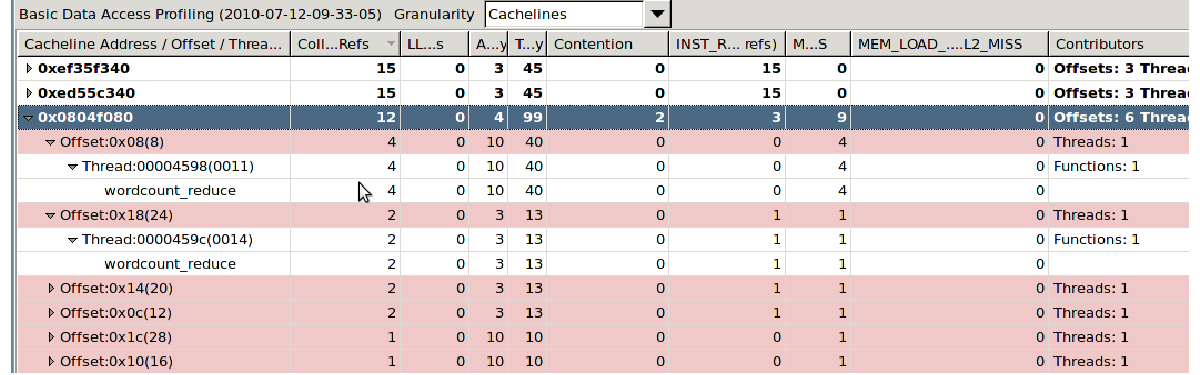
\includegraphics[width=6in]{sheriff/figure/wordcount}
\caption{PTU output for \texttt{word\_count}.
\label{fig:wordcount}}
\end{figure*}

\subsection{Detection Performance Overhead}
\label{sec:results-runtime-overhead}

\begin{figure*}[!t]
\centering
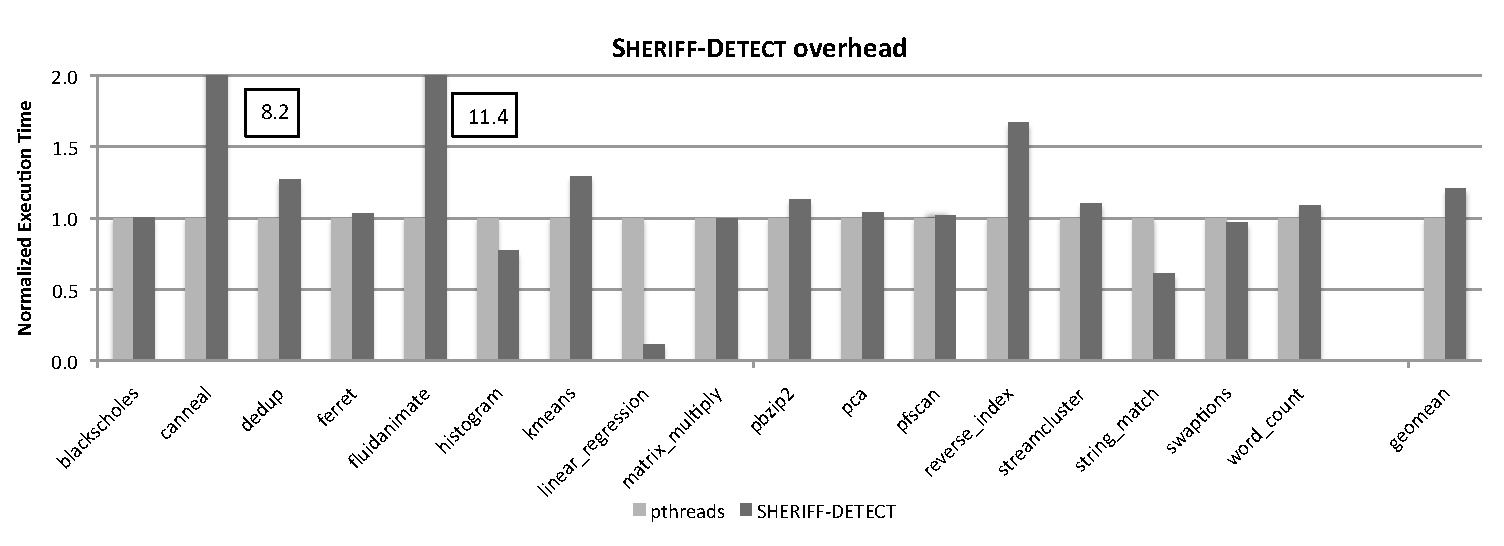
\includegraphics[width=6in]{sheriff/figure/detectiveperf.pdf}
\caption{\sheriffdetect{} performance overhead across two suites of benchmarks, normalized to the runtime of using the \pthreads{} library (lower is better). \label{fig:overhead}}
\end{figure*}


\SheriffDetect{}'s  runtime overhead (comparing to \pthreads{}) on two multithreaded benchmarks suites, Phoenix and PARSEC, is shown in Figure~\ref{fig:overhead}.  \SheriffDetect{} only introduces 20\% performance on average, with the exception of three outliers. For other benchmarks, \SheriffDetect{}’s overhead is generally acceptable and far lower than most existing tools.


\sheriffdetect{} do not perform well on two benchmarks. \texttt{canneal} runs about $7\times$ slower than that with \pthreads{}.  \texttt{fluidanimate}'s  performance overhead is about $11\times$ slower than that using \pthreads{}.

The first reason is that both benchmarks
trigger a high number of dirtied pages (3.4 million and
2.15 million, respectively). For each dirty page, \sheriffdetect{} applies page protection twice, creates a ``copy-on-write'' page and a ``twin'' page, checks false sharing problems at every sampling interval, and commits those local changes to the shared mapping. Thus, given large amount of dirty pages, copying overhead alone is very expensive and can dominate most of overhead. For example, \texttt{Canneal} invokes around 3.4 million dirty pages, thus leading to substantial overhead. 

Another reason for \texttt{fluidanimate} is that it invokes an unusually high number of transactions (16.7 million).  \SheriffDetect{} introduces page protection and commits overhead at every transaction boundary, thus, adding overhead if there are dirty pages.
 
 
However, even with these outliers that run slowly, the overhead of \SheriffDetect{} is generally acceptable
and far lower than most existing tools. \SheriffDetect{} actually improves performance by eliminating false sharing, using its process-as-threads framework. \SheriffProtect{} further reduces overhead as the next section describes.

\texttt{linear\_regression} runs $8\times$ faster with \SheriffDetect{} than with \pthreads{}, even with the added overhead of protection, memory commits, sampling and 
other mechanisms.  There is a serious false sharing problem inside (see Table~\ref{table:perfafterfix},) which both \sheriffdetect{} and \sheriffprotect{} eliminate automatically. Other cases where \sheriffdetect{}
outperforms \pthreads{} are also due to false sharing elimination. 


%%%%%%%%%%%%%%%%%%%%%%%%%%%%%%%%%%%%%%%5
%%%% Some data to list the effectiveness of this tool.
%%%%%% How many caches are carried for each test case. 
%%%%%% Whether all caches has false sharing problem.
%%%%%%%%%%%%%%%%%%%%%%%%%%%%%%%%%%%%%%%
\subsection{Detection Sampling Rate Sensitivity}
\label{sec:results-sampling-overhead}

\SheriffDetect{} employs the sampling mechanism to detect false sharing happening in long-running transactions. Sampling is only triggered when the length of a transaction exceeds a pre-defined threshold, usually 10ms. By handling those \texttt{SIGALARM} signals, \SheriffDetect{} tracks memory accesses by by comparing the temporary twin page against its
corresponding working version, and updates status words of specific cache lines. Thus, increased sampling rates may uncover more false sharing problems, but at the cost of increase performance overhead. 

To measure \sheriffdetect{}'s sensitivity to different sampling rates, we evaluate on three different sampling rates: 2ms, 10ms (our baseline), and 50ms.

\paragraph{Sampling Overhead:} Figure~\ref{fig:sensitivity} shows the performance overhead under different sampling rates, normalized to the runtime of using the default 10ms sample rate. For most of these benchmarks, sampling imposes relatively little overhead either because the average
number of shared pages is small, or because the
transaction length is often shorter than the sampling interval (thus no adding checking overhead).

One outlier is \texttt{canneal}, which is extremely sensitive to a different sampling rate.  When the sampling rate is 2ms, \texttt{canneal} runs about $2.3\times$ slower than that with  a 10ms sampling rate; \texttt{canneal} runs 35\% slower with a 50ms sampling rate than 2 10ms
sampling rate. The reason is that \texttt{canneal} dirties a large number of shared pages. More frequent sampling thus creates more temporary ``twin'' pages and increases checking overhead.


\begin{figure*}[!t]
\centering
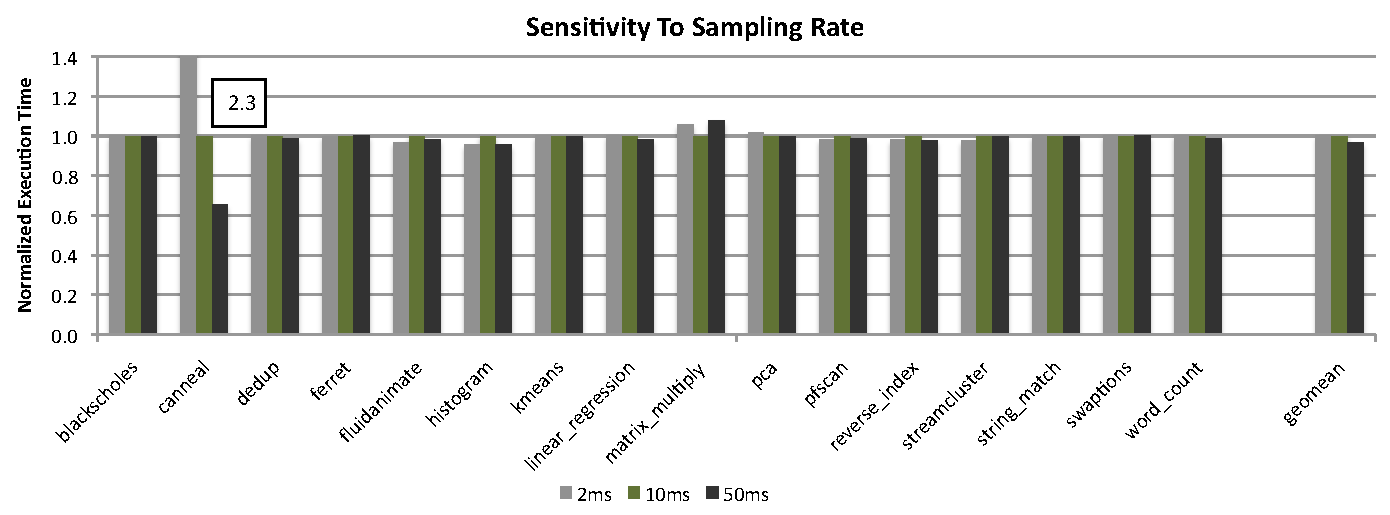
\includegraphics[width=6in]{sheriff/figure/sensitivity}
\caption{\sheriffdetect{} performance with different sampling rates,  normalized to the performance with a sampling interval of 10ms (presented in Figure~\ref{fig:overhead}); lower is better.
\label{fig:sensitivity}}
\end{figure*}

\begin{table*}[!t]
\centering
\resizebox{\columnwidth}{!}{
\begin{tabular}{l|rr|rr|rr}
\hline
{\bf \small Benchmark} & \multicolumn{2}{c|} {\bf \small 2ms} & \multicolumn{2}{c|} {\bf \small 10ms}& \multicolumn{2}{c} {\bf \small 50ms}\\
& {\em objs}  & {\em writes} & {\em objs}  & {\em writes} & {\em objs}  & {\em writes} \\
\hline
\small \texttt{canneal} & 1 & 21444321 & 1 & 26369324 & 1 & 30580451 \\
\small \texttt{ferret} & 1 & 3 & 0 & 0 & 0 & 0 \\
\small \texttt{fluidanimate} & 1 & 3370 & 1 & 4064 & 1 & 2851 \\
\small \texttt{kmeans} & 2 & 2974 & 2 & 1122 & 1 & 98 \\
\small \texttt{linear\_regression} & 1 & 1050 & 1 & 311 & 1 & 71 \\
\small \texttt{reverse\_index} & 5 & 14494 & 5 & 14782 & 5 & 14981 \\
\small \texttt{streamcluster} & 2 & 52462 & 1 & 52283 & 1 & 52420 \\
\small \texttt{word\_count} & 4 & 9849 & 4 & 2699 & 3 & 622 \\
\hline
\end{tabular}
}
\caption{
\sheriffdetect{} precision with different sampling rates, including the number of falsely-shared objects and interleaved writes. We omit those benchmarks with no observed cases of false sharing.
\label{table:samplingquality}}
\end{table*}

\paragraph{Sampling Effectiveness:}
The choice of sampling rates has relatively little impact on detection and ranking, shown in Table~\ref{table:samplingquality}. As expected, the number of falsely-shared objects reported and the number of interleaved writes observed are not significantly different.

Using a different sampling rate does affect the number of falsely-shared objects detected, but \SheriffDetect{} already reports all instances with a significant performance impact under the default sampling rate. Increasing the sampling rate to 2ms (more frequent sampling) reveals two additional falsely-shared objects (in \texttt{ferret} and \texttt{streamcluster}), but these two objects do not have a significant performance impact since they can only cause few cache invalidations(under 10). Similarly, reducing the sampling rate to 50ms (less frequent sampling) cannot detect two false sharing problems (in \texttt{kmeans} and \texttt{word\_count}), but these objects also have little impact on performance.


\subsection{Prevention Effectiveness}
\label{sec:protectperformance}

\begin{figure*}[!t]
\centering
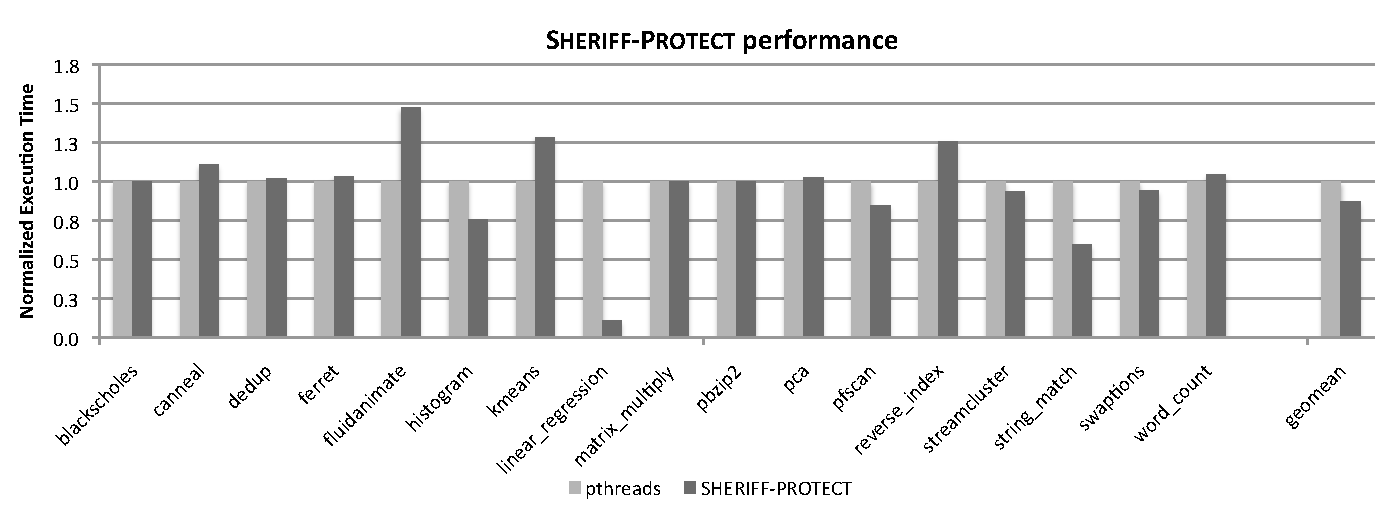
\includegraphics[width=6in]{sheriff/figure/patrolperf.pdf}
\caption{\sheriffprotect{} performance across two suites of benchmarks, normalized to the performance of \pthreads{} (see Section~\ref{sec:results-runtime-overhead}). In case of catastrophic false sharing, \sheriffdetect{} dramatically increases performance.
\label{fig:patrol}}
\end{figure*}

\begin{table}[!t]
\centering
\begin{tabular}{l|r|r}
\hline
{\bf \small Benchmark} & \multicolumn{2}{c} {\bf \small Normalized Runtime} \\
% \cline{2-3}
 & {\bf \small \sheriffdetect{} }  & {\bf \small \sheriffprotect{}} \\
\hline
\small \texttt{blackscholes} & 1.00 & 1.00 \\
\small \texttt{canneal} &  8.23 & 1.11 \\
\small \texttt{dedup} & 1.27 & 1.02 \\
\small \texttt{ferret} & 1.03 & 1.03\\
\small \texttt{fluidanimate} & 11.39 & 1.47 \\
\small \texttt{histogram} & \textbf{0.77} & \textbf{0.76} \\\small \texttt{kmeans} & 1.29 & 1.28 \\
\small \texttt{linear\_regression} & \textbf{0.12} & \textbf{0.11} \\
\small \texttt{matrix\_multiply} & 1.00 & 1.00 \\
\small \texttt{pbzip2} & 1.13 & 1.00 \\
\small \texttt{pca} & 1.04 & 1.03 \\
\small \texttt{pfscan} & 1.02 & \textbf{0.85} \\
\small \texttt{reverse\_index} & 1.67 & 1.25 \\
\small \texttt{streamcluster} & 1.10 &  \textbf{0.94} \\
\small \texttt{string\_match} & \textbf{0.61} & \textbf{0.60} \\
\small \texttt{swaptions} & \textbf{0.97} & \textbf{0.94} \\
\small \texttt{word\_count} & 1.09 & 1.05\\
\hline
\small \textbf{\em Geomean} & 1.21 & \textbf{0.87} \\
\hline
\end{tabular}
\caption{Detailed execution times with \sheriffdetect{} and \sheriffprotect{}, normalized to execution with the \pthreads{} library; numbers below 1 (boldfaced) indicate a speedup over \pthreads{}.
\label{table:detailedperf}}
\end{table}

We also examine the effectiveness of eliminating false sharing problems of using \SheriffProtect{}.  Figure~\ref{fig:patrol} presents the performance under \SheriffProtect{} and \pthreads{}.  For most cases, \SheriffProtect{} either has no effect on performance (when there is no false sharing problem inside) or improves the performance. Table~\ref{table:detailedperf} presents detailed performance results of \SheriffDetect{} and \SheriffProtect{}. 

\SheriffProtect{} improves the performance when an application is detected to have false sharing problems inside.  \texttt{linear\_regression} exhibits almost a $10\times$ speedup against the one using \pthreads{}, by tolerating a serious false sharing problem inside (see Table~\ref{table:perfafterfix}). \texttt{histogram} runs substantially faster with \SheriffProtect{} (24\%) because of preventing a read-write false sharing problem, see Section~\ref{sec:predatoreffective}. \texttt{string\_match} runs 40\% faster because of its custom memory allocator, preventing two threads allocating different objects from the same cache line, which is why \SheriffDetect{} does not find. 

Using \SheriffProtect{}, three benchmarks runs up to 47\% slower than using \pthreads{} because of different reasons. 
\texttt{kmeans} creates more than 3000 threads in eight seconds. Since the overhead of creating one process is higher than that of creating one thread, this dominates most of its overhead. For \texttt{reverse\_index} and \texttt{fluidanimate}, they exhibit slowdown because of using the processes-as-threads framework: Operating on those file-based pages is more expensive than operating on anonymous pages (the normal status of heap pages) under the Linux operating system; Writing to one page (\texttt{MAP\_SHARED}) cause a Copy-On-Write operation in the kernel even when there is only one user.  

Because \texttt{fluidanimate} has an enormous number of transactions(18 Million), \sheriffprotect{} 
introduces some additional overhead for every transaction. That also accounts for part of overhead.



\chapter{\Predator{}: Predictive False Sharing Detection}
\label{chapter:preditor}

This chapter presents \Predator{}, which improves the effectiveness of false sharing detection. \SheriffDetect{} reports false sharing accurately and precisely with only $20\%$ performance overhead. However, it can only detect the write-write type of false sharing for those programs using \pthreads{}. \SheriffDetect{} can also break programs that communicate across different threads using stack variables or self-defined synchronizations. These shortcomings greatly limit \SheriffDetect{}'s usage on real-world applications.  

In contrast to \SheriffDetect{}, \Predator{} detects all types of false sharing and has no limitations on applications. \Predator{} has been utilized to find actual false sharing problems of real applications, including \texttt{MySQL} and the \texttt{Boost} library.

In addition, \SheriffDetect{} and other systems share one key limitation: they can only report \emph{observed} cases of false sharing. As Nanavati et al.\ point out, false sharing is sensitive to where objects are placed in cache lines and so can be affected by a wide range of factors~\cite{OSdetection}. For example, using the gcc compiler \emph{accidentally} eliminates false sharing of the linear\_regression benchmark at certain optimization levels, while LLVM does not do so at any optimization level.  A slightly different memory allocation sequence (or different memory allocator) can reveal or hide false sharing, depending on where objects end up in memory; using a different hardware platform with different addressing or cache line sizes can have the same effect. All of this means that existing tools cannot root out potentially devastating cases of false sharing that could arise with different inputs, in different execution environments, and on different hardware platforms.

\Predator{} is the first system that can \emph{predict} potential false sharing that does not manifest in an execution, but may appear and greatly degrade the performance of programs in a slightly different environment. Predictive false sharing generalizes from a single execution to identify potential false sharing instances that fall into two adjacent cache lines, which could be exposed by slight changes in object placement and alignment. It also can predict false sharing in hardware platforms with larger cache line sizes by tracking accesses within \emph{virtual cache lines} that span multiple physical lines. Predictive false sharing detection thus help avoids the predicament of previous detection tools: those problems can easily leak to deployment environment because of the changed execution environment.

Here, we first describe \Predator{}'s false sharing detection mechanism in Section~\ref{sec:detection}, which consists of both compiler and runtime system components. Section~\ref{sec:prediction} then explains how \Predator{} predicts potential false sharing based on a single execution.

\section{False Sharing Detection}
\label{sec:detection}

\subsection{Overview}
\label{sec:overview}
\Predator{} follows the same idea of detecting false sharing, described in Section~\ref{sec:detectionidea}. We compute cache invalidations based only on memory accesses history of each cache line, and only report those instances that may affect performance. 

\Predator{} is based on the similar {\it basic observation}: if a thread writes a cache line after other threads have accessed the same cache line, this write operation causes at least a cache invalidation. Drawing from this observation, \Predator{} tracks cache invalidations of all cache lines and ranks the severity of performance degradation  according to the number of cache invalidations. 
% by keeping track of accesses from different threads. 
 
To track memory accesses, \Predator{} relies on the compiler instrumentation. The design tradeoff of choosing compiler instrumentation, instead of other mechanisms, has been discussed in Section~\ref{sec:instrumentationtradeoff}. A compiler can easily identify read or write accesses. However, a compiler does not know how and when those instructions are being executed, since that depends on a specific execution, input, and runtime environment.

Therefore, \Predator{} combines a runtime system with compiler instrumentation to track cache invalidations: the compiler instruments memory accesses so the runtime system is notified when an access is executed (see Section~\ref{sec:compiler}), and the runtime system is responsible for collecting and analyzing actual memory accesses to detect and report false sharing (see Section~\ref{sec:runtime}).

\subsection{Compiler Instrumentation}
\label{sec:compiler}

\Predator{} relies on LLVM to perform instrumentation at the intermediate representation level~\cite{llvm}.
It traverses all functions one by one and searches for memory accesses to those global and heap variables.  For each memory access, \Predator{} instruments a function call to invoke the runtime system, passing with the address, access type and unit of this memory access (how many bytes). \Predator{} currently omits accesses to stack variables by default because stack variables are normally used for thread local storage and therefore do not normally introduce false sharing. However, instrumentation on stack variables
can always be turned on when necessary.

The instrumentation pass is placed at the very end of the LLVM optimization passes so that only those memory accesses surviving all previous LLVM optimization passes are instrumented.  This technique is similar to the one used by AddressSanitizer~\cite{AddressSanitizer}.

\subsection{Runtime System}
\label{sec:runtime}

\Predator{}'s runtime system collects every memory access by handling those functions calls inserted during the compiler instrumentation phase. It analyzes possible cache invalidations based on the basic observation discussed in Section~\ref{sec:overview}. Finally, it precisely reports any performance-degrading false sharing problems it finds.  For global variables involved in false sharing, \Predator{} reports their name, address and size; for heap
objects, \Predator{} reports the callsite stack for their allocations, address and size. In addition, \Predator{} provides word granularity access information for those cache lines involved in false sharing: how many reads or writes are issued by which thread.  This information can further help users diagnose and fix false sharing instances.

\subsubsection{Tracking Cache Invalidations}
\Predator{} only reports those global variables or heap objects on cache lines with a large number of cache invalidations, thus possibly affecting performance of applications. To track cache invalidations, \Predator{} maintains a two-entries-cache-history table for each cache line.  In this table, each entry has two fields: thread ID and access type (read or write). Thread ID is used to identify the origin of each access. As stated earlier, only accesses from different threads (with a different thread ID) can cause a cache invalidation.

For every new access to a cache line $L$, \Predator{} checks $L$'s history table $T$ to decide whether the current access leads to a cache invalidation.  As described in Section~\ref{}, only write accesses can cause cache invalidations and read accesses only create a copy of data in the cache of the current core that the current thread is running on. Also, it is noticed that table $T$ only has two status: full and not full.  There is no ``empty'' status since every cache invalidation should replace its table with the current write access, setting the first entry to the current access (with its thread ID and write access type).

\begin{itemize}
\item
  For a read access $R$, 
  \begin{itemize}
    \item
      If $T$ is full, there is no need to record this read access.
    \item
      If $T$ is not full and another existing entry has a different thread
      ID, then \Predator{} records this $R$ (and its thread) by adding a new entry to the table. 
  \end{itemize}
\item
  For a write access $W$, 
  \begin{itemize}
    \item
      If $T$ is full, then $W$ can cause a cache invalidation since at least one of two existing accesses are issued by a different thread (one thread can only occupy one entry).
      After recording this invalidation, \Predator{} updates the existing entry with $W$(and its thread).
    \item
      If $T$ is not full,
      \Predator{} checks whether $W$ and the existing entry has the same thread ID. If so, $W$ cannot cause a cache invalidation and there is no need to do anything. Otherwise, \Predator{} identifies a possible cache invalidation on this line: it increments the number of cache invalidations and updates the existing entry with the current $W$ access.
  \end{itemize}
\end{itemize}

\subsubsection{Reporting False Sharing}
\label{sec:predatorcallsite}

\Predator{} reports false sharing precisely and accurately. Accurately means \Predator{} only reports those false sharing instances with a large number of cache invalidations, which may possibly cause performance problems. \Predator{} also differentiate actual false sharing from true sharing, since true sharing can also induce a large number of cache invalidations.

\Predator{} employs the following mechanisms to achieve this target, as well as reducing the performance overhead.  

\begin{itemize}
\item

In order to accurately differentiate those false sharing problems with true sharing problems, \Predator{} tracks word-level accesses for those cache lines involved in a big number of cache invalidations, which has been discussed in Section~\ref{sec:accuratedetect}.


\item
\predator{} relies on \texttt{backtrace()} function in the \texttt{glibc} library to obtain the whole callsite stack, which is slower but much more robust to be used than the ways used in \SheriffDetect{}. Thus, it can report the callsite stack for those heap objects. 


\item
For every access, \Predator{} needs to lookup the corresponding cache line's metadata. Because this operation is so frequent, at every access, lookups need to be very efficient. Like AddressSanitizer~\cite{AddressSanitizer} and other systems~\cite{Valgrind, qinzhao}, \Predator{} uses a shadow memory mechanism to store metadata for every piece of application data.  Thus, \Predator{} can compute and locate corresponding metadata directly via address arithmetic.

\item
In order to support shadow memory, \Predator{} uses a pre-defined starting address and fixed size for its heap.  It also contains a custom memory allocator, which is described in Section~\ref{sec:customheap}.  However, using this custom memory allocator also implies that false sharing caused by a memory allocator cannot be detected by \Predator{}: two threads allocate heap objects from the same cache line concurrently. But this should not be a serious problem since  all modern memory allocators, like Hoard, already avoid this kind of false sharing and we should always use this kind of memory allocator.

\end{itemize} 
 
\subsection{Optimizations}
\label{optimization}
Tracking every memory access can be extremely expensive, thus \Predator{} utilizes the following mechanisms to further reduce performance and memory overhead.

\subsubsection{Threshold-Based Tracking Mechanism}
\label{sec:thresholdtracking}
\Predator{} aims to detect false sharing that significantly degrades performance. Since cache invalidations are the root cause of performance degradation and only writes 
can possibly cause cache invalidations, 
cache lines with a small number of writes are never be a target with a significant performance impact.
For this reason, \Predator{} only tracks cache invalidations
once the number of writes to a cache line crosses a
pre-defined threshold, which we refer to as the {\it Tracking-Threshold}. 
Before this threshold is reached, \Predator{} only tracks the number of writes on a cache line while skipping tracking reads. This mechanism reduces performance and memory overhead
at the same time.

In the current implementation, \Predator{} maintains two arrays in shadow memory: 
{\it CacheWrites} tracks the number of memory writes on every cache line, and
{\it CacheTracking} tracks detailed information 
for each cache line once the number of writes on a cache line exceeds the {\it Tracking-Threshold}. 
If the threshold is not reached, there is no need to check the corresponding {\it CacheTracking}. 
Figure~\ref{fig:algorithm} illustrates the detailed mechanism.

\begin{figure}[!t]
\begin{lstlisting}[style=tt]
void HandleAccess(unsigned long addr, bool isWrite) {
 unsigned long cacheIndex=addr>>CACHELINE_SIZE_SHIFTS;
 cachetrack *track=NULL;

 if(CacheWrites[cacheIndex]<TRACKING_THRESHOLD) {
  if(isWrite) {
   if(ATOMIC_INCR(&CacheWrites[cacheIndex]) 
      ==TRACKING_THRESHOLD-1) {
     track=allocCacheTrack();
     ATOMIC_CAS(&CacheTracking[cacheIndex],0,track));
   }
  } 
 }
 else {
  track=CacheTracking[index]);
  if(track){
    // Track cache invalidations and detailed accesses
    track->handleAccess(addr, isWrite);
  }
 }
}
\end{lstlisting}
\caption{Pseudo-code of handling an access in \Predator{}.\label{fig:algorithm}}
\end{figure}

To avoid expensive lock operations, \Predator{} uses atomic instruction to increment the {\it CacheWrites} counter for each cache line. 
When the number of writes of a cache line reaches the predefined threshold,
it allocates space to track detailed cache invalidations and word-level information. \Predator{} also 
uses an atomic compare-and-swap to set the cache tracking address for this cache line in the shadow mapping.
After {\it CacheWrites} on a cache line reaches the {\it Tracking-Threshold}, all read and write accesses on this cache line are tracked.


\subsubsection{Selective Compiler Instrumentation}
\label{sec:selectinstrumentation}

\Predator{} relies on compiler instrumentation to provide memory access information to the runtime system 
and detects false sharing based on the sequences of memory accesses on every cache line. 
The performance overhead of a specific program is always proportional to the degree of instrumentation: more instrumentation generally indicates more performance overhead. 
Thus, \Predator{} provides a flexible framework to instrument programs depending on the performance requirements of the user.

Currently, \Predator{} only instruments once for each type of memory access on each address 
to the same basic block. 
This selective instrumentation does not normally affect the effectiveness of detection. 
Because \Predator{} aims to detect false sharing cases with a large number of cache invalidations,
less tracking of accesses inside a basic block can induce fewer cache invalidations, but it should not affect the overall behavior of cache invalidations. 

% detection will not cause performance problem. 
To improve performance further,
\Predator{} can be easily extended to support more flexible instrumentation as follows:
\begin{itemize}
\item
\Predator{} could selectively instrument both reads and writes or only writes.
Instrumenting only writes reduces overhead while detecting write-write false sharing, 
as \Sheriff{} does. 
\item
\Predator{} can be set to instrument or skip specific code or data. 
For example, the user could provide a black-list so that given modules,
functions or variables are not instrumented. 
Conversely, the user could provide a white-list so that only specified functions or variables are instrumented. 
\end{itemize}

\subsubsection{Sampling Mechanism}
\label{sec:sample}
As described in Section~\ref{sec:thresholdtracking}, when the number of writes on a cache line is larger than {\it Tracking-Threshold}, every
access must be tracked in detail: we have to track word-level 
information, update the number of accesses and possible cache invalidations, and update the cache access history table
of this cache line.  When a cache line is involved in false or true sharing, updating those counters can exacerbate the performance impact of sharing: not only is there an cache invalidation on this application's cache line, but there is also at least another cache invalidation caused by updating the metadata of this corresponding cache line.

To further reduce the performance overhead, \Predator{} only samples the first specified number of accesses during each sampling interval. 
Currently, \Predator{} maintains an access counter for each cache line
and only tracks the first $10,000$ accesses out of every 1 million accesses on a cache line, with 1\% sampling rate. Section~\ref{sec:predatorsensitivity} further evaluates the effect of different sampling rates on performance and effectiveness.  



\section{False Sharing Prediction}
% Why prediction is important?
\label{sec:prediction}
This section further motivates predictive false sharing and explains how to support it in the runtime system.  

\subsection{Overview}
%\begin{figure*}[!htb]
\label{sec:predictoverview}

\begin{figure}[!t]
\begin{center}
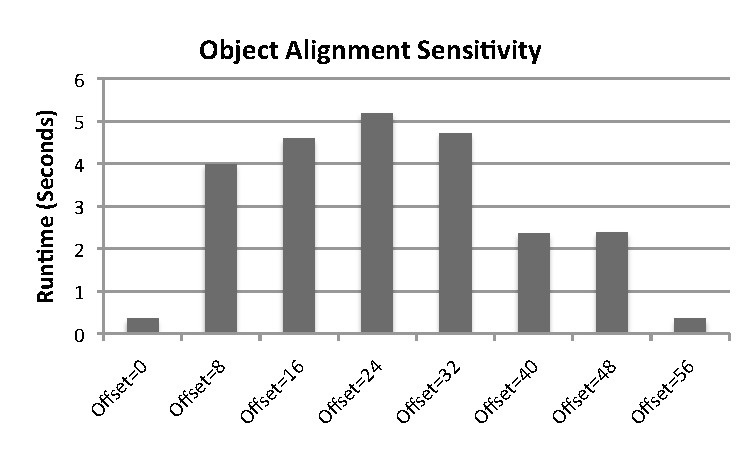
\includegraphics[width=6in]{predator/figure/perfsensitive}
\end{center}
\caption{
Performance of the linear\_regression benchmark (from Phoenix)  is highly sensitive to the memory layout between the (potentially) falsely-shared object and corresponding cache lines. 
\label{fig:perfsensitive}}
\end{figure}

The appearance of false sharing depends on 
the memory layout between objects and corresponding cache lines. The performance of a real example, linear\_regression, is shown in Figure~\ref{fig:perfsensitive}: 
When the offset of the starting address between the potentially falsely-shared object and corresponding cache lines is $0$ or $56$ bytes, there is no false sharing; 
When the offset is $24$ bytes, we see the most severe performance effect caused by false sharing. 
The performance difference caused by false sharing can affect the performance as large as $15\times$ on an 8-core machine. 

Existing detection tools can only report observed false sharing. That means, they may miss such a very severe false sharing problem that could occur in the wild if the offset of the starting address was $0$ bytes or $56$ bytes in their test environment. \Predator{} overcomes this shortcoming by accurately predicting potential false sharing, without the need of occurrences. 

\begin{figure*}
\begin{center} 
\subfigure[No false sharing]{%
   \label{fig:nofs}
   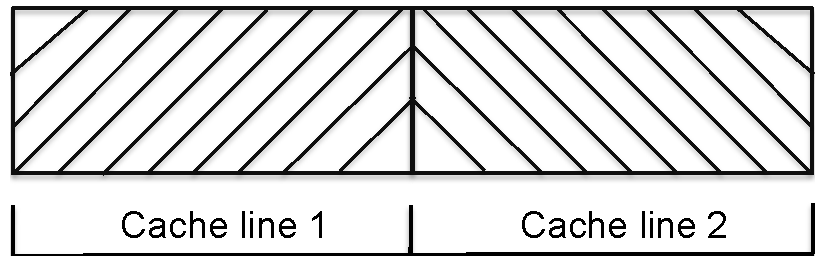
\includegraphics[width=0.24\textwidth]{predator/figure/Potential1}
}%
\hspace{10pt}
\subfigure[False sharing with larger cache size]{%
   \label{fig:fslarger}
   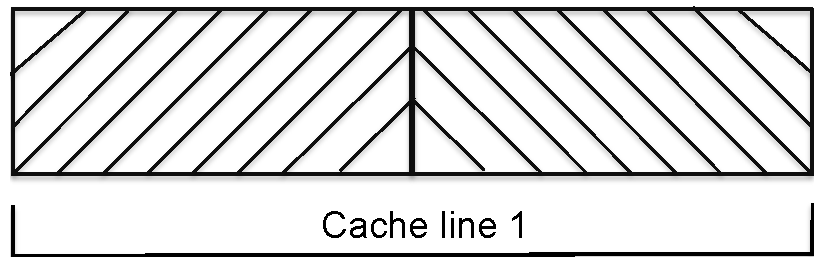
\includegraphics[width=0.24\textwidth]{predator/figure/Potential2}
}%
\hspace{10pt}
\subfigure[False sharing with different memory layout]{%
   \label{fig:fsnoalignment}
   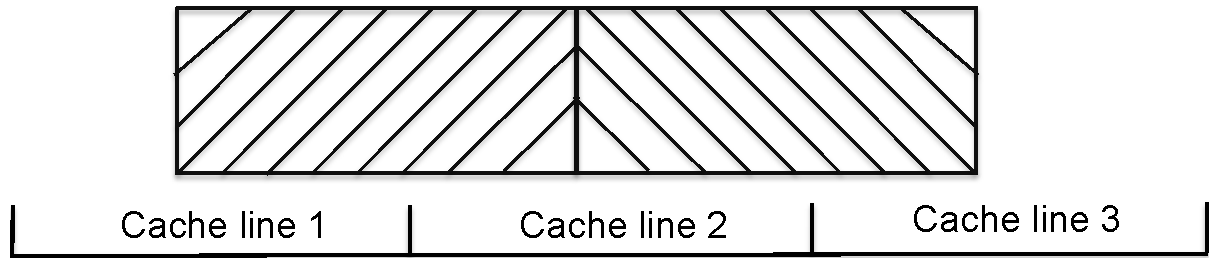
\includegraphics[width=0.36\textwidth]{predator/figure/Potential3}
}%
\end{center}
%\includegraphics{fig/potential.pdf}
\caption{False sharing under different environments.}
\label{fig:potentialfalsesharing}
\end{figure*}

\Predator{} predicts {\it potential false sharing}, which does not manifest in the current execution but may appear and greatly affect performance of programs in a slightly different environment.

Figure~\ref{fig:potentialfalsesharing} shows a simplified example why occurrences of false sharing can change in different situations. 
In this figure, two rectangles with different patterns
represents two portions of the same object, updated by different threads. In Figure~\ref{fig:nofs}, there is no false sharing when thread T1 only updates 
``cache line 1'' and T2 only updates ``cache line 2''.
However, false sharing appears in one of the following cases, even with the same
access pattern. 

\begin{itemize}
\item
Doubling cache line size (Figure~\ref{fig:fslarger}). When the size of a cache line doubles, both T1 and T2 access the same cache line concurrently, thus causing false sharing.

\item
Different starting address of an object(Figure~\ref{fig:fsnoalignment}).  
When the starting address of this object is not aligned with the starting address of the first cache line, then T1 and T2 can update the second cache line simultaneously, causing a false sharing problem. 
%When some dynamic property changes the starting address of this object so that it 
%is not aligned with the starting address of the first cache line, 
\end{itemize} 

\Predator{} predicts whether programs can have potential false sharing in one of these two situations, where they can be caused by different dynamic properties. These dynamic properties include choosing a different compiler, enabling different compiler optimizations, using a different memory allocator, adding or removing code involving in memory allocations, switching to a different target platform with a different address mode (32-bit or 64-bit), and changing the size of cache line (64 Bytes or 128 Bytes). 
All dynamic properties, except changing the size of cache line, can lead to a different memory layout, thus can possibly affect occurrences of a false sharing problem. Thus, predicting false sharing in changing the memory layout or changing the size of cache line actually explores many possibilities caused by all of these dynamic properties.

\subsection{Basic Prediction Workflow}
\label{sec:predictionmechanism} 

%Similar to the detection part, 
\Predator{} focuses on potential false sharing that can 
cause performance problems.
It is based on two key observations. First, only accesses to 
adjacent cache lines can lead to potential false sharing, 
i.e., introducing cache invalidations when the cache line size
or an object's starting address changes.
Second, only those cache lines with a large number of cache invalidations can degrade performance.

Based on these two observations, \Predator{} develops 
the following workflow to predict potential false sharing.
Those detection optimizations listed in Section~\ref{optimization} can also be applied
to here. We do not repeat these optimizations in this section.

\begin{enumerate}
\item
Track the number of writes on different cache lines. 

\item
When the number of writes to a cache line $L$ reaches {\it Tracking-Threshold},
\predator{} tracks the detailed read and write accesses for every word on both cache line $L$ 
and its adjacent cache lines. 

\item
When the number of writes to a cache line $L$ reaches a second threshold (called as
{\it Predicting-Threshold}), 
\predator{} identifies whether there exists false sharing in $L$ and its adjacent cache lines by analyzing word accesses information collected in Step 2, which are described in 
Section~\ref{sec:evaluatingfs} in detail.

\item
If a potential false sharing is found, \predator{} starts to track cache line invalidations in order to confirm its seriousness, which are discussed in Section~\ref{sec:tracking}.
Otherwise, go back to Step 2 to track more detailed accesses.
 
\end{enumerate}

\subsection{Searching for Potential False Sharing}
\label{sec:evaluatingfs}
To describe potential false sharing in two different cases, we first introduce a concept -- ``virtual cache line''.  A virtual cache line is a contiguous memory range that spans one or more physical cache lines.  

In the case of double cache line size, a virtual line is composed of two originally contiguous cache lines, where it starts with a even number cache line.  Thus, only cache lines $2*i$ and $2*i+1$ can form a virtual cache line.  

To evaluate a potential false sharing problem that can be caused by changing memory layout, a virtual line should have the same size as an actual cache line, but with a different starting address: unlike actual cache lines, the
starting address of a virtual cache line does not need to be multiple of the cache line size. For instance, a 64-byte-long virtual line can consist of the range $[0,64)$ bytes or $[8,72)$ bytes.

To search for a potential false sharing problem, 
\Predator{} searches for a pair of hot accesses, one on $L$ and one on its previous or next cache line, based on detailed word information collected in Step 2. Two accesses happening in the same actual cache line should be detected by the normal detection mechanism, thus they can lead to actual false sharing problems but not a potential false sharing problem. 

A hot access refers to an access that has the number of read or write accesses larger than the average number of accesses. In fact, for every hot access $X$ in a specific cache line $L$, \Predator{} searches another
hot access $Y$ in $L$'s previous cache line or next cache line, satisfying the following conditions: 

\begin{itemize}
\item
$X$ and $Y$ reside on the same virtual line. 

\item
One of $X$ and $Y$ is a write access.

\item 
$X$ and $Y$ are issued by different threads.

\end{itemize}

% why it finds a pair of $X$ and $Y$ == a potential false sharing 
Whenever it finds such a pair, $X$ and $Y$, 
\Predator{} identifies a potential false sharing problem: they can degrade performance when the number of cache invalidations possibly caused by $X$ and $Y$ (on a possible virtual line), is larger than a pre-defined threshold. This approach is based on a similar observation as in detection: \emph{if a thread writes a virtual line after other threads have accessed the same virtual line, this write operation causes at least one cache invalidation}. 

However, before tracking detailed memory accesses on a specific virtual line, it is impossible to know exactly how many cache invalidations actually happen on this virtual line. Thus, \Predator{} conservatively assumes that accesses from different threads occurs in a interleaved way, with the maximum number of cache invalidations. Then \Predator{} starts to track possible cache invalidations on a virtual covering both $X$ and $Y$, described in Section~\ref{sec:tracking}.  

%According to above observation and assumption, 
%a pair of hot accesses, $X$ and $Y$, if accesses are issued in an interleaving 
%way, can generate the number of cache invalidations equaling to 
%the smaller number of accesses of $X$ and $Y$.
%Thus a false sharing problem is to be identified by \Predator{}.
  

\subsection{Verifying Potential False Sharing}
\label{sec:tracking}

\Predator{} verifies potential false sharing by tracking possible cache invalidations on a specific virtual line covering such a hot access pair, $X$ and $Y$.
%covering a pair of hot accesses found
%in Step 3.

For potential false sharing caused by double cache line size, as described in Section~\ref{sec:evaluatingfs}, a virtual line is always composed of cache line with index $2*i$ and $2*i+1$. 
\Predator{} tracks cache invalidations on a virtual line that covering $X$ and $Y$. This virtual line is unique for a given $X$ and $Y$ pair. 

However, for the case of changing memory layout, two hot accesses with distance less than the cache line size 
can actually form multiple virtual lines. 
There is thus an additional step to determine which virtual line to be tracked. 
Although a virtual line to be chosen here is never a real cache line of actual hardware because of unaligned addresses,
we utilize this virtual line to simulate the effect of changing memory layout correspondingly.


\begin{figure}
\begin{center} 
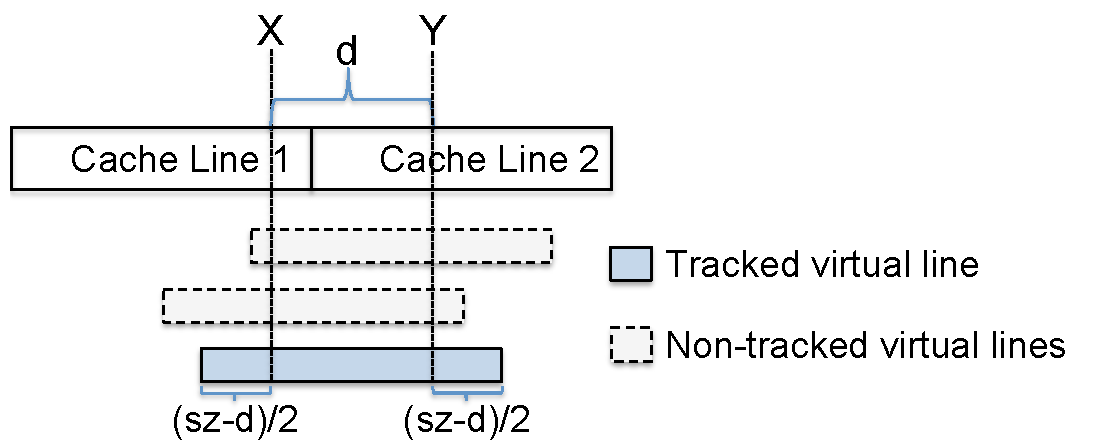
\includegraphics[width=6in]{predator/figure/trackpotential}
\end{center}
\caption{Determining a virtual line with size $sz$ according to hot accesses.}
\label{fig:trackpotential}
\end{figure}

Figure~\ref{fig:trackpotential} shows that multiple virtual lines can cover $X$ and $Y$. However, \Predator{} only chooses one of these virtual lines. \Predator{} chooses the virtual line that leaves the same space before $X$ and after $Y$. That is, the virtual line starting at location $X-((sz-d)/2)$ and ending at $Y+((sz-d)/2)$ is tracked by \Predator{}. This choice allows tracking of more possible cache invalidations caused by adjacent accesses of $X$ and $Y$. Since adjusting the starting address of a virtual line has the same effect of adjusting the starting address of an object in detecting false sharing, all cache lines related to the same object must be adjusted at the same time. \Predator{} then tracks cache invalidations based on these adjusted virtual lines.

In the end, \Predator{} can report accurately whether the change of memory layout can affect the performance or not, based on the possible number of cache invalidations. 

Currently, \predator{} only determines a specific virtual line to be tracked. However, we plan to extend this in the future work by using a much more flexible mechanism: we can choose a different virtual line after a number of accesses if the current choose cannot reveal a big number of cache invalidations.



\section{Evaluation}



\label{sec:evaluation}

This section answers the following questions:
\begin{itemize}
\item
  How effective is \Predator{} at detecting and predicting false sharing?

\item
  What is \Predator{}'s overhead, in terms of execution time and memory ?

\item
  How sensitive is \Predator{} to different sampling rates?
 
\end{itemize}

\paragraph{Experimental Platform.} All evaluations are performed on a quiescent Intel Core 2 dual-processor system,  equipped with 16GB RAM in total. Each processor is a 4-core 64-bit Intel Xeon running at 2.33 GHz, with a 4MB shared L2 cache and 32KB private L1 cache. The underlying operating system is an unmodified CentOS 5.5, running with Linux kernel version 2.6.18-194.17.1.el5. The glibc version is 2.5. 

\paragraph{Evaluated Applications.}
This paper evaluates two popular benchmark suites,
Phoenix (with large input) ~\cite{phoenix-hpca} and PARSEC (with simlarge input) ~\cite{parsec}. Even with unmodified LLVM-3.2, Facesim cannot be compiled successfully (having complaints on an undefined template) and Canneal aborts unexpectedly. Thus, these two benchmarks are excluded.
We also evaluate \Predator{} on six real applications, including MySQL, Boost, Memcached, aget, pbzip2 and pfscan.



\subsection{Detection and Prediction Effectiveness}
\label{sec:predatoreffective}

\begin{figure*}[htb]
{\centering
\tiny
\subfigure{\lstinputlisting[numbers=none,frame=none,boxpos=t]{predator/figure/linearregression.report}}
\caption{An example reported by \Predator{}, indicating a potential false sharing problem in the linear\_regression benchmark.
\label{fig:lrreport}}
}
\end{figure*}

For every false sharing problem, \Predator{} reports source code information and detailed memory access information in order to help users fix those problems. Figure~\ref{fig:lrreport} shows an example for the linear\_regression benchmark. This report shows that the heap object starting with $0x40000038$ potentially causes a large number of cache invalidations. The call stack of this memory allocation is provided to help locate culprits. In addition, \Predator{} also reports word-level access information of this object, which helps to identify where and how false sharing occurs. From that, we can know that it is a latent false sharing problem predicted by \Predator{}, since different threads are accessing different cache lines. 

\subsubsection{Benchmarks}
\label{sec:benchmarks}

\begin{table}[!t]
{\centering
\resizebox{\columnwidth}{!}{
\begin{tabular}{l|r|r|r|r|r}\hline
{\bf \small Benchmark} & {\bf \small Source Code} & {\bf \small New} & {\bf \small Without Prediction} &{\bf \small With Prediction} & {\bf \small Improvement} \\
\hline
\small \textbf{histogram} & {\small histogram-pthread.c:213} & \cmark{} &\cmark{} & \cmark{} & 46.22\%\\
\small \textbf{linear\_regression} & {\small linear\_regression-pthread.c:133} & & & \cmark{} & 1206.93\% \\
\small \textbf{reverse\_index} & {\small reverseindex-pthread.c:511} & & \cmark{} & \cmark{} & 0.09\%\\
\small \textbf{word\_count} & {\small word\_count-pthread.c:136} & & \cmark{} & \cmark{} & 0.14\%\\
\hline
\small \textbf{streamcluster} & {\small streamcluster.cpp:985} &  & \cmark{} & \cmark{} &7.52\% \\
\small \textbf{streamcluster} & {\small streamcluster.cpp:1907} & \cmark{} & \cmark{} & \cmark{} & 4.77\%\\
\hline
\end{tabular} }
\caption{False sharing problems in the Phoenix and PARSEC benchmark suites. \label{table:detection}}
}
\end{table}

We evaluate \Predator{}'s effectiveness on two benchmark suites, Phoenix and PARSEC, and Table~\ref{table:detection} presents those benchmarks with false sharing problems. 
The first column lists those programs with false sharing problems.  The second column shows precisely where the problem is. Because all discovered false sharing occurs inside heap objects, we show the source code information of callsite here.  The third column, ``New'', marks whether this false sharing was newly discovered by \Predator{}.  A checkmark in the  following two columns indicates whether the false sharing was identified without prediction or with prediction enabled.  The final column, ``Improvement'', shows the performance improvement after fixing false sharing. Note that the performance improvement shown here is different with that in Table~\ref{table:perfafterfix} because \SheriffDetect{} evaluates on a 32bit platform and \Predator{} evaluates on a 64bit platform. This also shows that performance effect is every sensitive to hardware platform, which is one of dynamic properties that we discussed above. 
%The number is based on the average runtime of $10$ runs. 

As shown in the table, \Predator{} reveals two unknown false sharing problems. It is the first tool to uncover false sharing in histogram and at line $1907$ of streamcluster. 
In histogram, multiple threads simultaneously modify different locations of the same heap object, thread\_arg\_t. 
Padding this data structure fixes the false sharing problem and improves the performance by around 46\%. In streamcluster, multiple threads are simultaneously accessing and updating the same \texttt{bool} array, switch\_membership. Simply changing all elements of this array to a long type reduces the false sharing effect, improving performance by about 4.7\%.

%, although it is not a complete fix of false sharing. 
%None of these two false sharing problems has been reported by previous tools.
Other false sharing problems were discovered by previous work~\cite{sheriff}. The detailed reason of false sharing problems and how they are fixed are discussed in Section~\ref{sec:effecteval}.

It is worth noting that linear\_regression has a potential false sharing problem according to the execution environment of \Predator{}. According to the observation of Nanavati et al., this false sharing problem occurs when using clang and disappears when using gcc with the -O2 and -O3 optimization level~\cite{OSdetection}. But we observed a different result: when we are using the clang-3.2 compiler and our custom memory allocator, the false sharing problem does not occur at all because the offset happens to be 56 bytes (see Figure~\ref{fig:perfsensitive}). 
However, it does occur in the original execution environment, with the default memory allocator and using gcc compiler. That is why fixing it improves the performance by more than $12\times$.  This also exemplifies the necessity of \Predator{} predictive detection: existing tools may miss a false sharing problem if it does not occur at their test environments. 
 
\subsubsection{Real Applications}
To verify \Predator{}'s practicality, we further evaluate several widely-used real applications, whereas no previous work has done this. These real applications include a server application (MySQL~\cite{mysql}),
a standard C++ library (Boost~\cite{libfalsesharing}),
a distributed memory object caching system (Memcached), a network retriever (aget),
a parallel bzip2 file compressor (pbzip2), and a parallel file scanner (pfscan).

MySQL-5.5.32 and boost-1.49.0 are known to have false sharing problems. Other applications (memcached-1.4.15, aget-0.4.1,  pbzip2-1.1.6, and pfscan) do not have known false sharing problems.

The false sharing of MySQL has caused a significant scalability problem and was very difficult to be identified.
According to the architect of MySQL, Mikael Ronstrom, ``we had gathered specialists on InnoDB..., participants from MySQL support... and a number of generic specialists on 
computer performance...'', ``[we] were able to improve MySQL performance by 6$\times$ with those scalability fixes''~\cite{mysql}. 
The false sharing inside Boost is caused by the usage of a  spinlock pool. Different threads may utilize different spinlocks located in the same cache line in this case. Reducing the number of spinlocks on per cache line to 1 brings a 40\% performance improvement.
\Predator{} is able to pinpoint false sharing locations in both MySQL and the Boost library. 
For the other four applications, \Predator{} does not find severe false sharing problems.

\subsubsection{Prediction Effectiveness}
\label{sec:predicteval}
In this section, we verify whether prediction can always  reveal un-observed false sharing problems.

The linear\_regression benchmark is evaluated here because of the following two reasons: (1) The false sharing problem of this benchmark cannot be detected without prediction; (2) The false sharing problem severely degrades performance when it actually occurs, thus it is a serious problem that should be detected. 

\begin{figure}
\begin{lstlisting} [style=tt]
struct
{
  pthread_t tid;  POINT_T *points;
  int num_elems;  long long SX;
  long long SY;   long long SXX;
  long long SYY;  long long SXY;
} lreg_args;

void * lreg_thread ( void * args_in ) {
  struct lreg_args * args = args_in ;
  for(i=0; i<args->num_elems; i++) {
    args->SX+=args->points[i].x;
    args->SXX+=args->points[i].x*args->points[i].x;
    args->SY+=args->points[i].y;
    args->SYY+=args->points[i].y*args->points[i].y;
    args->SXY+=args->points[i].x*args->points[i].y;
  }
}
\end{lstlisting}
\caption{The false sharing problem inside the linear\_regression benchmark: multiple threads simultaneously update distinct entries of a global array.
\label{fig:linearregression}}
\end{figure}

Figure~\ref{fig:linearregression} shows the data structure and the code exercising corresponding false sharing. The size of this data structure, lreg\_args, is $64$ bytes 
when the program is compiled to a $64$-bit binary using llvm compiler, with optimization level ``-O3''. In this benchmark, the main thread allocates an array, containing as the same number of elements as hardware cores. Each element is a lreg\_args type with $64$ bytes. This array is then passed to different threads (lreg\_thread function) so that each thread only updates its thread-dependent area. False sharing occurs if two threads happen to update a cache line. 

Figure~\ref{fig:perfsensitive} shows how sensitive the performance is to different starting addresses of this falsely-shared object. When the offset is $0$ or $56$ bytes, this benchmark achieves its optimal performance and has no false sharing. When the offset is $24$ bytes, the benchmark runs about $15$ times slower than its optimal performance because of the false sharing problem.

Our evaluation shows that \Predator{} can always detect the false sharing problem with prediction enabled, when this false  sharing object starts with different offsets. This demonstrates the effectiveness of its prediction mechanism.

\subsection{Performance Overhead}
\label{sec:perfoverhead}

\begin{figure*}[!t]
\centering
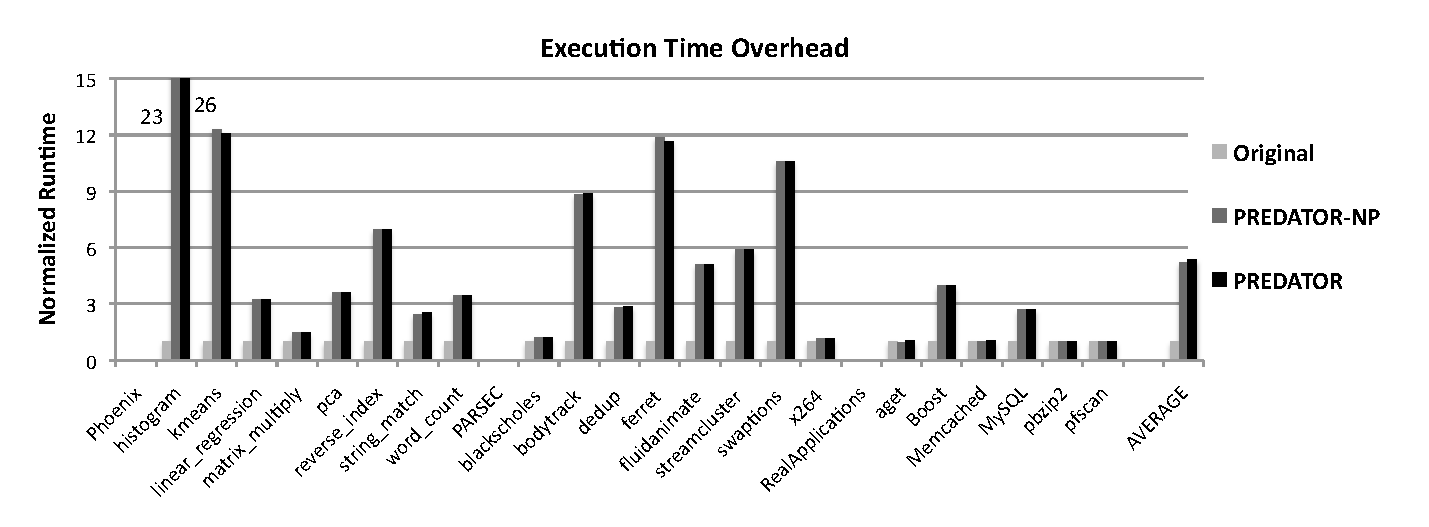
\includegraphics[width=6in]{predator/figure/perf}
\caption{
Performance overhead of \Predator{} with and without prediction(PREDATOR-NP).
\label{fig:perf}}
\end{figure*}
We perform evaluations on different benchmarks and application $10$ times and show the average of $8$ runs in in Figure~\ref{fig:perf}. To avoid the effect caused by extreme outliers, the maximum and minimum values are excluded here. 

For $16$ benchmarks from the Phoenix and PARSEC benchmark suites and six real applications, \Predator{} imposes $5.4\times$ performance overhead averagely. There is no noticeable difference on performance whether the prediction mechanism is enabled or not. 
 
Among five of these programs, histogram, kmeans, bodytrack, ferret, and swaptions, \predator{} introduces more than $8\times$ performance overhead. The histogram benchmark runs more than $26\times$ slower than the one with \pthreads{}, because tracking detailed access on cache lines with false sharing exacerbates the false sharing effect (see more discussion in Section~\ref{sec:sample}).  For bodytrack and ferret, although there is no false sharing, \Predator{} detects a large amount of cache lines with writes larger than {\it Tracking-Threshold}. Thus, tracking those accessing details for those cache lines imposes significant performance overhead. Currently, we have not identified the exact cause of \Predator{}'s high performance for kmeans.
   
\Predator{} imposes a small performance overhead for IO-bound applications, such as matrix\_multiply, blackscholes, x264, aget, Memcached, pbzip2, and pfscan, since \Predator{} does not add any performance overhead for IO operations.  

\subsection{Memory Overhead}
\label{sec:memoverhead}
We evaluate physical memory overhead of \Predator{}, instead of virtual memory overhead, because \Predator{} allocates 4GB virtual memory for its custom memory allocator beforehand. Proportional set size (PSS) of a specific memory mapping (in \texttt{/proc/self/smaps}) reflects the physical memory increase because of running the current application~\cite{memusage}. Thus, we periodically collect this data and use the sum of different memory mappings as the total physical memory usage of running an application. Figure~\ref{fig:memusage} presents the normalized physical memory usage of running different applications, comparing to that using \pthreads{}. 

\Predator{} imposes less than 50\% memory overhead for 17 out of 22 applications.  For swaptions and aget, \Predator{} introduces more memory overhead because the original memory footprints of them are very small, only $3$ kilobytes. Adding the code of detection, prediction and reporting (constant overhead) contributes to a large ratio of memory overhead. The increase of memory consumption in MySQL, from 132 MB to 512 MB, is due to \Predator{}'s heap organization, which does not aggressively reclaim memory held by individual threads. In all cases where \Predator{}'s imposes substantial memory overhead, the applications continue to comfortably fit into RAM on modern platforms.


\subsection{Sampling Rate Sensitivity}
\label{sec:predatorsensitivity}
Section~\ref{sec:sample} describes \Predator{}'s sampling mechanism to reduce tracking overhead. This section evaluates the effect of different sampling rates on performance and effectiveness. Note that running an application with different sampling rates does not affect its memory usage, thus memory overhead is not examined here. 

The default sampling rate used by \Predator{} is 1\%. In this section, we also evaluate two other sampling rates, 0.1\% and 10\%. Figure~\ref{fig:predatorsample} presents performance results under the three different sample rates. We only show the results of those programs having false sharing problems inside, since only their performance are most likely to be affected by different sampling rates. As expected, \Predator{} introduces less performance overhead under a lower sampling rate, but with a very minor performance impact. About effectiveness, even when using the 0.1\% sampling rate, \Predator{} can still detect all false sharing problems, although it reports a lower number of cache invalidations. Thus, different sampling rates do not affect the detection effectiveness.
 
\begin{figure*}[!t]
\centering
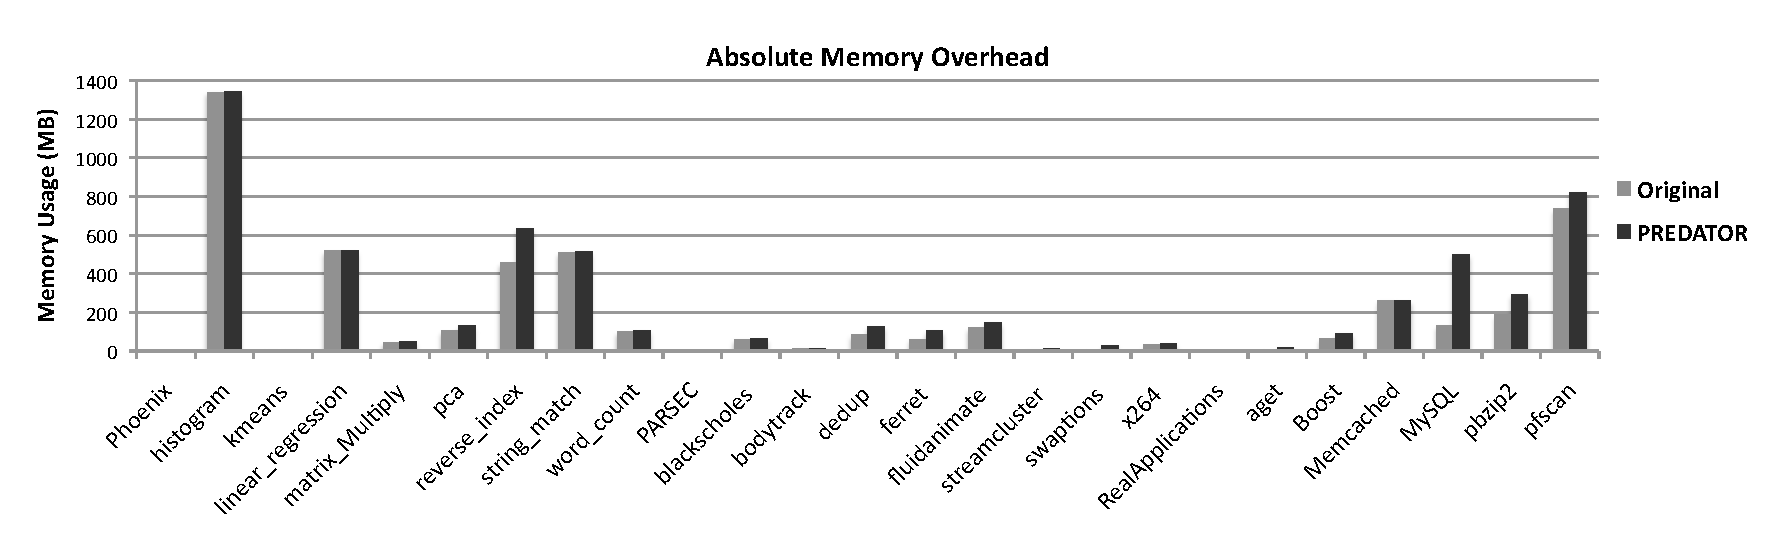
\includegraphics[width=6in]{predator/figure/absolutememory}
\caption{Absolute physical memory usage overhead with \Predator{}.}
\label{fig:absolutememusage}
\end{figure*}

\begin{figure*}[!t]
\centering
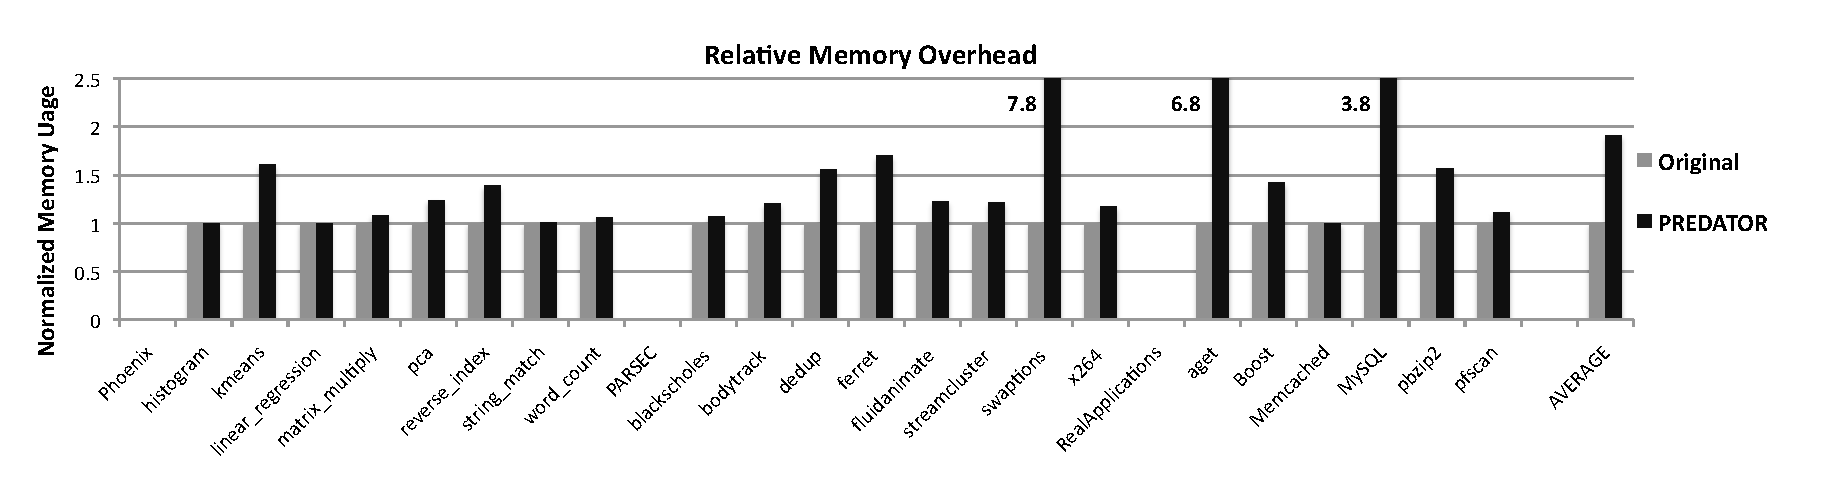
\includegraphics[width=6in]{predator/figure/memusage}
\caption{Relative physical memory usage overhead with \Predator{}.}
\label{fig:memusage}
\end{figure*}

\begin{figure}[!t]
\centering
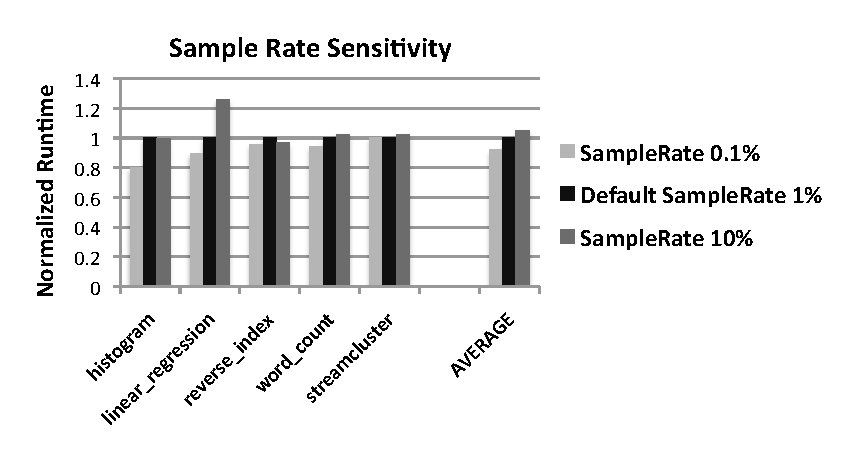
\includegraphics[width=6in]{predator/figure/sample}
%\includegraphics{fig/potential.pdf}
\caption{Sampling rate sensitivity (execution time).}
\label{fig:predatorsample}
\end{figure}




\section{Discussion}
\label{sec:discussion}

\subsection{Instrumentation Selection}
\label{sec:instrumentationtradeoff}
Dynamic binary instrumentation and compiler-based instrumentation are two alternative approaches to perform instrumentation~\cite{Instrumentation}. They exhibit different tradeoffs of performance and generality. Dynamic binary instrumentors, such as Valgrind~\cite{Valgrind}, Pin~\cite{Pin}, and DynamoRIO~\cite{DynamoRIO}, typically analyze the program's code just before execution in order to insert instrumentation. They introduce significant performance overhead, mostly caused by run-time encoding and decoding, but the fact that they operate directly on binaries makes them extremely convenient. By contrast, compiler instrumentation inserts instrumentation in the compilation phase, which requires re-compilation of all source code. 
\Predator{} employs compiler-based instrumentation both because of its better performance and its greater flexibility, as discussed in Section~\ref{sec:selectinstrumentation}.

\subsection{Effectiveness}
Several factors can affect \Predator{}'s ability to identify false sharing.

\emph{Different Inputs.} Different inputs trigger distinct executions of a program. If a specific input does not exercise the code with false sharing problems, \Predator{} cannot necessarily detect them. However, \Predator{} does generalize over inputs to find latent false sharing problems on those exercised code. When any reasonably representative set of inputs are exercised, as is required by any testing regime, \Predator{} can effectively predict false sharing.

\emph{Input Size.} Input size may affect detection results.  As discussed in Section~\ref{optimization}, \Predator{} introduces several threshold values to reduce tracking overhead, which can be adjusted as needed. If the input size is so small that it cannot generate enough false sharing events to cross the pre-defined thresholds, then the detection mechanism will not be triggered. In such cases, \Predator{} will miss actual cases of false sharing. However, realistically large inputs should be enough to trigger \Predator{}'s detection mechanisms. 

\emph{Hardware Independence.}  \Predator{}'s compiler-based approach make it independent of the underlying hardware platform. This approach increases generality, but may lead to over-report false sharing. \Predator{} conservatively assumes that different threads are running on different cores and detects false sharing problems based on possible cache invalidations. However, if multiple threads involved in false sharing are on the same core, then there will be no performance impact. 

%\subsection{Prediction Limitations} 
%\Predator{} can accurately and precisely predict a false sharing problem even when it does not occur. But \Predator{} cannot predict a false sharing problem if the code with false sharing is not exercised at all. Also, \Predator{} may miss potential false sharing problems between two objects brought by a different compiler or memory allocator. 




\chapter{Related Work}

\label{chapter:relatedwork}
This chapter first describes those related work to processes-as-threads framework and deterministic execution. Then it describes related work in false sharing detection, prevention, or both. 

\section{Processes-As-Threads framework}

BOP relies on strong isolation of processes to automatically and safely parallelize the execution of programs~\cite{DingBOP}. BOP forks a new process to do speculation, based on those pre-defined possibly parallel regions (PPR). In order to check the correctness, BOP tracks accesses on a page-based granularity. When there is no conflict and a speculative process reaches the end of its current PPR, its predecessor always commits its changes to the current process. However, BOP does not provide any synchronization support and cannot be used to run normal multithreaded programs. 

Grace is a process-based approach designed to prevent
concurrency errors, such as deadlock, race conditions, and
atomicity errors by imposing a sequential semantics on
speculatively-executed threads~\cite{grace}. Grace supports only fork-join programs without inter-thread communication (e.g., condition variables or barriers), and rolls back threads when accesses of threads would violate sequential semantics: a thread accesses pages that have been accessed by its predecessors. Grace cannot support arbitrary multithreaded programs. Similar to the Grace system, Sammati is a processes-as-threads system to detect and tolerate deadlock problems~\cite{Pyla:2010:ADA:1854273.1854288}. However, Sammati does not support the full range of synchronizations, without the support of conditional variables, barriers, and signals. Also, Semmati cannot avoid race conditions happening in creating twin pages, which are avoided by the \Sheriff{} framework.

\begin{comment}
% Some usage of this framework
According to Revisions,  Grace cannot easily resolve all
conflicts on commit (like revisions do) and must thus restrict
tasks from producing such conflicts either statically (by type
system) or dynamically (pessimistic with blocking, or optimistic with abort and retry). Also, Grace allows only a restricted “fork-join” form of concurrency
Revisions~\ref{Burckhardt:2010:CPR:1869459.1869515}
\end{comment}

\section{Deterministic Multithreading}
The research on deterministic multithreading is a very active area these years. We describe some software-only, non- language-based approaches here.

Grace prevents deadlocks, race conditions, ordering and atomicity violations errors for those fork-join multithreaded programs by imposing a sequential semantics at join points~\cite{grace}. However, Grace does not support programs with inter-thread communications, such as conditional variables and barriers.

CoreDet is a compiler-based approach to 
support general-purpose multithreaded programs~\cite{Bergan:2010:CCR:1736020.1736029}. 
CoreDet instruments those memory read and write operations as long
as those operations cannot be proved to be thread-local in static analysis. 
In the runtime phase, CoreDet divides the execution into 
alternating parallel and serial phases and guides all memory operations 
using a memory ownership table: only those owned locations can be accessed
in the parallel phases; all non-owned locations and synchronizations can only 
be accessed in the serial phases guided by a global token.
CoreDet guarantees deterministic execution for racy programs without memory errors,
but with very high performance overhead: 
averagely $3.5\times$ slower than those using \pthreads{}.
In order to guarantee determinism, 
CoreDet has to serialize \emph{all} external library calls without instrumentation.
CoreDet does not provide deterministic 
memory allocations, which can not guarantee determinism for programs with memory errors.  
% The use of synchronization points as commit boundaries also makes \dthreads{}
% code relatively \emph{robust}: when updates occur after a given number of 
% instructions retired (as in CoreDet and Kendo), it is impossible for 
% programmers to know when interleavings can occur. Such boundaries could vary 
% depending on the underlying architecture and would also be input-dependent, 
% meaning that slightly different inputs could lead to dramatically different
% thread interleavings. By contrast, \dthreads{} guarantees that only changes to
% the sequence of synchronization operations affect the order in which updates 
% are applied.
dOS~\cite{deterministic-process-groups} is an extension to CoreDet that uses the same deterministic scheduling framework.  dOS supports deterministic communication for those threads and processes inside the same
deterministic process groups (DPGs) and handle those external non-determinism by recording and
replaying interactions across DPG boundaries. 

Determinator is a microkernel-based operating system that enforces system-wide determinism~\cite{efficient-system-enforced}. Determinator provides separate address spaces and supports interprocess
communications at explicit synchronization points. 
Determinator is a proof-of-concept system, which can not support the whole rage of
threads APIs and can not work on legacy programs.  

Some other works can only support limited determinism or need user annotation.
Kendo can only guarantee the determinism for race-free programs~\cite{1508256}. 
TERN~\cite{stable-deterministic} provides a best-effort system to apply memoized schedules for future runs with similar inputs. 
It can not guarantee the determinism for racy programs, as Kendo. 
Peregrine~\cite{peregrine:sosp11} is a system based on TERN, which tries to record the order of memory accesses for racy portions and apply those schedules for future runs possibly.
However, both TERN and Peregrine do not support complete determinism (using a best effort) and requires program annotations. 

\section{False Sharing}

This section describes related work in false sharing detection, prevention, or both. There is no previous
system to predict unobserved false sharing.

\subsection{False Sharing Detection}
Based on the SIMICS functional simulator, Schindewolf et al.\ designed a tool to report different kinds of cache usage information, such as cache misses and cache invalidations~\cite{falseshare:simulator}. Pluto relies on Valgrind dynamic instrumentation framework to track the sequence of memory read and write events on different threads, and reports a worst-case estimation of possible false sharing~\cite{falseshare:binaryinstrumentation1}.
Similarly, Liu uses Pin to collect memory access information, and reports total cache miss information~\cite{falseshare:binaryinstrumentation2}.
These tools impose about $100-200\times$ performance overhead.

Zhao et al.\ developed a tool based on DynamoRIO framework to detect false sharing and other cache contention problems
for multithreaded programs~\cite{qinzhao}. 
It uses a shadow memory technique to maintain memory access history and detects cache invalidations based on the ownership of cache lines. However, it can only support at most $8$ threads currently and it is hard to scale up, because of its per-bit-each-thread bitmap design. In addition, it cannot differentiate cold cache misses from actual false sharing problems.

Intel's performance tuning utility (PTU) uses Precise Event Based Sampling (PEBS) hardware support to detect false sharing problems ~\cite{detect:ptu, detect:intel}.  PTU cannot distinguish true sharing from false sharing. In addition, PTU aggregates memory accesses without considering memory reuses and access interleaving, leading to numerous false positives. Sanath et al. designed a machine learning based approach to detect false sharing problems. They train their classifier on mini-programs and apply this classifier to general programs ~\cite{mldetect}. Instead of instrumenting memory accesses, this tool relies on hardware performance counters to collect memory accesses events. It achieves very low performance overhead (about 2\%). But it relies on hardware support for its efficiency.  Also, it cannot detect a lot of actual false sharing problems that can greatly affect performance, such as histogram and streamcluster. We guess that this incompleteness can be caused by their problematic training method or hardware's sampling mechanism, but the specific reason is not clear to us. 

In addition to their individual disadvantages,
all approaches discussed above share two common shortcomings:  
They cannot pinpoint the exact location of false sharing in the source code, so programmers have to examine the source code and identify problems manually; they can only detect those observed false sharing problems. 

Pesterev et al.\ present DProf, a tool that help programmers identify cache misses based on AMD's instruction-based sampling hardware~\cite{DProf}. DProf requires manual annotation to locate data types and object fields, and cannot detect false sharing when multiple objects reside on the same cache line.

\subsection{False Sharing Prevention}
\label{sec:fspreventwork}
% More approaches
Jeremiassen and Eggers use a compiler transformation to automatically adjust the memory layout of applications through padding and alignment~\cite{falseshare:compile}. Chow et al.\ alter parallel loop scheduling in order to avoid false
sharing~\cite{falseshare:schedule}. These approaches only works for regular, array-based scientific code.

Berger et al.\ describe Hoard, a scalable memory allocator that can reduce the possibility of false sharing by making different threads use different heaps~\cite{Hoard}. Hoard cannot avoid false sharing problem in global variables or within
a single heap object: the latter appears to be the primary source of real false sharing problems.

\subsection{False Sharing Detection and Prevention}

Plastic leverages the sub-page granularity memory remapping facility provided by the Xen hypervisor to detect and tolerate false sharing automatically~\cite{OSdetection}. However, the sub-page memory remapping mechanism is not currently supported by most existing operating system, reducing its generality. In addition, Plastic cannot pinpoint the exact source of false sharing.  
In order to utilize Plastic's prevention tool, a program has to run on the Xen hypervisor, limiting the applicability of their prevention technique.



\chapter{Conclusions and Future Work}
\label{chapter:conclusion}

Because of hard physical limits, computer manufacturers have turned to providing more and more cores on a single machine. This phenomenon drives the biggest revolution of software development: software has to be programmed in a concurrent and parallel way in order to exploit the benefits of multi-core machines.

Building efficient and reliable concurrent software is still a challenging task. First, concurrency requires programmers to think in an unnatural way that humans find difficult.  Second, existing languages and tools are inadequate to detect or prevent concurrency errors.  

\section{Contributions}

This thesis helps boost the performance and ease the reasoning and debugging, by providing different tools and runtime systems. We present a novel processes-as-threads replacement library, the \sheriff{} framework, which providing per-thread memory protection and isolation on the page granularity. First, based on this framework, we provide \dthreads{} to ensure deterministic execution of multithreaded programs, even with race conditions. \dthreads{} outperforms the previous state-of-the-art runtime system (CoreDet) by a factor of 3, and is the new basis of all later deterministic multithreading systems. Second, we presents two tools based on the \Sheriff{} framework, \SheriffDetect{} and \SheriffProtect{}, to deal with false sharing problems of multithreaded programs, one of the notorious performance problems. \SheriffDetect{} is the first tool to correctly and precisely identify false sharing problems inside parallel applications. \SheriffProtect{} is the first generalized system to automatically mitigate false sharing problems, without the need of programmer intervention.  Finally, we present another tool, \predator{}, to improve the effectiveness by revealing read-write false sharing problems and overcome a generalized issue of false sharing detection: Existing tools can only detect those observed false sharing problems; \Predator{} can predict potential false sharing that does not manifest in a given execution but may appear---and greatly degrade application performance—--in a slightly different execution environment. \Predator{} is the first false sharing tool that is able to automatically and precisely uncover false sharing problems in real applications, including MySQL and the Boost library.

\section{Future Work}

\dthreads{} performs synchronizations inside serial phases, which is susceptible to delays due to load imbalance between threads. To handle this problem, one direction of future work is to reduce the waiting time caused by load imbalance problem. We observed that the overhead of \dthreads{} depends on the number of synchronizations: with less synchronizations, \dthreads{} can achieve much better performance since it can amortize the overhead better.  Another direction of future work is to design programs with \dthreads{}'s mechanism in mind, by extending a set of APIs, so that users can design programs with less load imbalance problem and less synchronizations. Thus, we could possibly achieve better performance. 

This thesis also presents a set of tools to detect false sharing problems inside multithreaded programs. But false sharing problems can exist in the entire software stack, including hypervisors, operating systems, and applications using different threading libraries or other languages. In the future, we would like to extend the detection mechanism, coming from \predator{}, to the entire software stack. Also, we can leverage memory trace information to suggest fixes, in order to help programmers to eliminate false sharing.

\SheriffProtect{} introduces some performance overhead when a parallel program does not have false sharing problem inside. It is helpful if this protection mechanism can leverage the output of detection: we only use this mechanism to boost the performance if an application has some false sharing problems inside; further, we can employ isolation on specific objects in order to further reduce performance overhead.  

%%
%% Beginning of back matter
\backmatter  %% <--- mandatory

%%
%% We don't support endnotes

%%
%% A bibliography is required.
\bibliographystyle{umthesis}
\bibliography{refs}
\end{document}

%%% Local Variables: 
%%% mode: latex
%%% TeX-master: t
%%% End: 
